% !TeX encoding = UTF-8
% !TeX program = xelatex
% !TeX spellcheck = en_US

\documentclass[degree=master]{thuthesis}
  % 学位 degree:
  %   doctor | master | bachelor | postdoc
  % 学位类型 degree-type:
  %   academic(默认)| professional
  % 语言 language
  %   chinese(默认)| english
  % 字体库 fontset
  %   windows | mac | fandol | ubuntu
  % 建议终版使用 Windows 平台的字体编译


% 论文基本配置,加载宏包等全局配置
% !TeX root = ./thuthesis-example.tex

% 论文基本信息配置

\thusetup{
  %******************************
  % 注意:
  %   1. 配置里面不要出现空行
  %   2. 不需要的配置信息可以删除
  %   3. 建议先阅读文档中所有关于选项的说明
  %******************************
  %
  % 输出格式
  %   选择打印版(print)或用于提交的电子版(electronic),前者会插入空白页以便直接双面打印
  %
  output = print,
  %
  % 标题
  %   可使用“\\”命令手动控制换行
  %
  title  = {多源时间序列对称模式挖掘研究},
  title* = {Research on Symmetric Pattern Mining of Multi-source Time Series},
  %
  % 学位
  %   1. 学术型
  %      - 中文
  %        需注明所属的学科门类,例如:
  %        哲学、经济学、法学、教育学、文学、历史学、理学、工学、农学、医学、
  %        军事学、管理学、艺术学
  %      - 英文
  %        博士:Doctor of Philosophy
  %        硕士:
  %          哲学、文学、历史学、法学、教育学、艺术学门类,公共管理学科
  %          填写“Master of Arts“,其它填写“Master of Science”
  %   2. 专业型
  %      直接填写专业学位的名称,例如:
  %      教育博士、工程硕士等
  %      Doctor of Education, Master of Engineering
  %   3. 本科生不需要填写
  %
  degree-name  = {工程硕士},
  degree-name* = {Master of Engineering},
  %
  % 培养单位
  %   填写所属院系的全名
  %
  department = {软件学院},
  %
  % 学科
  %   1. 学术型学位
  %      获得一级学科授权的学科填写一级学科名称,其他填写二级学科名称
  %   2. 工程硕士
  %      工程领域名称
  %   3. 其他专业型学位
  %      不填写此项
  %   4. 本科生填写专业名称,第二学位论文需标注“(第二学位)”
  %
  discipline  = {软件工程},
  discipline* = {Software Engineering},
  %
  % 姓名
  %
  author  = {李盼盼},
  author* = {Li Panpan},
  %
  % 指导教师
  %   中文姓名和职称之间以英文逗号“,”分开,下同
  %
  supervisor  = {宋韶旭, 副教授},
  supervisor* = {Associate Professor Song Shaoxu},
  %
  % 副指导教师
  %
  % associate-supervisor  = {陈文光, 教授},
  % associate-supervisor* = {Professor Chen Wenguang},
  %
  % 联合指导教师
  %
  % co-supervisor  = {某某某, 教授},
  % co-supervisor* = {Professor Mou Moumou},
  %
  % 日期
  %   使用 ISO 格式;默认为当前时间
  %
  % date = {2019-07-07},
  %
  % 是否在中文封面后的空白页生成书脊(默认 false)
  %
  include-spine = false,
  %
  % 密级和年限
  %   秘密, 机密, 绝密
  %
  % secret-level = {秘密},
  % secret-year  = {10},
  %
  % 博士后专有部分
  %
  % clc                = {分类号},
  % udc                = {UDC},
  % id                 = {编号},
  % discipline-level-1 = {计算机科学与技术},  % 流动站(一级学科)名称
  % discipline-level-2 = {系统结构},          % 专业(二级学科)名称
  % start-date         = {2011-07-01},        % 研究工作起始时间
}

% 载入所需的宏包

% 定理类环境宏包
\usepackage{amsthm}
% 也可以使用 ntheorem
% \usepackage[amsmath,thmmarks,hyperref]{ntheorem}

\thusetup{
  %
  % 数学字体
  % math-style = GB,  % GB | ISO | TeX
  math-font  = xits,  % sitx | xits | libertinus
}

% 可以使用 nomencl 生成符号和缩略语说明
% \usepackage{nomencl}
% \makenomenclature

% 表格加脚注
\usepackage{threeparttable}

% 表格中支持跨行
\usepackage{multirow}

% 固定宽度的表格。
% \usepackage{tabularx}

% 跨页表格
\usepackage{longtable}

% 算法
\usepackage{algorithm}
\usepackage{algorithmic}

% 量和单位
\usepackage{siunitx}

% 参考文献使用 BibTeX + natbib 宏包
% 顺序编码制
\usepackage[sort]{natbib}
\bibliographystyle{thuthesis-numeric}

% 著者-出版年制
% \usepackage{natbib}
% \bibliographystyle{thuthesis-author-year}

% 本科生参考文献的著录格式
% \usepackage[sort]{natbib}
% \bibliographystyle{thuthesis-bachelor}

% 参考文献使用 BibLaTeX 宏包
% \usepackage[style=thuthesis-numeric]{biblatex}
% \usepackage[style=thuthesis-author-year]{biblatex}
% \usepackage[style=apa]{biblatex}
% \usepackage[style=mla-new]{biblatex}
% 声明 BibLaTeX 的数据库
% \addbibresource{ref/refs.bib}

% 定义所有的图片文件在 figures 子目录下
\graphicspath{{figures/}}

% 数学命令
\makeatletter
\newcommand\dif{%  % 微分符号
  \mathop{}\!%
  \ifthu@math@style@TeX
    d%
  \else
    \mathrm{d}%
  \fi
}
\makeatother

% hyperref 宏包在最后调用
\usepackage{hyperref}



\begin{document}

% 封面
\maketitle

% 学位论文指导小组、公开评阅人和答辩委员会名单
% 本科生不需要
\input{data/committee}

% 使用授权的说明
\copyrightpage
% 将签字扫描后授权文件 scan-copyright.pdf 替换原始页面
% \copyrightpage[file=scan-copyright.pdf]

\frontmatter
% !TeX root = ../thuthesis-example.tex

% 中英文摘要和关键字

\begin{abstract}
  信息技术和工业经济的融合催生出了智能化和数字化的现代工业,
  同时也产生了规模庞大的工业数据。
  时间序列是一种典型的工业大数据,蕴含着丰富的
  规律和知识。其中,对称子段作为一种
  具有前后对应特征的时序子段,广泛分布于多种时间序列之中。
  挖掘对称子段在轨迹分析、异常识别和序列预测等领域具有重要的
  研究价值。然而,工业时间序列的随机误差和超大数据量给
  对称子段的挖掘带来了困难。基于此,
  本文研究了一类时间和空间效率均较为高效的
  对称子段挖掘算法来应对上述问题。

  % 再度量子序列的对称性
  % 对称模式涉及到时间序列的对比与匹配。
  % 因此,时间序列的相似性度量对
  % 对称模式挖掘算法的效果和性能具有决定性作用。
  % 一种简单的序列相似性度量算法是欧式距离。
  % 但是欧氏距离采用一一对应的点匹配策略,
  % 对时间序列偏移、缺失和形状变化等比较敏感。
  % 动态时间扭曲(DTW)通过弯曲时间序列使得每个点有多个匹配候选,
  % 从而提高了相似性度量算法的鲁棒性。
  % 但工业应用中时间序列的数据量往往高达几十甚至上百GB,
  % 动态时间扭曲算法的计算效率堪忧。

  对称子段判定算法是解决对称子段挖掘问题的基础。
  对于对称子段判定问题,准确的对称性度量算法是其关节所在。
  欧氏距离度量是一种简单而有效的算法,
  但其一一对应的点匹配策略,对时间序列
  偏移、缺失和形状变化比较敏感。
  本文提出了一个基于最优匹配和自适应阈值的
  对称子段判定算法,对时间序列各类异常具有很好的鲁棒性。
  经过实验证明,本算法在
  对称子段判定效果上超过了
  利用欧氏距离和动态时间扭曲度量对称性的算法。并且,
  本文还通过优化对称度计算方式将对称子段判定算法扩展到了
  流式时间序列,在保证时间性能的同时,将算法的空间复杂度
  优化至了$O(n)$,为对称子段判定在大数据上的应用提供了可能。

  对称子段挖掘除了要对子段对称性进行判定,
  还需要对时间序列进行分段处理并解决子段重叠问题。
  因此,根据区间动态规划算法思想,
  结合滑动窗口模型和贪心策略,本文设计了一种渐进时间复杂度为
  $O\left( \left| X \right| \times w \right)$的
  对称子段挖掘算法。
  经过实验证明,
  本文提出的算法不但保持了对称子段挖掘效果的准确性,
  而且相比基于动态时间扭曲的算法在效率上
  有了100倍以上的提升。
  此外,根据IoTDB的存储和计算方式,本文设计了基于
  UDF和元数据的两种算法实现,分别适用于写入和查询负载较重
  的应用场景,在系统层面对对称子段挖掘算法进行了扩展。

  通过对对称子段判定和挖掘算法的研究与实验,我们发现,
  本文提出的算法不仅在挖掘效果上具有很好的准确性和鲁棒性,
  在性能上也高于基于动态时间扭曲的算法,
  而且在复杂应用场景有很好的可扩展性。
  最后,本文在IoTDB系统上实现了对称子段判定和挖掘算法,
  完善了IoTDB挖掘时间序列特定类型子段的功能,
  为用户数据分析提供有价值的信息。
  
  % 关键词用“英文逗号”分隔,输出时会自动处理为正确的分隔符
  \thusetup{
    keywords = {时间序列, 相似性度量, 对称子段, 动态规划},
  }
\end{abstract}

\begin{abstract*}
  The integration of information technology and 
  industrial economy has given birth to intelligent 
  and digital modern industries, as well as 
  large-scale industrial data. Time series is a 
  typical industrial big data, which contains rich 
  laws and knowledge. Among them, the symmetric 
  subsegment, as a type of time series subsegment 
  with corresponding features before and after, 
  is widely distributed in various time series. 
  Mining symmetric subsegments has important research 
  value in the fields of trajectory analysis, 
  anomaly identification and sequence prediction. 
  However, the random errors and large data volume of 
  industrial time series bring difficulties to the mining 
  of symmetric subsegments. Based on this, this paper 
  studies a type of symmetric subsegment mining 
  methods that are both efficient in time and space 
  to deal with the above problems.

  Symmetric subsegment judgment algorithm is the 
  basis to solve the problem of symmetric subsegment 
  mining. For the symmetric subsegment judgment problem, 
  the accurate symmetry measurement algorithm is 
  where its joints are located. Euclidean distance 
  metric is a simple and effective method, but its 
  one-to-one correspondence point matching strategy 
  is sensitive to time series offset, missing and 
  shape changes. In this paper, a symmetric subsegment 
  judgment algorithm based on optimal matching and 
  adaptive threshold is proposed, which has good 
  robustness to various anomalies in time series. 
  Experiments show that this method surpasses the 
  method of using Euclidean distance and dynamic 
  time warping to measure symmetry in judging the 
  effect of symmetric subsegemnts. In addition, 
  this paper also extends the symmetric subsegment 
  judgment algorithm to streaming time series 
  by optimizing the calculation method of symmetry 
  degree. While ensuring the time performance, 
  the space complexity of the algorithm is optimized 
  to $O(n)$, for the symmetric subsegment judgment 
  in the application of big data provides the 
  possibility.

  In addition to judging the symmetry of subsegments, 
  symmetric subsegment mining also needs to segment 
  the time series and solve the problem of overlapping 
  subsegments. Therefore, according to the idea of 
  interval dynamic programming algorithm, combined 
  with sliding window model and greedy strategy, 
  this paper designs a symmetric subsegment mining 
  algorithm with asymptotic time complexity 
  $O\left( \left| X \right| \times w \right)$. 
  Experiments show that the mining algorithm proposed 
  in this paper not only maintains the accuracy of 
  the subsegment mining methods, but also improves 
  the efficiency by more than 100 times compared 
  with the algorithm based on dynamic time warping. 
  In addition, according to the storage and computing 
  methods of IoTDB, this paper implements two mining 
  algorithms based on UDF and metadata, which are 
  suitable for application scenarios with heavy write 
  and query loads respectively, and the symmetric 
  subsegment mining algorithm is extended at the 
  system level.

  Through the research and experiments on the 
  symmetric subsegment judgment and mining algorithm, 
  we found that the method proposed in this paper 
  not only has good accuracy and robustness in 
  mining effect, but also has higher performance 
  than the algorithm based on dynamic time warping. 
  And it has good scalability in complex application 
  scenarios. Finally, this paper implements the 
  symmetric subsegment judgment and mining algorithm 
  on the IoTDB system, improves the function of IoTDB 
  to mine specific time series subsegments, and 
  provides valuable information for user data analysis.

  % Use comma as separator when inputting
  \thusetup{
    keywords* = {time series, symmetric subsegment, similarity measure, dynamic programming},
  }
\end{abstract*}


% 目录
\tableofcontents

% 插图和附表清单
% 本科生的插图索引和表格索引需要移至正文之后、参考文献前
% \listoffiguresandtables  % 插图和附表清单(仅限研究生)
\listoffigures           % 插图清单
\listoftables            % 附表清单

% 符号对照表
% \input{data/denotation}


% 正文部分
\mainmatter
% !TeX root = ../thuthesis-example.tex

\chapter{引言}

\section{研究背景与意义}
互联网、物联网、云计算等计算机科学技术经过长时间的共同发展与不断融合,
积累了规模庞大、种类繁多的海量数据,涉及计算机科学、宏观经济、
军事科技、医疗卫生等诸多领域。根据统计,谷歌每天处理分析超过数百
PB的数据,脸书每个月产生超过10PB的日志数据,百度每天处理将近100PB
的数据,而淘宝每天可以产生数十个TB的数据。截至2012年,
技术上可在合理时间内分析处理的数据集大小单位为艾字节(EB)。
在这些海量数据之中,有一类按照数据生成的时间顺序,把同一个变量或
记录的数据值,或者高维数据的一个元组,排列而成的记录数据信息,
被称为时间序列。时间序列是工业界应用广泛的、与时间维度相关的
高维数据,也是数据挖掘技术的一种主要研究对象。

大部分时间序列数据中数据点会随着时间的变化而产生一定的变化规律,
其中某些规律在同一个时间序列中多次重复出现,这类规律称为模式。
时间序列中蕴含着多种多样的模式,挖掘出时间序列中蕴含的模式,
既可以为未来的决策提供理论与数据支持,又可以检测、判断、预防突发
错误的出现,指导实际生产。因此,时间序列模式挖掘是时间序列分析和
数据挖掘中的重要组成部分。在多样化的模式中,对称模式因为具有独特的
物理意义,在多种应用场景的时间序列数据中大量出现,具有重要的
研究价值。然而,由于时间序列数据的特殊性,对称模式的挖掘也
存在许多困难。

时间序列对称模式包括两种类别,一种是具有全局对称性的时间序列,
另一种是某些具有对称性的时间子序列集合。对于全局对称时间序列来说,
从数学角度判断其对称性的方式十分简单,确定对称中心,
并计算中心一侧序列是否为另一侧的镜像即可。图~\ref{fig:symmetric_string}
展示了对称字符串序列示意图,该序列在“D”两侧的子串互为镜像,
则为对称(回文)字符串序列。然而,时间序列的对称性并不像回文字符串序列
的对称性具有非常严格的数学定义,并不存在严格统一的对称中心。
图~\ref{fig:no_symmetic_center}展示了血压测量中力感测电阻器(FSR)
信号的变化示意图,尽管在物理意义上一次心跳过程的压缩和舒张阶段时间序列
具有对称性。然而,由于压缩阶段和舒张阶段的时长不一致,
采集点的个数不同,其对称中心并不严格位于时间的中点。
因此,在计算序列对称性时,不能简单地查找对称中心并根据对称中心将时间序列
分段,以免计算的对称度不准确。除此之外,由于物理设备、数据采集和数据传输
中遇到的问题,实际应用场景中的时间序列可能不是等间隔采样的,导致不同阶段
的数据点密度不一致,这种情况同样会造成对称中心点的不确定性。
\begin{figure}
  \centering
  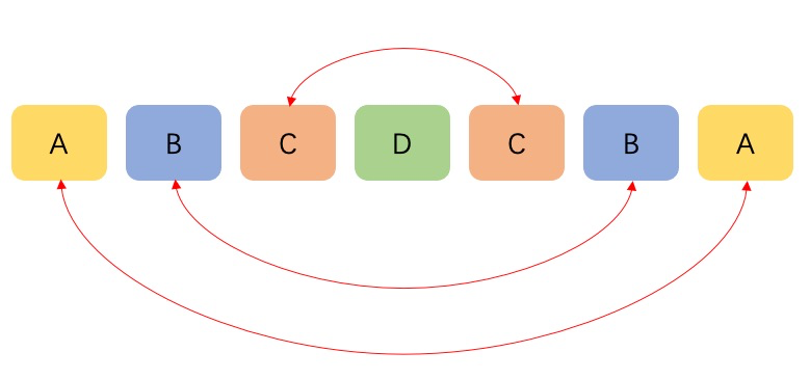
\includegraphics[width=0.86\linewidth]{symmetric_string.png}
  \caption{对称字符串序列}
  \label{fig:symmetric_string}
\end{figure}

\begin{figure}
  \centering
  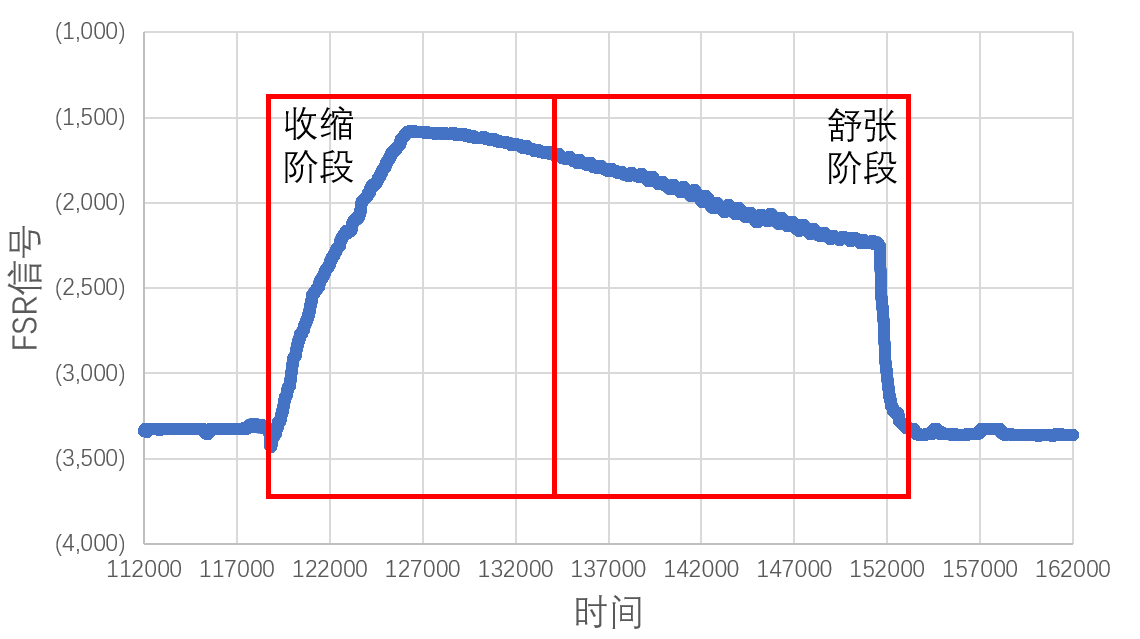
\includegraphics[width=0.86\linewidth]{no_symmetic_center.png}
  \caption{对称时间序列反映无严格对称中心的案例}
  \label{fig:no_symmetic_center}
\end{figure}

此外,由于采样频率不同以及数据随机性较大,时间序列在对称性匹配过程中
不可避免的存在一些失配现象。图~\ref{fig:mismatch}展示了某辆挖掘机
在作业过程中动臂提升工况的变化示意图,该序列为一次挖掘作业的动臂提升工况
时间序列,具有物理上的对称性。然而,由于抬臂阶段产生了红框所示的数据采集
缺失,导致动臂提升工况时间序列的抬臂和降臂阶段并不完全匹配。因此,
在对称模式的挖掘过程中,需要考虑到因为部分失配导致的对称度计算结果偏差问题。

除了利用对称中点截断时间序列计算对称性之外,使用原始时间序列和
其反转时间序列的相似性来度量对称性也是一种常见的方法。然而,
时间序列的对称性与时间间隔、序列模式和数据特征密切相关。在实际工业场景中,
原始和反转时间序列在时间线上不对齐的情况时有发生,不存在严格的一一对应关系,
使用传统的匹配方法,无法进行全局匹配度量。图1.4对比了某辆运煤车在行驶过程
中生成的纬度时间序列不同的匹配方式,可以看出,一一对应的匹配方式存在大量
的未对齐点,由此计算得到的对称度明显偏大。而全局匹配方式则应该从全局匹配
角度为原始和反转时间序列上的每对点求得最佳匹配,从而使计算得到的对称度最高。
因此,需要立足于时间序列的时间和全局数据特征挖掘时间序列的对称性。
\begin{figure}
  \centering
  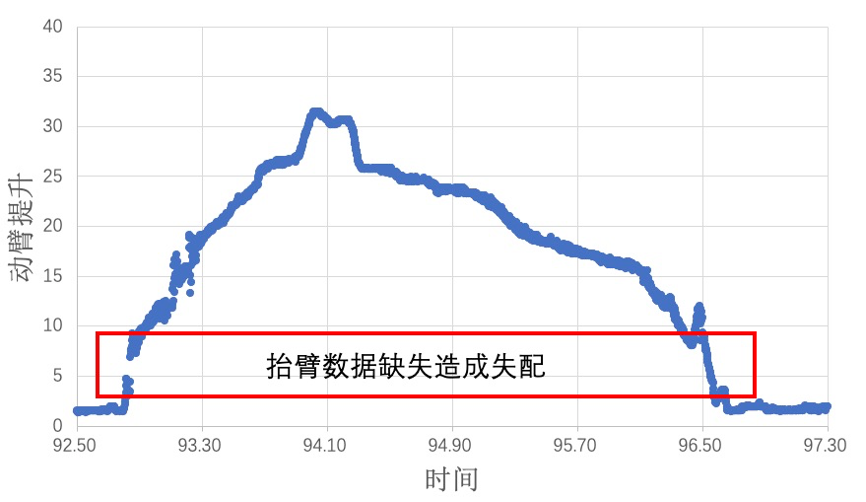
\includegraphics[width=0.86\linewidth]{mismatch.png}
  \caption{对称时间序列反映随机失配现象的案例}
  \label{fig:mismatch}
\end{figure}
\begin{figure}
  \centering
  \subcaptionbox{一一对应\label{fig:time_series_align-a}}
    {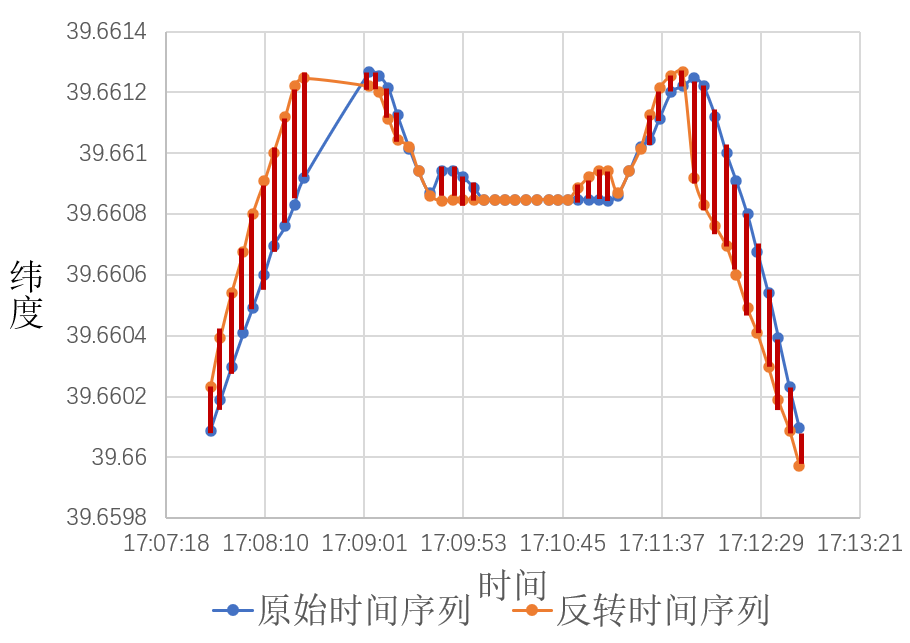
\includegraphics[width=0.43\linewidth]{time_series_align-a.png}}
  \subcaptionbox{全局匹配\label{fig:time_series_align-b}}
    {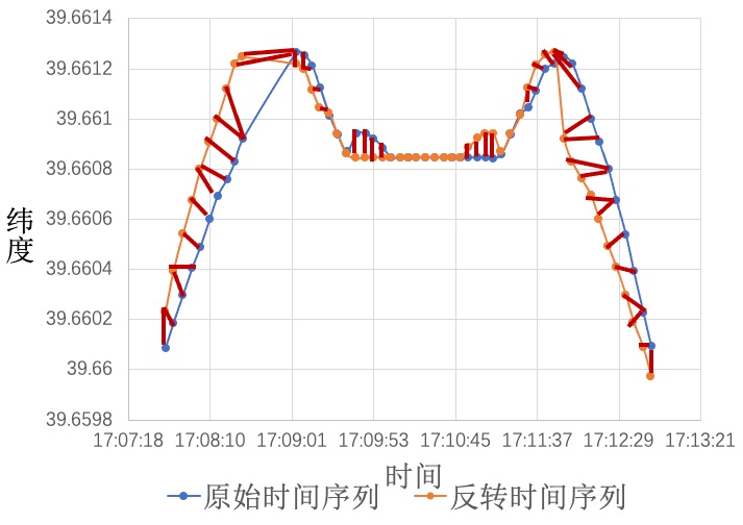
\includegraphics[width=0.43\linewidth]{time_series_align-b.png}}
  \caption{对称时间序列反映不对齐现象的案例}
  \label{fig:time_series_align}
\end{figure}

全局时间序列对称模式的挖掘需要立足于时间序列的整体数据特征。
然而,时间序列中可能蕴含着具有对称性的子模式。
图~\ref{fig:segement_symmetric_pattern}展示了在挖掘机
作业过程中斗臂外摆工况变化形成的时间序列。在该案例中,
多种对称子模式聚合在一条长时间序列之中,
由于传感器采样和数据传输的问题,存在包括
缺失点、异常点、噪声点等诸多问题,
这些问题都会干扰对称模式挖掘算法的效果。
并且,挖掘对称子模式需要设定子模式的长度以对长时间序列进行分段,
在给定时间序列的长度约束的前提下,挖掘出的对称子序列可能存在重叠情况,
从而导致后续数据分析和统计存在误差。
\begin{figure}
  \centering
  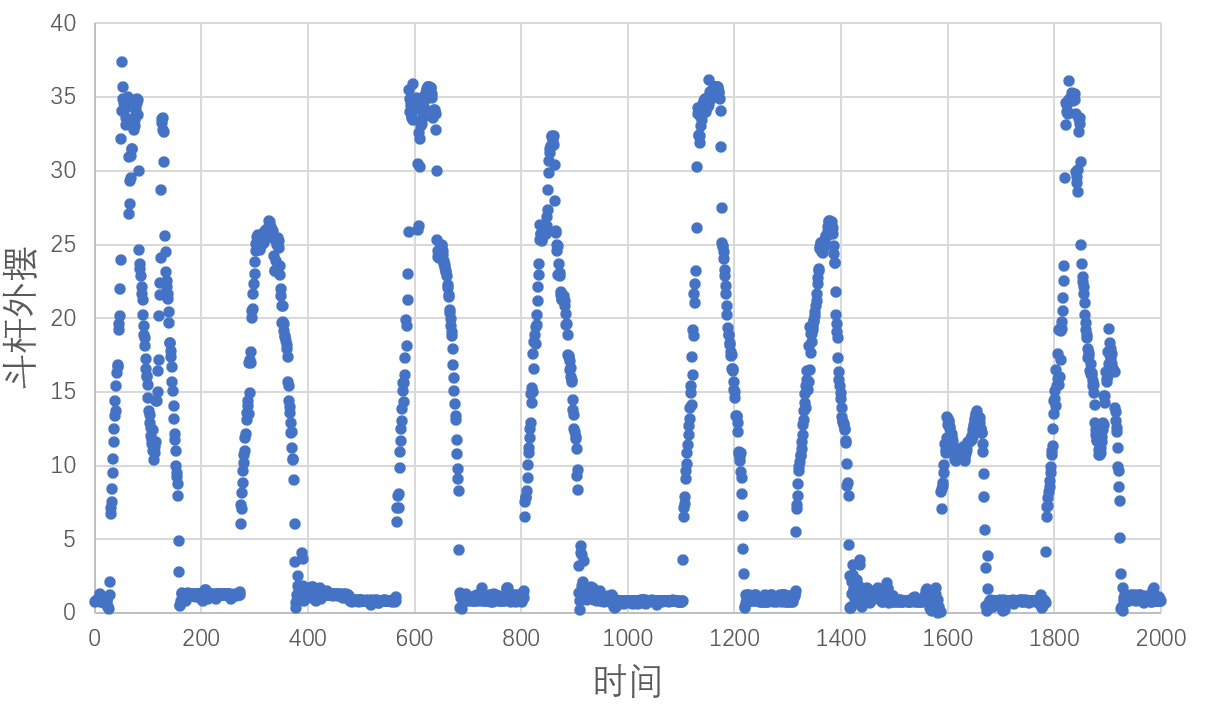
\includegraphics[width=0.86\linewidth]{global_symmetry.png}
  \caption{分段挖掘时间序列对称子模式的案例}
  \label{fig:segement_symmetric_pattern}
\end{figure}

总之,时间序列中的对称模式往往具有某种具体的物理意义,在血压监测图,
温度变化图和行车路线图等多种应用场景的时间序列数据中大量出现,挖掘
对称模式对于轨迹跟踪,作业分析,异常检测和序列预测都具有重要价值。
然而,时间序列的复杂性和不确定性为对称模式挖掘带来了诸多挑战。基于此,
本文提出了一类准确高效的时间序列对称模式挖掘方法,并将该方法扩展到了
流式数据和变长模式场景,通过实验验证了本方法的应用价值。


\section{研究内容与贡献}
为解决上述问题,本文将研究一类精确高效的时间序列对称模式挖掘方法,具体包含
以下三个方面:
\begin{enumerate}
  \item 全局时间序列的对称性并没有标准的度量方法,现有的基于对称中心与
  原始和反转时间序列的方法都存在问题。不同于回文字符串,时间序列并
  不存在严格统一的对称中心,通过对称中心截取子序列度量对称性的方法
  其效果极不稳定。直接通过原始时间序列和其反转时间序列的相似性度量
  对称性的方法可以避免确定对称中心的问题,但是重复计算,时间不对齐等
  问题也会导致对称性度量结果偏大,从而影响对称模式挖掘结果的准确性。
  因此,如何定义一种准确高效的时间序列对称性度量方法成了首要的目标。
  \item 在分段时间序列上挖掘对称子模式是一个多步骤的算法框架,
  不仅需要度量子序列的对称性,而且,对称时间子序列并不要求原始时间序列
  和其反转时间序列完全相同,只需要两者的距离在指定阈值范围内即可。
  因此,本文需要通过计算阈值来挖掘出真正的对称子序列。此外,时间序列中
  蕴含的对称模式可能存在重叠,需要设计算法过滤重叠的对称子序列,
  从而挖掘出不重叠的对称子序列集合,即对称模式。
  \item 对于流式数据上的对称模式挖掘,由于无法提前预知时间序列的全貌,
  静态的时间序列对称性度量算法失效。本文将研究如何使方法满足流式或
  分布式计算场景要求。流式计算场景要求方法只对数据进行一轮遍历且
  可增量执行。此外,时间序列中很可能存在长度不同的对称模式,
  为保证挖掘的完整性,需要研究可以自适应调整时间窗口大小的算法。
\end{enumerate}

基于以上的研究内容,本文主要贡献如下:
\begin{enumerate}
\item 定义了对称模式和全局时间序列对称性度量算法。
本文所挖掘的对称模式是关于中心点前后对称的时间序列模式,
其对称性由自定义的全局对称性度量算法进行计算,再根据时间序列
相邻点的距离特征作为阈值过滤对称时间序列做为对称模式。对称模式
在实际工业生产中非常常见,具有很高的应用价值。
\item 提出了分段时间序列对称模式的挖掘方法,并给出了具体的算法。
设定对称子序列的长度约束,采用分段对称性度量算法计算出时间子序列的对称度,
然后使用由时间序列数据特征和对称度分布特征确定的对称度阈值
分类得到对称子序列,最后根据获取数量最多对称子序列的贪心策略,
计算得到所有不重叠的对称模式。
\item 扩展了时间序列对称模式挖掘算法的应用,提高了算法的效率和模式挖掘的完整性。
针对流式数据实时到达的特征优化了对称模式挖掘的状态方程,
每生成一个新的数据点,实时计算出以当前数据点为终点的
子序列对称性,根据对称性阈值及时筛选出对称模式。
通过研究时间子序列对称性和窗口大小的关系,
分析建模了对称序列数据点差分的数据范围,
并根据范围自适应调整窗口大小,提高了对称模式挖掘的完整性。
\item 本文采用了来自UCR和真实工业场景中的时间序列数据集在
挖掘对称模式的F值,准确率、完整性以及时间开销方面进行了实验,
并与多种现有相关方法进行了对比。
结果表明:本文所提出的时间序列对称模式挖掘算法在
挖掘效果方面表现最优,同时在时间开销方面有着几乎最佳的性能。
此外,本文对对称模式挖掘算法进行了系统实现,把它们集成到
IoTDB数据质量分析工具IoTDB-Quality中。一方面,完善了
IoTDB-Quality工具的功能,弥补了工具在时间序列模式挖掘
上的功能缺失。另一方面,通过挖掘出时间序列中的对称模式,
工具可以继续对时间序列进行数据分析和异常检测,进一步推动了
IoTDB-Quality工具的应用。
\end{enumerate}

\section{论文组织结构}

本文共划分为 7 个章节,各个章节的组织内容如下所述:

第 1 章为引言部分,主要介绍了时间序列数据的特点和
对称模式挖掘的挑战,并据此引出本文的研究内容,
最后总结了本文的工作内容和贡献。

第 2 章介绍并定义了本文涉及到的概念知识,
即时间序列和对称模式。
之后对国内外在序列相似性度量和模式挖掘上的研究进行了
分类和阐述。

第 3 章提出时间序列对称模式挖掘方法,包括
全局对称模式和分段对称模式。
全局对称模式挖掘算法利用区间动态规划和全局匹配的算法思想计算对称度,
再根据时间序列数据特征确定对称度阈值,挖掘出对称模式。
而分段对称模式则利用分段对称性度量算法计算出时间子序列的对称度,
再根据时间序列数据特征和对称度分布特征确定对称度阈值,
进而挖掘出对称模式。
% 通过实验验证,本算法在对称模式挖掘效果和时间效率上都高于现有
% 其他算法。

第 4 章对时间序列对称模式的挖掘进行了扩展。
本文首先介绍了流式时间序列对称模式挖掘的难点,
并对此扩展了对称模式挖掘的状态方程,
提高了流式对称模式挖掘的效率。
此外,本文还根据对称模式长度不一的问题,
提出了可伸缩的自适应窗口挖掘更加完整的对称时间序列。
% 最后通过实验验证了本算法在流式数据上能保证极高的对称性度量性能,
% 且挖掘出的对称模式具有较高的完整性。

第 5 章对时间序列对称模式挖掘算法进行实验验证和结果分析。
首先,本文在UCR中选择了4个数据集,从多个维度将全局
对称模式挖掘算法与基于对称中心和原始反转时间序列相似性的方法
进行对比。然后,本文自主设计了1个合成数据集和3个真实数据集,
对分段对称模式挖掘算法进行效果和性能验证。最后,
通过调整子模式长度约束验证了自适应窗口对模式挖掘完整性的影响。

第 6 章介绍了对称模式挖掘方法的系统实现。
首先介绍了方法集成的目标工具 IoTDB-Quality,
之后详细介绍了方法在工具上的具体实现和应用,
以及给工具带来的意义。

第 7 章对本文的工作进行分析总结,并指出了未来工作的主要方向。 

% !TeX root = ../thuthesis-example.tex

\chapter{相关研究综述}
本章将对时间序列和对称模式的概念及国内外的研究现状进行详细介绍。
其中 2.1 节将介绍时间序列和对称模式的概念;2.2 节将介绍
时间序列相似性度量的方法和分类;2.3 节将介绍目前时间序列
模式挖掘的国内外研究;2.4 节将对本章进行总结。

\section{时间序列与对称模式}
作为大数据技术及人工智能技术在工业领域应用的数据支撑,
工业大数据正成为数据相关研究领域的热点。
本文主要研究工业数据中的时间序列数据,为便于叙述,
本节将对时间序列、时间子序列、对称子序列、对称模式等进行定义。

\begin{definition}
  时间序列指一系列包含时间戳的数据点。

  具体而言,在一条数据序列$X = \left( p_1,p_2,\dots,p_n \right)$中,
  $p_i$指第$i$个数据点,每个数据点$p_i$都由一个时间戳$t_i$和值$x_i$
  组成,因此,$p_i$又可以表示成$\left( t_i,x_i \right)$。
\end{definition}

\begin{definition}
  反转时间序列指对原始时间序列的所有数据点前后逆序排列后得到的时间序列。

  参考转置矩阵的定义,本文提出了反转时间序列。具体而言,如果原始时间序列
  为$X = \left( p_1,p_2,\dots,p_n \right)$,那么,其反转时间序列为
  $X = \left( p_n,p_{n-1},\dots,p_1 \right)$。
\end{definition}

\begin{definition}
  时间子序列指时间序列中点的顺序子段。

  从时间序列$X=\left( p_1,p_2,\dots,p_n \right)$中随机从第$i$个点开始
  截取一段连续的子序列$S = \left( p_i,p_{i+1},\dots,p_{i+m-1} \right)$,
  则$S$称为$X$的时间子序列。 
\end{definition}

\begin{definition}
  对称时间序列指经过某种变换,前后状态等价或相同的时间序列。

  换言之,如果时间序列$S$沿某个对称中心截断后,
  中心两侧的序列能够互为镜像,那么,$S$则为对称时间序列。
  如果$S$同时是$X$的时间子序列,则称$S$为$X$的对称时间子序列。
\end{definition}

\begin{definition}
  对称模式$M$包含两种类别,全局对称模式和分段对称模式。

  全局对称模式指具有全局对称性的时间序列。
  分段对称模式指从具有分段对称性的时间序列挖掘出的数量
  最多且不重叠的对称子序列组成的集合。
  全局对称模式是分段对称模式的特例。 
  
\end{definition}

综合以上定义,挖掘对称模式的算法可以形式化定义为,给定一个时间序列$X$,
子序列长度约束$w$,子序列相似度约束$d$,计算时间序列X中长度为$w$且对称度
小于相似度约束$d$的所有不重叠时间子序列组成的对称模式$M$,
同时保证时间子序列的数目最多,优化目标和约束如式~\ref{eq:symmetric_pattern}所示

\begin{equation}
  \begin{split}
    & \max \left| M \right| \\
    & s.t. symmetry \left( S \right) \leq d, \qquad 1 \leq i \leq \left| M \right|,S \in M \\
    & \left| S \right| = w, \qquad \qquad \qquad \quad 1 \leq i \leq \left| M \right|,S \in M \\
    & S \cap T = \emptyset, \qquad \qquad \qquad S,T \in M,S \neq T
  \end{split}
  \label{eq:symmetric_pattern}
\end{equation}

图~\ref{fig:symmetric_result}展示了对称模式挖掘的结果,
计算得到的对称模式可以为后续的数据分析和序列预测提供关键参考。
具体模式挖掘方法可见第3章。
\begin{figure}
  \centering
  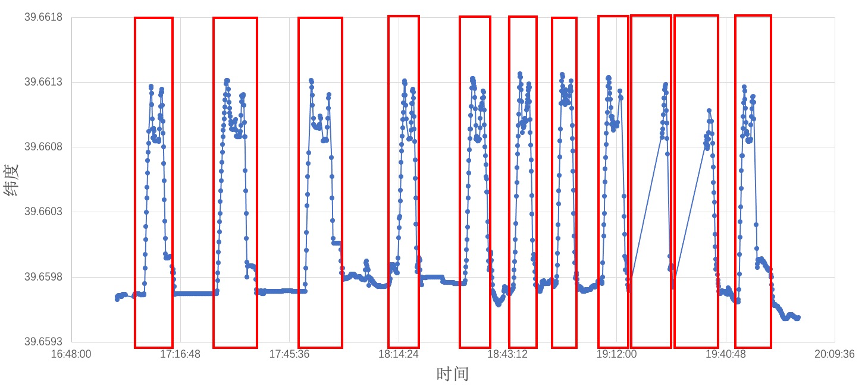
\includegraphics[width=0.86\linewidth]{symmetric_result.png}
  \caption{对称模式挖掘结果}
  \label{fig:symmetric_result}
\end{figure}

\section{时间序列相似性度量}
时间序列对称性的度量,本质上就是时间序列两段子序列的相似性度量。因此,相似性度量算法的选择与研究对于时间序列对称模式挖掘意义重大。现有的时间序列相似性度量方法大体可以划分为两种,一种是基于形状的相似性度量方法,另一种是基于模型的相似性度量方法。下面将围绕这两种方法的国内外研究进行详述。

\subsection{基于形状的相似性度量方法}
在序列相似性度量问题中,欧式距离是一种最为常见的基于距离和形状的方法。对于长度相同的时间序列,通过计算每两点之间的距离然后累积求和,距离越小则相似度越高。这种方法的直观表达可以用式~\ref{eq:euclidean_distance}来表示。
假如$S=\left(\left(t_1,x_1 \right),\left(t_2,x_2\right),\dots,\left(t_n,x_n\right)\right)$
和$Q=\left(\left(t_1,y_1 \right),\left(t_2,y_2\right),\dots,\left(t_n,y_n\right)\right)$是两条时间序列,则这两条时间序列基于欧式距离的相似度则可以用式~\ref{eq:euclidean_distance}来计算
\begin{equation}
  D\left(S,Q\right) = \sqrt{\sum_{i=1}^{n}{\left| x_{i}-y_{i} \right|^{2}}}
  \label{eq:euclidean_distance}
\end{equation}

基于欧式距离的相似性度量方法不仅计算简单、易于理解,计算效率也较高,
当时间序列数据点为多个维度时同样适用。然而,欧式距离要求匹配的两个
时间序列的长度相同,并且由于是一一对应的同步匹配算法,
当出现数据缺失和平移等状况时,会导致欧式距离的度量结果存在很大误差。
例如两个序列$A=\left(2,2,5,5,15,15\right)$和
$B=\left(2,5,5,15,15,15\right)$的欧式距离为109,
然而两个序列的相似度非常高,只是$A$相对于$B$在水平方向上向右发生了平移。

相比于时间序列,字符串相似性的度量方法种类更多,研究更广。因此,
可以采用符号化的表示方法将时间序列转换成字符串序列,
则时间序列相似性度量方法由连续的定量数据的距离度量转换成了离散的
定性数据的距离度量。基于此,Eamonn Keogh和Jessica Lin在2002年
发明了SAX算法,用于将时间序列转换为字符串。
图~\ref{fig:SAX}展示了将时间序列利用SAX符号化为字符串序列的流程,
首先将时间序列数据进行归一化处理,使之具有高斯分布的特征。
然后将新序列降维并用分段聚合近似(PAA)表示,根据使得高斯序列被划分
成任意数量等概率区间的断点序列B,对PAA处理之后的序列完成符号化。
将时间序列传唤未字符串序列之后,字符串距离度量算法相对多样。
接下来将介绍3种经典的字符串距离度量算法。
\begin{figure}
  \centering
  \subcaptionbox{原始时间序列\label{fig:SAX-a}}
    {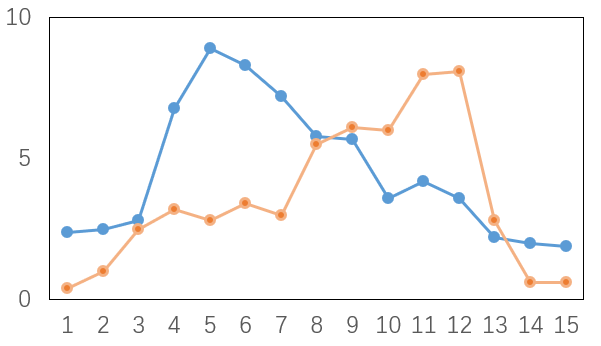
\includegraphics[width=0.43\linewidth]{SAX-a.png}}
  \subcaptionbox{高斯分布归一化处理\label{fig:SAX-b}}
    {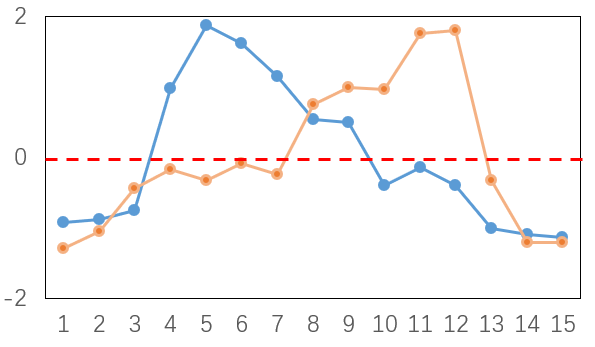
\includegraphics[width=0.43\linewidth]{SAX-b.png}}
  \subcaptionbox{分段聚合近似\label{fig:SAX-c}}
    {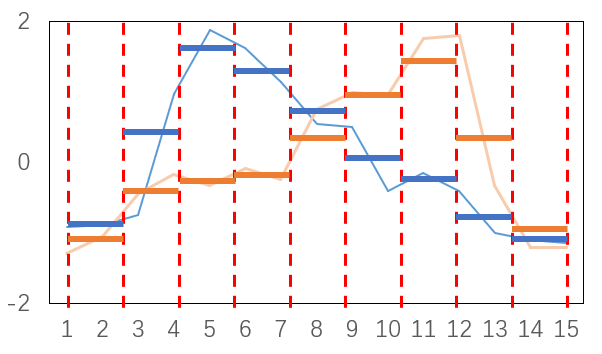
\includegraphics[width=0.43\linewidth]{SAX-c.png}}
  \subcaptionbox{利用断点列表符号化\label{fig:SAX-d}}
    {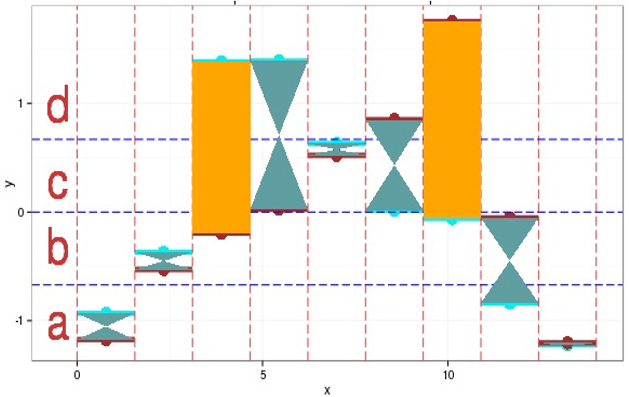
\includegraphics[width=0.43\linewidth]{SAX-d.png}}
  \caption{SAX符号化时间序列算法流程}
  \label{fig:SAX}
\end{figure}

编辑距离原本是对两个字符串差异程度的量化测量,测量方式是计算两个字符串互相转换时需要的最少编辑操作步数,编辑操作包括插入、删除和替换。例如两个序列$A=\left(a,b,c,a,b\right)$和$B=\left(a,c,a,b,b\right)$的编辑距离为2。编辑距离可以通过动态规划的算法思想进行计算,
式~\ref{eq:edit_distance}展示了编辑距离的动态规划方程,当$A$和$B$两个序列的尾字符不相同时,可以通过修改,插入或者删除$A$的尾字符使其与$B$序列相同,从中选择最小值作为序列的编辑距离。


\begin{equation}
  DP(i, j)= \begin{cases}DP(i-1, j-1), & A_{i}=B_{j} \\
    \min \left\{\begin{array}{c}
    D P(i-1, j-1)+1 \\
    D P(i-1, j)+1 \\
    D P(i, j-1)+1
    \end{array}\right. , & A_{i} \neq B_{j}
  \end{cases}
  \label{eq:edit_distance}
\end{equation}

最长公共子序列(LCSS)也可以用来度量两个字符串序列的相似性,
如果一个序列$S$同时是字符串$A$和$B$的子序列。且是所有符合此条件
的最长序列,那么序列S的长度则可以表示两个序列的距离,
并用$S$的长度和$A$、$B$字符串长度最大值的比值衡量两个字符串的相似性。
LCSS也是一种非常经典的利用动态规划思想求解的字符串距离度量算法,
其计算公式如式~\ref{eq:LCSS}所示

\begin{equation}
  D P(i, j)= \begin{cases}0, & i=0 \text { or } j=0 \\ D P(i-1, j-1)+1, & i, j>0 \text { and } A_{i}=B_{j} \\ \max \begin{cases}D P(i-1, j) \\ D P(i, j-1)\end{cases} & i, j>0 \text { and } A_{i} \neq B_{j}\end{cases}
  \label{eq:LCSS}
\end{equation}

除了经典方法,还有一些较为新颖、正处在发展中的字符串距离度量方法,
例如,带惩罚的编辑距离(ERP)方法。ERP算法也是一种基于编辑距离的
字符串距离度量算法。相比经典编辑距离,ERP算法是将匹配过程中插入或删除
时缺少值的一方视为一个gap算子。也就是说,当字符串序列$A$和$B$进行匹配时,
若要在$A_i$插入一个来自$B$序列的$B_j$使得$A$和$B$更为接近时,那么
在距离度量时将不再简单的增加一次编辑操作,而是将$B_j$与$gap$算子的距离视为
本次编辑操作的代价。式~\ref{eq:ERP}展示了ERP方法的计算公式,相比经典编辑距离,
ERP通过指定gap的方式使得距离度量更加灵活,不再是简单编辑操作的数量。
然而,ERP方法的效果和准确率极大的依赖gap的选取,不仅增加了模型的复杂度,
而且不适用于变化剧烈的序列。

\begin{equation}
  D P(i, j)= \begin{cases}\sum_{k=1}^{j}\left|B_{k}-g a p\right|, \qquad \qquad \qquad \qquad \quad i=0 \\
    \sum_{k=1}^{i}\left|A_{k}-g a p\right|,\qquad \qquad \qquad \qquad \quad j=0 \\
    \max \left\{\begin{array}{l}
    \left|A_{i}-B_{j}\right|+D P(i-1, j-1) \\
    \left|A_{i}-\operatorname{gap}\right|+D P(i-1, j) \\
    \left|B_{i}-\operatorname{gap}\right|+D P(i, j-1)
    \end{array}, \quad i, j>0 \text { and } A_{i} \neq B_{j}\right.\end{cases}
    \label{eq:ERP}
\end{equation}

尽管通过符号化的方法将时间序列转化为字符串之后可以通过字符串距离度量
时间序列的相似性,然而,在处理过程中由于降维、平滑和离散化等操作,
必然导致时间序列原始信息的缺失。况且,基于编辑距离的字符串匹配方式
从根本上来说属于部分匹配,通过编辑操作将不匹配的点删除,这种方式度量
出来的距离没有体现全局时间序列的特征。而ERP算法也只是将不匹配点与
一个固定点gap匹配,过于简单粗暴,在不匹配点差距较大时性能下降明显。
而动态时间规整算法(DTW)则是一种直接计算两个时间序列之间相似性的全局
匹配算法。尽管具有相似性的两个时间序列在距离和形状上相近,但是,
由于时间序列的数据维度高,数据类型多样,任何两个序列都有可能存在随机
差异,包括平移伸缩、数据缺失和噪声等。因此,DTW算法并没有拘泥于一对一
的同步匹配方式,而是执行了一对多的异步匹配方式,当存在数据缺失或平移时,
DTW可以从全局匹配的角度为每个点选择最佳匹配。式~\ref{eq:DTW}展示了DTW距离的
计算方式,在时间序列$S=((t_1,x_1 ),(t_2,x_2 ),\dots,(t_n,x_n ))$
和$Q=((t_1,y_1 ),(t_2,y_2 ),\dots,(t_n,y_n ))$的相似性计算过程中,
若$S_i$和$Q_j$点进行匹配,则$S_{i-1}$既可以与$Q_{j-1}$进行匹配,
也可以与$Q_j$进行匹配,同理,$Q_{j-1}$也可以与$S_i$和$S_{i-1}$
进行匹配,从而在保证时间有序性的同时,为每个点尝试所有的匹配可能,
从中选择最佳的匹配方式。因此,DTW度量的相似性不仅可以直接进行连续
时间序列的匹配,还尽量考虑了时许数据的全局性特征,而且对时间序列的
随机性误差具有较高的鲁棒性,是一种较为成熟的时间序列相似性度量方法。
\begin{equation}
  D P(i, j)=D(i, j)+\min \left\{\begin{array}{c}
    D P(i-1, j-1) \\
    D P(i-1, j) \\
    D P(i, j-1)
    \end{array}\right.
    \label{eq:DTW}
\end{equation}

\subsection{基于模型的相似性度量方法}
基于模型的序列相似性度量方法大致可以划分为两大类,一类是基于传统的时间序列预测分析模型的方法,另一类是基于深度学习模型的方法。前者首先对某个时序数据进行模型拟合,然后通过计算利用该模型生成其他时间序列的概率来度量两个时间序列之间的距离和相似性。例如,Ge 等 人利用隐马尔可夫模型(HMM)度量时间序列的相似性,综合考虑了分段线性表示来度量变量之间的相关性和序列的相似性。Panuccio 等人通过标准化处理HMM 的距离分析时间序列模型的拟合性效果。ARIMA(Autoregressive Integrated Moving Average model)模型通过集成自回归和移动平均模型来寻找历史数据之间的自相关性,从而预测未来。对于ARIMA模型而言,可以直接使用模型参数来度量时间序列的相似性。除此之外,还有一些基于特征提取和概率距离的方法,包括Fuchs等人提出的基于正交多项式的时间序列特征表示方法,以及Keogh 等人提出基于统计分布的时间序列概率距离度量模型。

基于深度学习模型的时间序列相似性度量方法的核心思想是利用神经网络将轨迹数据嵌入成低维向量,然后通过度量向量的相似性表示时间序列的相似性。例如,t2vec采用了基于RNN的Seq2Seq结构,其中主要由编码器(encoder)和解码器(decoder)两部分构成,通过学习时间序列的表示向量来缓解时序数据中不一致采样率和噪声对相似度度量的影响。尽管t2vec可以在较高的效率内学习时间序列的模型,但RNN模型在使用过程中会出现误差累积的问题,导致模型对时间序列的预测结果不准。针对此问题,TrjSR通过将轨迹数据表示成为灰度轨迹图像进行解决。
图~\ref{fig:TrjSR}展示了利用TrjSR模型度量时间序列相似性的算法框架,采样率不一致和存在噪声的时间序列数据被表示成为低质量轨迹图像,通过超分辨率成像技术重建出超分辨率轨迹图像后,再被嵌入成低维轨迹向量去计算相似性。
\begin{figure}
  \centering
  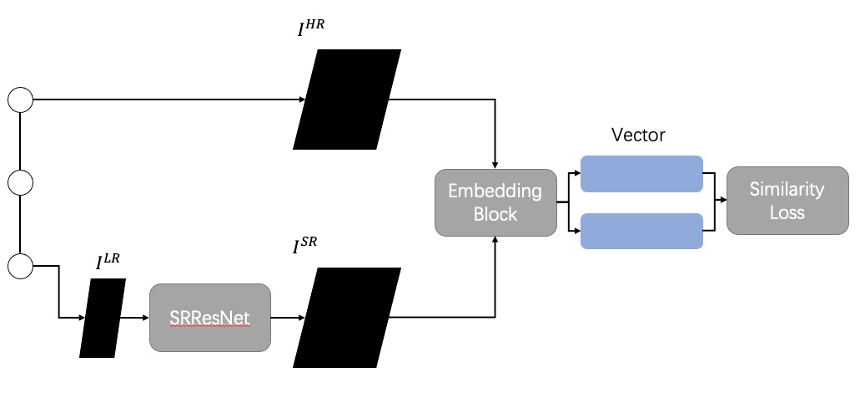
\includegraphics[width=0.86\linewidth]{TrjSR.png}
  \caption{基于TrjSR深度学习模型的时间序列相似性度量}
  \label{fig:TrjSR}
\end{figure}

\section{时间序列模式挖掘}
正如引言所述,随着信息技术的普及和发展,各行各业,尤其是工业领域,通过相应的传感器和信息系统积累了大量的时间序列数据,对特定领域或者特定模式的时间序列数据,利用数学建模、机器学习等方法,进行建模和分析,从而得到特定类型的时间序列子模式,是一项非常有价值的研究课题。本节将针对诸多业内研究者针对时间序列模式挖掘问题提出的多种计算和优化方法进行详述。

\subsection{基于相似性检索的模式挖掘方法}
文本领域中,相似性检索方法在包括社区发现、重复检测、聚类和查询细化都有应用[18,19]。Eamonn Keogh将相似性检索算法扩展到了时间序列领域,通过计算时间序列子序列的全对相似性,识别蕴含在时间序列中的所有模式[4]。该算法使用滑动窗口截取了时间序列的全部子序列,使用归一化的欧几里得距离度量两个时间子序列的距离。为了能加速计算,提升算法的时间效率,该算法被设计成了迭代算法,每次随机抽取一个时间子序列,计算其和全部其他时间子序列的欧几里得距离,从而更新距离最小的时间子序列对的信息。为了利用所有时间子序列中大量的重叠信息,该算法使用离散傅里叶变换算法对原始时间序列进行逆变换,进而计算选中子序列和完整时间序列的距离。该方法具有较强的可扩展性,对于超大规模的数据集,可以随时计算近似结果[20]。

基于相似性检索的模式挖掘方法在对称模式挖掘上具有较大的局限,该方法只能计算出任意两对时间子序列的相似度,却无法判断其是否属于对称子序列。如需挖掘对称模式,当在Matrix Profile算法计算过程中加入子序列对称性的判断,降低算法的时间效率。而且,Matrix Profile算法使用欧氏距离度量两个时间子序列的相似性,由第5章的实验可知,欧几里得距离度量时间序列的相似性忽略了子序列的位置信息从而导致识别不准,在精确率上不如本文设计的对称模式挖掘算法。

\subsection{基于时间序列分解的模式挖掘方法}
在时间序列分析和预测领域,时间序列分解是十分常用的一种方法,
STL(Seasonal-Trend decomposition procedure based on Loess)[19]时间序列分解方法基于LOESS[21]
将某时刻的数据分解为趋势分量,周期分量和余项这三个分量,从而挖掘时间序列中蕴含的周期信息和趋势信息。相比于经典的时间序列分解算法[22],STL并不依赖于移动平均模型,它允许对过程的属性进行分析,对于大量的趋势和季节性的平滑,也可以进行快速计算,并且可以灵活地调整季节项的周期,而不会被数据中的异常行为扭曲。

然而,基于时间序列分解的模式挖掘方法,仅可用于挖掘对称模式为季节模式的时间序列,不能挖掘任意类型的对称模式。真实工业场景中的时间序列数据类型复杂,变化较多,对称模式并不一定呈季节性出现,更可能存在季节性对称模式和非季节性对称模式随机出现的情况。对于该类型的时间序列数据,使用STL算法进行计算往往就不能充分地挖掘出所有的对称模式,或者挖掘出错误的对称模式。

\section{本章小结}
本章定义了论文研究对象的一些相关概念,包括时间序列,对称子序列和对称模式。由于时间序列对称性的度量本质上就是计算时间序列两段子序列的对称性,因此,本章对时间序列相似性度量方法的国内外研究现状进行了分类介绍,主要包括两个类别,即基于形状的相似性度量方法和基于模型的相似性度量方法。其中基于模型的方法不仅增加了复杂性,在实际度量效果中也不如基于形状的方法,其优点只在于可以通过低维向量进行快速检索。因而,本文借鉴基于形状的方法度量时间序列的对称性。由于目前没有成熟的对称模式挖掘算法,本文随后调研了时间序列一般模式挖掘的相关研究。结合模式挖掘和距离度量算法,本文将在后面章节介绍如何在时间序列数据上挖掘对称模式。
% !TeX root = ../thuthesis-example.tex

\chapter{全局对称模式挖掘算法}

本章将对全局对称模式挖掘算法进行研究。根据第2章的定义,
时序数据的全局对称模式指的是所有点关于
某个对称中心前后互为镜像的时间序列。
全局对称模式挖掘就是要通过计算时间序列的对称度,
判断时间序列是否具有对称性。
从数学意义上来说,全局对称模式挖掘算法是分段对称模式挖掘
算法的子问题,全局算法不需要以分段长度$w$作为约束,直接度量
全局的对称性,并以全局对称性在对称度阈值范围内的时间序列整体
做为全局对称模式。
因此,本章节的结构组织如下,在3.1节中分析了
基于对称中心和原始与反转时间序列相似性度量对称性的不足,
进而提出了全局对称模式挖掘算法;在3.2节中根据时间序列的数据特征
分析了对称度阈值确定算法;在3.3节中利用对称度阈值对时间序列进行
分类,从而得到全局对称模式;并在3.4节中将全局对称模式挖掘算法扩展
到了流式数据领域。
% 由两部分构成,分别是全局时间序列对称性度量算法和
% 全局对称度阈值确定算法,本节将分别介绍这两种算法。
% 进一步对所提出的对称模式挖掘方法进行具体阐述。
% 整体来看,时间序列对称模式挖掘分为两大类,
% 一类是时间序列整体组成一个全局的对称模式,
% 另一类是对时间序列进行分段处理,由对称子序列组成的对称模式集合。
% 对于第一类对称模式挖掘,需要一个全局对称性度量算法和
% 基于时间序列数据特征的对称度阈值算法以过滤对称模式。
% 而若需要计算分段时间序列的对称性,
% 则需要在基于分段长度约束的前提下,
% 首先对时间序列进行分段处理,
% 之后通过分段对称性度量算法计算时间子序列的对称度,
% 然后使用由数据特征和对称度分布特征共同确定的对称度阈值
% 分类得到对称子序列,
% 最后根据挖掘数量最多不重叠对称子序列的贪心策略挖掘出对称模式。

在对时间序列的对称度进行度量之前,需要执行一步非常重要的操作,数据归一化。
这是一个在全局对称模式挖掘和分段对称模式挖掘之前都要进行的操作。由于不同来源的时间序列
数据范围往往差距很大,图~\ref{fig:data_range}展示了运输车运输过程中的经度工况时间序列和
有规律心跳过程中力感测电阻器(FSR)信号的变化时间序列,运输车经度的在
(106.89,106.9)范围内,而FSR信号在(-4000,-1000)范围内。
除了范围之外,很明显,两个数据来源的数据跨度差别也很大。
为使用统一的算法框架进行对称模式挖掘,需要对数据进行标准化处理。
对时间序列$X=\left(\left(t_{1}, x_{1}\right),\left(t_{2}, x_{2}\right), \ldots,\left(t_{n}, x_{n}\right)\right)$
的每个数据点,首先根据公式~\ref{eq:mu}计算数据点的平均值,
再根据公式~\ref{eq:sigma}计算数据点的标准差,
最后按照公式~\ref{eq:standard}对时间序列X中所有的数据点进行标准化。
使用z-score方法进行标准化,不仅在无量纲化过程中利用了所有的数据信息,
还消除了各变量在变异程度上的差异,方便提出统一的对称度阈值确定算法。
\begin{equation}
  \mu=\frac{\sum_{i=1}^{i=n} x_{i}}{n}
  \label{eq:mu}
\end{equation}
\begin{equation}
  \sigma=\sqrt[2]{\frac{\sum_{i=1}^{i=n}\left(x_{i}-\mu\right)^{2}}{n}}
  \label{eq:sigma}
\end{equation}
\begin{equation}
  y_{i}=\frac{x_{i}-\mu}{\sigma}
  \label{eq:standard}
\end{equation}
\begin{figure}
  \centering
  \subcaptionbox{挖掘机经度\label{fig:data_range-a}}
  {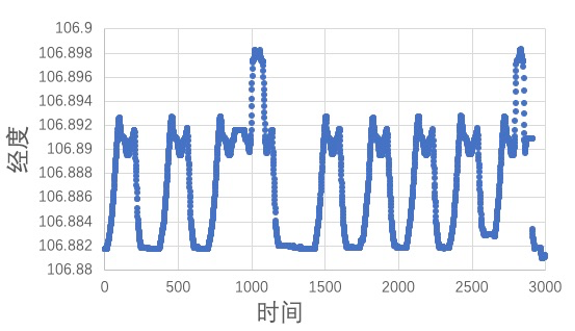
\includegraphics[width=0.43\linewidth]{truck_lo.png}}
  \subcaptionbox{心率FSR信号\label{fig:data_range-b}}
  {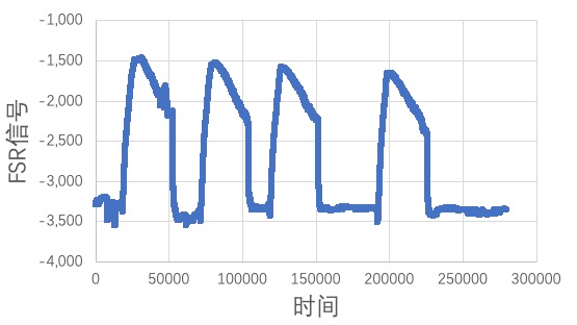
\includegraphics[width=0.43\linewidth]{heart_fsr.png}}
  \caption{不同来源时间序列数据分布范围}
  \label{fig:data_range}
\end{figure}

\section{全局时间序列对称性度量算法}

对于全局时间序列而言,使用原始时间序列和其反转时间序列的相似性来度量对称性,
是一种可行的时间序列对称性度量方法。此方法的好处是可以避免确定对称中心
的问题,但是,这种方法实际上是将时间序列对称中心两侧的子序列进行了
两次匹配,不仅降低了对称性度量算法的时间效率,还增大了对称性的度量结果。
图~\ref{fig:beijing_temp}展示了北京市自1981年至2010年月平均气温的变化,显然,
气温时间序列具有对称性。但是,经计算,原始和反转时间序列的欧式距离为
278.04,而使用本文所提出的对称性度量方法,气温时间序列的对称度仅为
7.6,更加符合真实的时间序列对称性结果。因此,本文定义了一种新的基于
动态时间扭曲算法和区间动态规划思想的对称性
度量方式,既保持了动态时间扭曲算法准确率高、鲁棒性强的特点,
又优化了对称度的计算效率。
\begin{figure}
  \centering
  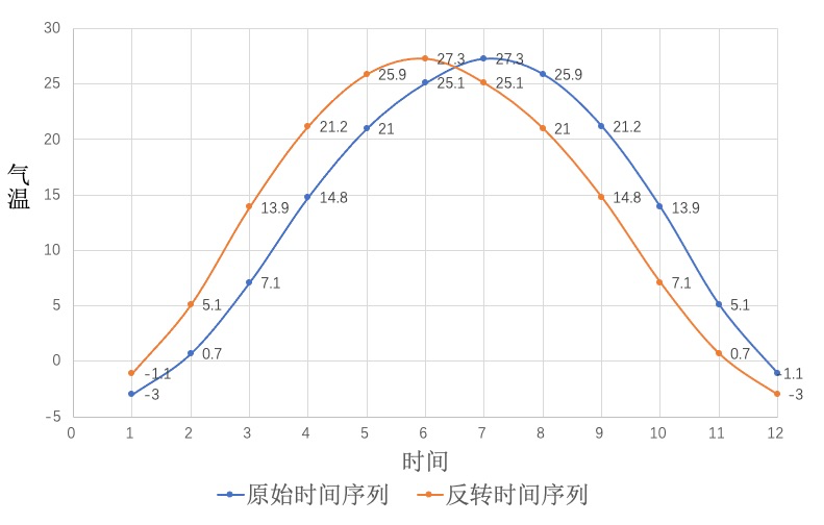
\includegraphics[width=0.86\linewidth]{beijing_temp.png}
  \caption{北京市月平均气温变化}
  \label{fig:beijing_temp}
\end{figure}

首先从全局角度考虑对称时间序列的
匹配过程,由于不存在明确的对称中心,只能通过点和点之间的直接匹配度量
序列的对称性。由于时间序列的采集频率和位置不同,对于每个单点而言,
并不确定最佳匹配点的位置。尽管如此,如果一个时间序列是前后对称的,
那么首尾点一定是匹配的。图~\ref{fig:frontend_match}展示了
对称时间序列匹配过程的候选点,对于时间序列
$X=\left(\left(t_1,x_1 \right),\left(t_2,x_2\right),\dots,
  \left(t_n,x_n \right)\right)$而言,
第一个点$x_1$和最后一个点$x_n$是必然匹配的,但由于时间序列在
同一位置的持续时间不同,其他点如$x_2$和$x_{n-1}$等的匹配点却不是
唯一的,$x_2$可以一一对应地与$x_{n-1}$进行匹配,也可以通过扭曲时间
和$x_n$进行匹配,甚至可以与$x_{n-2},x_{n-3},\dots$等进行匹配,
而制约$x_2$与$x_k$匹配的条件不仅仅是这两点之间的距离,而是
时间序列$\left(\left(t_2,x_2 \right),\dots,\left(t_k,x_k \right)\right)$
的对称度。

\begin{figure}
  \centering
  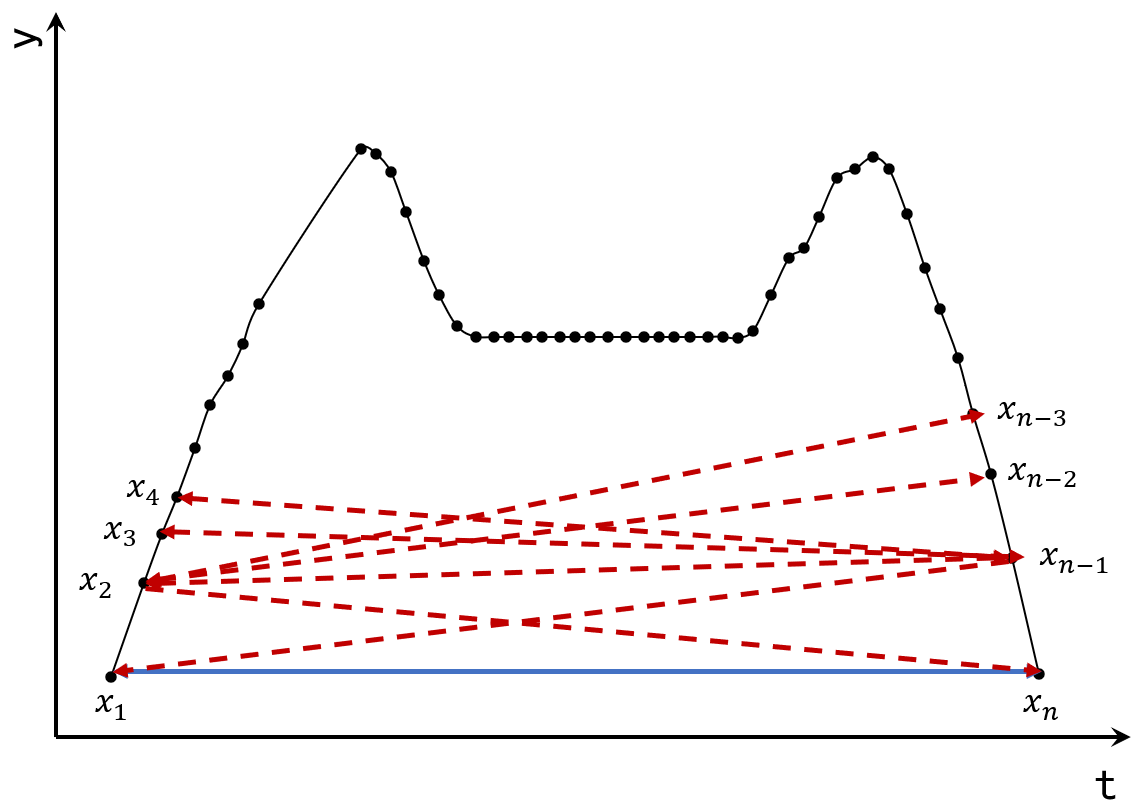
\includegraphics[width=0.76\linewidth]{frontend_match.png}
  \caption{对称时间序列首尾匹配候选点}
  \label{fig:frontend_match}
\end{figure}

接下来,本节将对时间序列的对称度算法进行标准的形式化推导。给定一条时间序列$X=\left(\left(t_1,x_1 \right),\left(t_2,x_2\right),\dots,
  \left(t_n,x_n \right)\right)$,以任意两点间的距离确立$n \times m$的
距离矩阵$D_{n \times m}$,矩阵中的每个元素由公式~\ref{eq:distance_matrix}计算而来
\begin{equation}
  D\left(i, j\right)=\left\|x_{i}-x_{j}\right\|_{w}
  \label{eq:distance_matrix}
\end{equation}

$D\left(i, j\right)$为点$p_i$与$p_j$间的距离,$i,j=1,2,\dots,n$。
显然,点$p_i$和$p_j$的匹配与$p_j$和$p_i$的匹配距离是相同的,
只是匹配顺序不同。为避免重复计算,本文只保留前点和后点的匹配,
则距离矩阵$D_{n \times m}$只需要计算反对角线以上的斜三角矩阵即可。
为了计算$X$的对称度,需要找到一条最优的匹配路径
$R_{best}=\left(r_1,r_2,\dots,r_k \right),\left⌊n/2\right⌋ \leq
  k < n$,使得$X$的累积匹配距离值达到最小, $r_k$表示该匹配路径元素在
距离矩阵中的位置,即$r_k=\left(i,j\right)_k$表示$p_i$与$p_j$之间的匹配关系,
可知$D\left(r_k \right)=D\left(i,j\right)_k$一般存在着多条匹配路径,
有效的弯曲路径$R$必须符合以下3个条件:
\begin{enumerate}
  \item 边界性:$r_{1} \in\{(i, i),(i, i+1) \mid 1 \leq i \leq n\}, \quad r_{k}=(1, n)$
  \item 单调性:给定$r_{k}=(i, j)$和$r_{k+1}=\left(i^{\prime}, j^{\prime}\right), \quad i^{\prime} \leq i, j^{\prime} \geq j$
  \item 连续性:给定$r_{k}=(i, j)$和$r_{k+1}=\left(i^{\prime}, j^{\prime}\right), \quad i^{\prime} \geq i-1, j^{\prime} \leq j+1$
\end{enumerate}

边界性是确保$R$的起点$r_1$在相似度矩阵的反对角线或者相邻斜线上,
而终点$r_k$在矩阵的右上角$\left(1,n\right)$。
单调性和连续性是为了保证匹配路径的下一个点在当前点的上方、右上方或右方。
在所有有效的路径中, 找到唯一且最优的路径使得累积匹配距离和达到最小,
公式~\ref{eq:best_route}即为优化目标:
\begin{equation}
  D(X)=\min \left\{\sum_{k=1}^{K} D\left(r_{k}\right)\right\}
  \label{eq:best_route}
\end{equation}

\begin{figure}
  \centering
  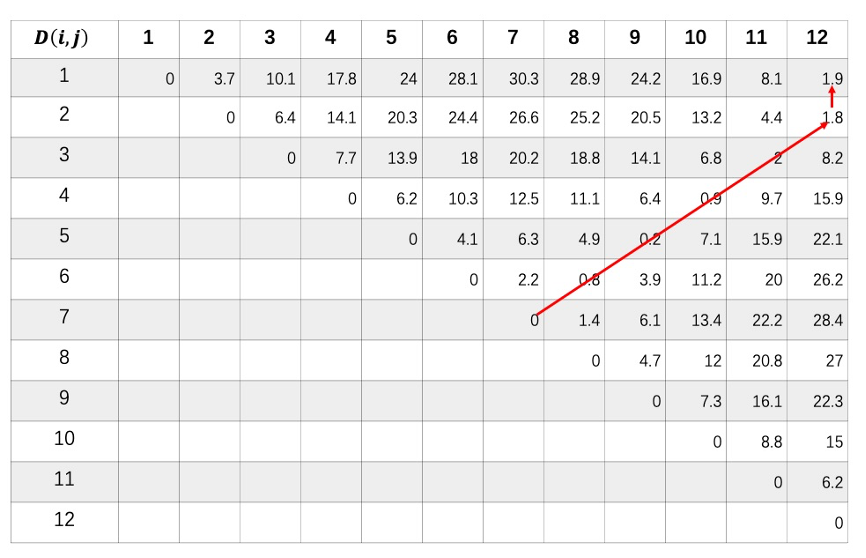
\includegraphics[width=0.86\linewidth]{symmetric_matrix.png}
  \caption{相似度矩阵最优匹配路径示意图}
  \label{fig:symmetric_matrix}
\end{figure}

然而,从$r_1$到$r_k$的有效路径却是指数级的,采用暴力求解的方法不现实。
图~\ref{fig:symmetric_matrix}展示了一个时间序列在对称度矩阵上的最优
匹配路径。观察发现,路径R中的点$r_i$对于时间序列而言是由内向外匹配的。
如果$r_{k+1}$与$r_k=\left(i,j\right)$属于同一个匹配路径中的相邻点,
则$r_{k+1}$只有$(i-1, j),(i-1, j+1),(i, j+1)$这三种可能,
即$r_{k+1}$所表示的匹配范围正好包含了$r_k$的匹配范围,这种匹配顺序
符合了动态规划推导思想的无后效性。进一步,如果约定$D P(i, j)$表示时间序列
$X$的子序列$S=\left(p_{i}, p_{i+1}, \dots, p_{j}\right)$的对称度,
则该状态可以由$\{D P(i+1, j), D P(i, j-1), D P(i+1, j-1)\}$中
最小的一个推导而来,这种小区间和大区间的状态具有严格单调性的模型非常
符合区间动态规划算法思想。因此,为了求解式~\ref{eq:best_route},
利用区间动态规划方法构造一个代价矩阵$DP$, 其中每个元素通过式~\ref{eq:dp_item}得到:
\begin{equation}
  D P(i, j)=D(i, j)+\min \left\{\begin{array}{c}
    D P(i+1, j) \\
    D P(i, j-1) \\
    D P(i+1, j-1)
  \end{array}\right.
  \label{eq:dp_item}
\end{equation}

其中:$1 \leq i \leq j \leq n, D P(i, i)=0, D P(i, i+1)=D(i, i+1)$。
式~\ref{eq:dp_item}表示当前区间的匹配累积距离等于当前点的距离值加上紧邻
3个区间匹配累积距离的最小值,$D P(1, n)$便是时间序列X的最小匹配累积
代价,即对称度。得到对称度后, 为了得到最优匹配路径,
再反向以$r_k$为起点寻找匹配路径。直到$i=j$或者$i=j-1$时,
寻找过程结束,最终得到完整的匹配路径。通过累积计算匹配路径中每对匹配点之间的距离,
可以得到匹配点的距离之和,最终计算得到的$DP(1,n)$即可视为时间序列$X$的对称度。

\renewcommand{\algorithmicrequire}{\textbf{输入:}\unskip}
\renewcommand{\algorithmicensure}{\textbf{输出:}\unskip}

\begin{algorithm}
  \caption{全局时间序列对称性度量算法$calculate\_global\_symmetry$}
  \label{alg:global_symmetry}
  \small
  \begin{algorithmic}
    \REQUIRE 时间序列$X=\left(p_{1}, p_{2}, \dots, p_{n}\right)$
    \ENSURE 对称度$d$

    \STATE $n \leftarrow \left|X\right|$
    \STATE $i \leftarrow 1$
    \WHILE{$i \leq n$}
    \STATE $dp_{i,i} \leftarrow inf$
    \ENDWHILE

    \STATE $i \leftarrow 1$
    \WHILE{$i < n$}
    \STATE $dp_{i,i+1} \leftarrow D\left(p_{i}, p_{i+1}\right)$
    \ENDWHILE

    \STATE $len \leftarrow 3$
    \WHILE{$len \leq n$}
    \STATE $i \leftarrow len$
    \WHILE{$i \leq n-len+1$}
    \STATE $dp_{i,i+len-1} = D\left(p_{i}, p_{i+1}\right)+\min \left(dp_{i,i+len-2},dp_{i+1,i+len-1},dp_{i+1,i+len-2}\right)$
    \ENDWHILE
    \ENDWHILE
    \RETURN $dp_{1,n}$
  \end{algorithmic}
\end{algorithm}

算法~\ref{alg:global_symmetry}给出了
全局时间序列对称性度量算法的计算流程。
第1-9行初始化计算长度为1和2的时间子序列对称度,
第10-17行根据式~\ref{eq:dp_item}所示的区间动态规划算法
度量得到时间序列的全局对称度。

总结来说,本方法利用区间动态规划的算法思想,提出了一种兼顾距离相近和形状相似的时间序列对称性
度量方法,既避免了时间序列对称中心不固定带来的匹配问题,也通过异步匹配
提高了度量的准确性和健壮性,同时,因减少了重复匹配,也提高了本算法的
时间效率。尽管其渐进时间复杂度仍然为$O\left(w^{2}\right)$,
但相比于基于原始和反转时间序列的DTW距离的相似度度量算法,
减少了$50 \%$的重复匹配,提升了时间序列对称度的计算效率。

\section{全局对称度阈值确定算法}

3.1节讲述了时间序列的全局对称性度量算法,在得到全局时间序列的
对称度之后,还需要确定对称度阈值,才能判断时间序列是否具有对称性。
对称度阈值用于对时间序列进行分类,
对称度在阈值范围内的序列划分为对称模式,否则划分为非对称模式。
在真实工业场景的数据挖掘中,经常由专家根据领域知识人为确定
先验阈值。例如,在运输车行驶往返形成的时间序列数据中,
由于车道变换导致的相同位置经度变化不会超过0.0001度,
此经验信息可以用为对称模式匹配过程中的单点匹配误差阈值。
尽管使用经验阈值的方式可以高效的对时间序列对称模式进行分类,
但并不是所有来源的数据集都有明确的经验阈值,或者其阈值
只是一个较为模糊的范围,不具有进行对称模式分类的作用。
因此,需要设计一种不依赖于领域知识的对称度阈值确定算法。

考虑到对称度本质上是时间序列前后匹配得到的
自相似性结果,因此,对称度阈值必然和时间序列本身的
差异程度密切相关。如果时间序列的变化比较平缓,为了将对称模式
挖掘出来,对称度阈值就需要设定的较小。
如果时间序列变化特别剧烈,相应的在进行对称时间序列匹配的过程中,
匹配点的差异可能就特别大,因此,对称度阈值也需要
设定的较大。然而,影响对称度阈值高低的关键因素不是标准差
代表的整体时间序列的差异程度,而是匹配点之间的差异程度。
图~\ref{fig:symmetry_diff}展示了标准化后正弦曲线和
河北某县气温的变化时间序列,
两者都是对称时间序列。然而,尽管两者的标准差都是1,
但因为正弦时间序列完美匹配而气温时间序列匹配存在误差,
所以前者的对称度为0,而后者的对称度为0.7。
\begin{figure}
  \centering
  \subcaptionbox{标准化正弦时间序列\label{fig:symmetry_diff_sin}}
  {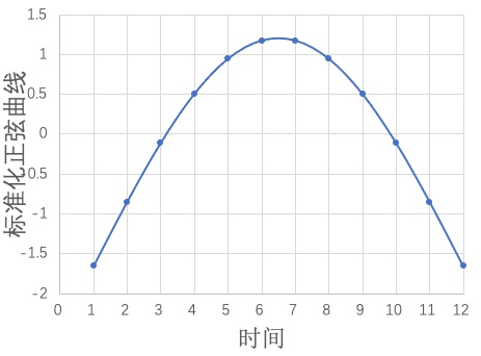
\includegraphics[width=0.43\linewidth]{symmetry_diff_sin.png}}
  \subcaptionbox{标准化气温时间序列\label{fig:symmetry_diff_temp}}
  {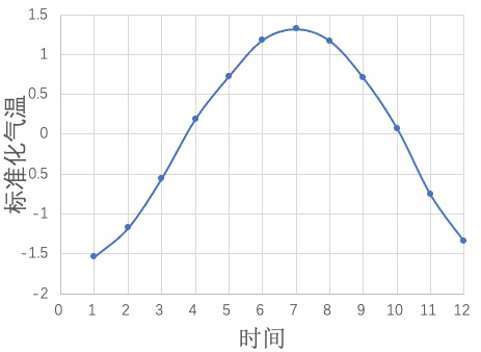
\includegraphics[width=0.43\linewidth]{symmetry_diff_temp.png}}
  \caption{不同来源对称时间序列对称度差异}
  \label{fig:symmetry_diff}
\end{figure}

因此,要根据时间序列点匹配的情况确定对称度阈值。然而,
根据时间序列匹配点之间的距离确定对称阈值具有极大的随机性。
对称度阈值的选取将极大地受对称性度量算法的影响。
因为对称性度量算法将决定时间序列点的匹配位置。
这样得到的对称度阈值不具有统一性,算法也不具备可迁移性。因此,
对称度阈值的确定还是需要立足时间序列本身的数据特征。
本文使用在同一个时间序列中前后相邻点的
差距作为确定对称度阈值的参考。因为对称时间序列要求前后点相匹配,
符合要求的匹配应该满足匹配点对的距离尽可能小,进而也尽量不要超过匹配点
的近邻点。因此,近邻点距离的统计指标对于判断全局对称模式
具有很重要的参考意义。
相比中位数,近邻点距离的平均数更能反映时间序列的整体变化程度,
也更适用于对利用全局对称性度量算法计算出来的时间序列对称度进行分类。
因为中位数只是考虑了相邻点距离在分布上的中间位置情况,
并未考虑可能存在的距离较大的近邻点。而全局对称性度量算法
是从时间序列全局为每个点寻找最佳匹配点,可能包含部分匹配
偏差较大的点,其最终得到的单点对称度从数学意义上来说也是
全局匹配点距离的平均数。因此,可以使用式~\ref{eq:threshold1}
所表示的时间序列近邻点距离的平均值,作为全局时间序列对称模式挖掘
算法的对称度阈值。为与第4章提出的分段对称度阈值进行区分,
全局对称度阈值用$\theta_1$来表示。
对称度阈值需要统一量纲,由于不同来源时间序列对称模式的长度不一致,
因而经全局时间序列对称性度量算法计算出来的对称度
也要求其与对称模式长度的比值。
\begin{equation}
  \theta_{1}=\frac{\sum_{i=2}^{n}\left|x_{i}-x_{i-1}\right|}{n-1}
  \label{eq:threshold1}
\end{equation}

\section{挖掘全局对称模式}
通过全局对称性度量算法计算得到时间序列的对称度之后,就可以
使用领域知识和自定义算法确定的对称度阈值对模式进行分类。
在未指定先验阈值的情况下,如果根据公式~\ref{eq:threshold1}
计算得到的对称度阈值为$\theta_1$,那么,本文所要挖掘的对称模式
即是满足公式~\ref{eq:global_symmetry}的时间序列。
\begin{equation}
  S = \{X|D(X)\leq\theta_1\}
  \label{eq:global_symmetry}
\end{equation}

综上所述,全局时间序列对称模式挖掘的计算步骤如算法~\ref{alg:global_symmetric}
所示。首先使用全局对称性度量算法计算时间序列的
对称度,之后由公式~\ref{eq:threshold1}
计算时间序列数据特征相关的对称度阈值,
最后通过比较时间序列的对称度是否在阈值范围内
确定其是否属于全局对称模式。

\renewcommand{\algorithmicrequire}{\textbf{输入:}\unskip}
\renewcommand{\algorithmicensure}{\textbf{输出:}\unskip}
\begin{algorithm}
  \caption{全局对称模式挖掘算法$calculate\_global\_symmtric\_pattern$}
  \label{alg:global_symmetric}
  \small
  \begin{algorithmic}
    \REQUIRE 时间序列$X=\left(p_{1}, p_{2}, \dots, p_{n}\right)$
    \ENSURE 布尔型变量,标志全局时间序列$X=\left(p_{1},p_{2},…,p_n \right)$是否为全局对称模式

    \STATE $d \leftarrow calculate\_global\_symmetry(X) $
    \STATE $i \leftarrow 1$
    \WHILE{$i < \left|X\right|$}
    \STATE minus $\leftarrow$ minus $+D\left(p_{i}, p_{i+1}\right)$
    \STATE $i \leftarrow i+1$
    \ENDWHILE
    \STATE $\theta_1 \leftarrow frac{minus}{n-1}$
    \IF{$d \leq \theta_1 $}
      \RETURN true
    \ELSE
      \RETURN false
    \ENDIF
  \end{algorithmic}
\end{algorithm}


\section{全局对称模式流式挖掘算法}
在实际场景中,经常有在对称模式发生时即时报警的应用。
金融市场和股票分析是一个对数据的实时性要求很高的场景,
如果在股票指数或价格时间序列出现符合某种模式的特征时能及时预报,
将具有极大的应用价值。图~\ref{fig:shanghai_point}展示了
上证指数在2005年至2015年的变化时间序列,
红框所示曲线符合对称模式特征。股票市场中的对称理论是一个
比较小众但成熟的理论,总结为三大对称定律:
其一为价格对称,即股票上涨的价格和下跌的价格相同;
其二为时间对称,股票上涨持续的时间与下跌持续的时间一致;
其三为高低对称,即股票上涨到一半时,后段的走势与前段的走势呈对称状。
这些定律非常符合本文提出的时间序列对称模式特征。
金融时间序列中的对称模式意味着当前经济周期的结束,
如果能成功识别对称模式,在某种意义上则可以成功预测股票的走势,
在经济周期中获得经济效益。然而,金融时间序列往往都有很强的实时性,
数据是实时更新的,不具备第3.1节中已知全局时间序列的情况。
并且,金融时间序列变化快速且剧烈,因此要求算法能快速响应。
基于此,本节通过优化全局对称模式挖掘算法的状态推导,
提高了算法的时间效率,将其扩展到了流式应用场景。
\begin{figure}
  \centering
  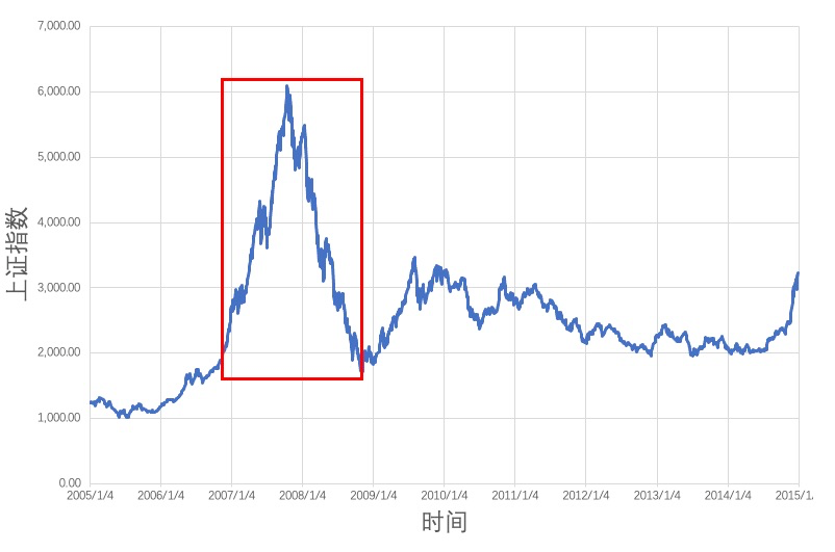
\includegraphics[width=0.86\linewidth]{shanghai_point.png}
  \caption{上证指数自2005年至2015年单日变化情况}
  \label{fig:shanghai_point}
\end{figure}

\subsection{流式时间序列对称性度量}
流式时间序列是一组顺序、大量、快速且连续到达的时间序列数据。
一般情况下,时间序列数据流可被视为一个随时间延续而无限增长的
动态数据集合。如果能够随着数据点的到来,
不断地对之前所有数据点组成的流式时间序列度量对称性,并在
对称度超过阈值时及时报警,则算法在实时计算领域具有重要的应用价值。
检测流式时间序列的对称性需要满足实时性和高效性,
即给定一个实时生成的时间序列$X=(p_1,p_2,\dots,p_t)$,
需要在每个数据点$p_t$生成时,以较高的效率
而不是重新计算的方式检测并度量全局流式时间序列$X$的对称性。
由3.1节可知,使用$DP\left(1,t-1\right)$表示流式时间子序列
$S=(p_1,p_2,\dots,p_{t-1} )$的对称度。因此,
当新到来一个数据点$p_{t}$时,可以用公式~\ref{eq:stream_dp}
计算$DP\left(1,t\right)$。然而在该公式中,
由于$p_{t}$是新增点,状态$DP\left(2,t\right)$
尚未计算,不可直接使用。若直接用DTW算法计算全局流式时间序列$X$
与其反转序列的DTW距离作为该序列的对称度,不仅使得对称度结果
偏高,且其时间复杂度又退化为$O\left(t^2\right)$。
因此,需要考虑如何利用已计算的状态优化流式算法。
\begin{equation}
  DP(1, t)=D(1, t)+\min \left\{\begin{array}{c}
    D P(2, t) \\
    D P(1, t-1) \\
    D P(2, t-1)
    \end{array}\right.
  \label{eq:stream_dp}
\end{equation}

图~\ref{fig:latitude_stream_matrix}展示了运煤车单次运输过程中纬度变化时间序列和
单点实时新增时对称度状态推导的变化过程,通过观察动态规划状态
的推导过程可知,当新增一个数据点$p_t$时,流式时间子序列
$S=\left(p_{1},p_{2},…,p_{t-1} \right)$
范围之内的对称度状态不须重新推导。因为根据3.1节介绍的时间序列
对称模式挖掘算法的数学性质,该算法满足单调性和连续性,时间序列
$S$从$p_{1}$到$p_{t-1}$之间的对称度状态$DP\left(i,j\right)$
仍然是由$DP\left(i+1,j\right)$,$DP\left(i,j-1\right)$
和$DP\left(i+1,j-1\right)$推导而来。这三个状态在对称度矩阵
中分别位于$DP\left(i,j\right)$的下方、左方和左下方。
而由图~\ref{fig:latitude_stream_matrix}的状态转移矩阵可知,
当新增数据点$p_t$时,对称度状态矩阵窗口
整体向右下方扩张,并未导致$p_{1}$到$p_{t-1}$之间产生
状态失效,这就使得对称度矩阵内的状态推导顺序仍然有效。并且,
对称度模式挖掘算法的起始状态是两点间距离,也不会随着新数据点的
到来而发生改变。在推导顺序和起始状态均未改变的前提之下,只需
计算$DP\left(k,t\right),1\leq k \leq t$,
即图~\ref{fig:latitude_stream_matrix}所示状态转移矩阵的
最后一列状态即可。由状态转移矩阵的转移路径可知,
只需在$O\left(t\right)$的时间内便可计算出$DP\left(k,t\right)$,
相比通过计算原始和反转时间序列的相似性度量对称性的算法大大降低了时间复杂度。
\begin{figure}
  \centering
  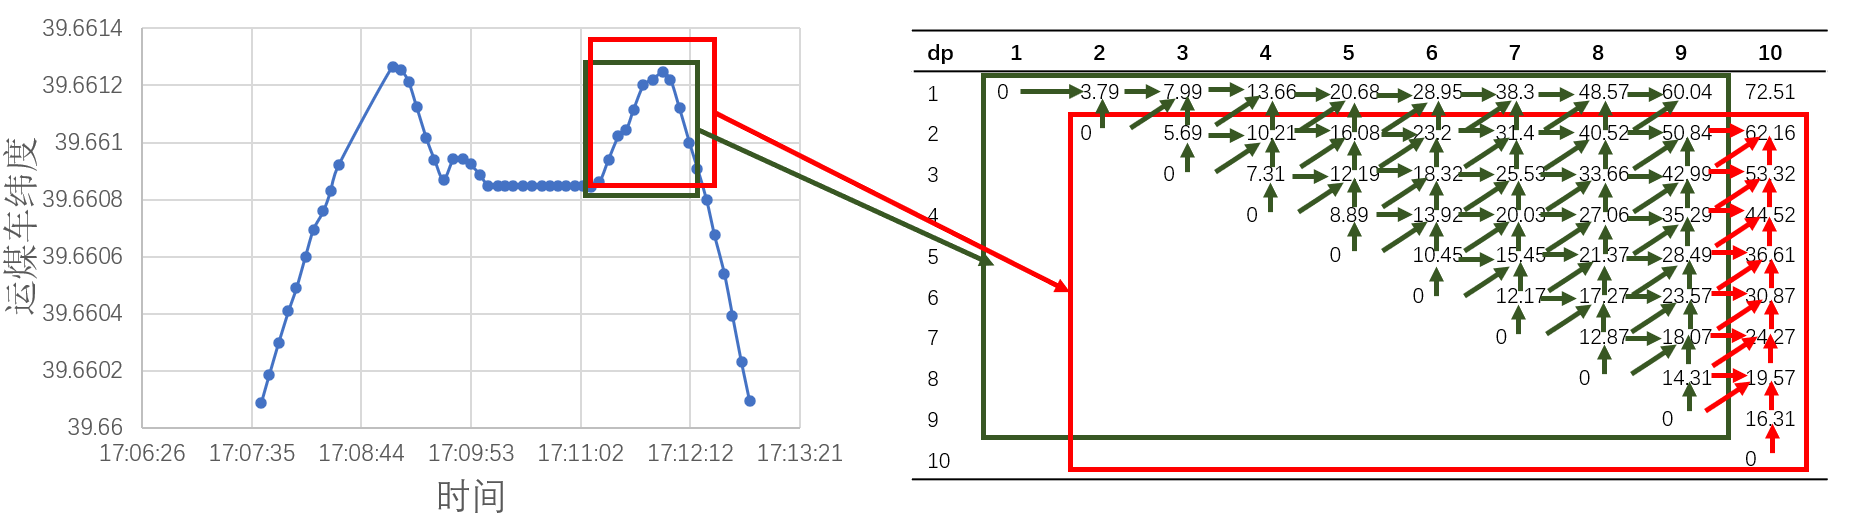
\includegraphics[width=0.86\linewidth]{latitude_stream_matrix.png}
  \caption{运煤车纬度变化与对称度状态转移过程}
  \label{fig:latitude_stream_matrix}
\end{figure}

\subsection{流式挖掘全局对称模式}
本节根据上述对称模式挖掘方法在流式数据上的分析和扩展,
提出了相应的流式挖掘算法。在流式应用场景中,
触发计算的是新数据点的到达,其他位于窗口内的数据点已经到达
并保存。因此,需要自定义并维护一个队列保存流式时间序列$X$,
由历史已经到达的数据点组成,作为流式计算的
状态信息。并且,由图~\ref{fig:latitude_stream_matrix}的
状态转移矩阵可以发现,流式全局对称模式挖掘算法并不需要利用
完整的对称度矩阵信息,当新增一个数据点$p_t$时,只需要用到
对称度矩阵的最后一列状态来推导和$p_t$相关的状态。
因此,可以使用一维列表$dp$作为保存对称度矩阵的数据结构,
在利用以点$p_{t-1}$为结束点的旧有$dp$计算得到新数据点
$p_t$的相关状态后,用新计算得到的$dp$更新旧有$dp$即可,
进而优化空间复杂度。
此外,由于流式数据是动态、源源不断到来的,模式识别需要实时报警。
因此,可以采用全局对称度阈值确定算法对流式全局对称模式进行分类。
总之,对称模式流式挖掘算法只需要
新增数据点$p_t$作为输入,同时保存
流式全局时间序列$X$,流式对称度状态列表$dp$和
流式全局对称度阈值$\theta_1$作为状态信息,
对于所有的流式全局时间序列$X$,比较其对称度和阈值的数量关系,
输出其是否属于全局对称模式。

算法~\ref{alg:streaming_symmetric_pattern}
展示了时间序列对称模式流式挖掘算法
的计算流程,第1-16行在$O(t)$的时间内
流式计算以与点$p_t$相关的全局对称度状态$dp$,
并更新对称度阈值$\theta_1$,
第17行把新数据点放入流式时间序列$X$,
第18-22行
并通过比较流式全局对称度是否超过对称度阈值,判断是否为对称模式。
分析可知,当每个新数据点到来时,
全局对称模式流式挖掘算法的时间和空间复杂度均为$O(t)$,
远远低于每次都重新计算DTW距离以度量对称性的算法,
具有较高的时间效率和较快的响应速度。
此外,根据第4章的研究,流式挖掘算法很容易扩展到分段对称模式挖掘领域,
在结合IoTDB系统实现时具有重要的应用价值。

\renewcommand{\algorithmicrequire}{\textbf{输入:}\unskip}
\renewcommand{\algorithmicensure}{\textbf{输出:}\unskip}

\begin{algorithm}
  \caption{全局对称模式流式挖掘算法$calculate\_streaming\_symmtric\_pattern$}
  \label{alg:streaming_symmetric_pattern}
  \small
  \begin{algorithmic}
    \REQUIRE 新数据点$p_t$
    \ENSURE 布尔型变量,标志流式全局时间序列$X=\left(p_{1},p_{2},…,p_t \right)$是否为流式全局对称模式

    \IF{$t = 1$}
      \STATE $dp_{1} \leftarrow 0$
    \ELSE
      \STATE $\theta_1 \leftarrow \theta_1+D\left(p_{t}, p_{t-1}\right)$
      \STATE $dp_1^{\prime} \leftarrow 0$
      \STATE $ idx \leftarrow 1$
      \WHILE{$ idx \leq |dp|$}
        \STATE $ idx \leftarrow idx+1$
        \IF{$idx = 2$}
          \STATE $dp_{idx}^{\prime} \leftarrow D\left(p_{t}, p_{t-idx-1}\right)$
        \ELSE
          \STATE $dp_{idx}^{\prime} \leftarrow D\left(p_{t}, p_{t-idx-1}\right)+min(dp_{idx},dp_{idx-1},dp_{idx-1}^{\prime})$
        \ENDIF
      \ENDWHILE
      \STATE $ dp \leftarrow dp^{\prime}$
    \ENDIF
    \STATE 将$p_t$置于流式时间序列$X$中
    \IF{$\frac{dp_{t}}{w} > \frac{\theta_1}{w-1}$}
      \RETURN false
    \ELSE
      \RETURN true
    \ENDIF
  \end{algorithmic}
\end{algorithm}

\section{本章小结}
本章主要介绍了全局时间序列对称模式挖掘的整体框架和算法细节。
首先定义了对于完整的全局时间序列如何度量对称性,根据全局最优匹配
和区间动态规划的算法思想设计了全局对称性度量算法。然后,
在先验阈值可能缺省的前提下,3.2节通过分析时间序列
数据特征,根据数据点差分距离的平均值确定了全局对称度阈值。
并在3.3节利用全局对称度阈值过滤得到了全局对称模式。
最后,本文通过优化对称度计算方式
将全局对称模式挖掘算法扩展到了流式数据领域。
根据第5章的实验证明,本节所定义的全局对称模式挖掘算法
在不同来源的数据集上具有更高的准确性和鲁棒性。
% !TeX root = ../thuthesis-example.tex

\chapter{对称模式挖掘算法的扩展}
本章将研究对称模式挖掘算法在复杂应用场景中的扩展。首先介绍了对称模式挖掘算法在大规模流式数据中的扩展。通过分析当前算法在流式数据中的不足之处,对区间动态规划状态进行优化,采用以空间换时间的策略提高对称模式挖掘算法在流式数据中的时间效率。然后分析了时间序列中存在多种对称模式给模式挖掘带来的困难,通过提出算法自适应的调整窗口大小,提高了对称模式挖掘的完整性。综合来看,通过调整对称模式挖掘的模型约束,可以很方便的将对称模式扩展到其他领域的应用场景。

\section{对称模式流式挖掘算法的设计与实现}
在实际场景中,经常有在对称模式发生时即时报警的应用。金融市场和股票分析是一个对数据的实时性要求很高的场景,如果在股票指数或价格时间序列出现符合某种模式的特征时能及时预报,将具有极大的应用价值。
图~\ref{fig:shanghai_point}展示了上证指数在2005年至2015年的变化时间序列,红框所示曲线符合对称模式特征。股票市场中的对称理论是一个比较小众但成熟的理论,总结为三大对称定律:其一为价格对称,即股票上涨的价格和下跌的价格相同;其二为时间对称,股票上涨持续的时间与下跌持续的时间一致;其三为高低对称,即股票上涨到一半时,后段的走势与前段的走势呈对称状。这些定律非常符合本文提出的时间序列对称模式特征。金融时间序列中的对称模式意味着当前经济周期的结束,如果能成功识别对称模式,在某种意义上则可以成功预测股票的走势,在经济周期中获得经济效益。然而,金融时间序列往往都有很强的实时性,数据是实时更新的,不具备第3节已知全局时间序列的情况。并且,金融时间序列变化快速且剧烈,因此,要求算法能快速响应。基于此,本节通过优化对称模式挖掘算法的状态推导,提高了算法的时间效率,将其扩展到了流式应用场景。
\subsection{流式对称子序列计算}
流式时间序列是一组顺序、大量、快速且连续到达的时间序列数据。
一般情况下,时间序列数据流可被视为一个随时间延续而无限增长的
动态数据集合。检测流式时间序列的对称性需要满足实时性和高效性,
即给定一个实时生成的时间序列$X=(p_1,p_2,\dots)$和时间窗口$w$,
需要在每个数据点$p_t$生成时,检测并度量时间子序列
$S=\left(p_{t-w+1},p_{t-w+2},\dots,p_t \right)$的对称性。
\begin{figure}
  \centering
  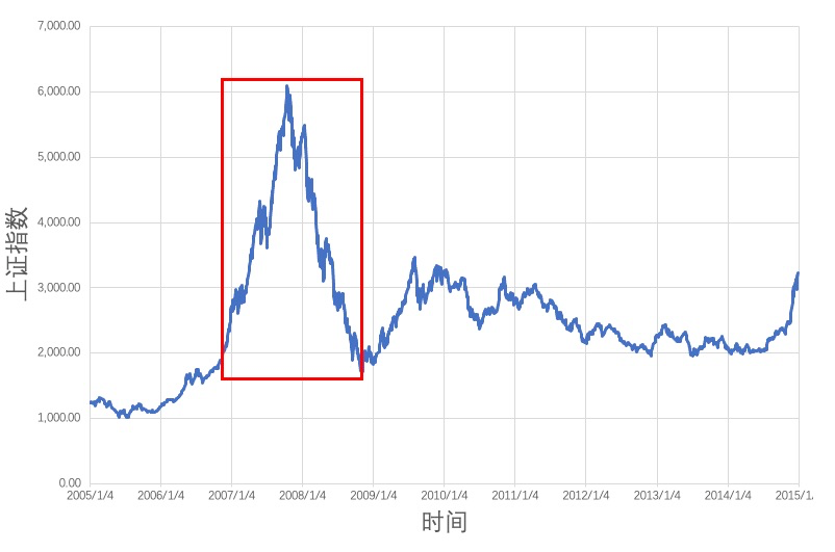
\includegraphics[width=0.86\linewidth]{shanghai_point.png}
  \caption{上证指数自2005年至2015年单日变化情况}
  \label{fig:shanghai_point}
\end{figure}
由3.1节可知,使用$DP\left(i,j\right)$表示时间序列
$Q=(p_i,p_{i+1},\dots,p_j )$的对称度。因此,
当新到来一个数据点$p_(j+1)$时,可以用公式~\ref{eq:stream_dp}
计算$DP\left(i+1,j+1\right)$。然而在该公式中,
由于$p_(j+1)$是新增点,状态$DP\left(i+2,j+1\right)$
尚未计算,不可直接使用。若直接用DTW算法计算
$S=\left(p_{t-w+1},p_{t-w+2},…,p_t \right)$
与其反转序列的DTW距离作为该序列的对称度,不仅使得对称度结果
偏高,且其时间复杂度又退化为$O\left(w^2\right)$。
因此,需要考虑如何利用已计算的状态优化流式算法。
\begin{equation}
  DP(i+1, j+1)=D(i+1, j+1)+\min \left\{\begin{array}{c}
    D P(i+2, j+1) \\
    D P(i+1, j) \\
    D P(i+2, j)
    \end{array}\right.
  \label{eq:stream_dp}
\end{equation}

图~\ref{fig:latitude_stream_matrix}展示了运煤车单次运输过程中纬度变化时间序列和
单点实时新增时对称度状态推导的变化过程,通过观察动态规划状态
的推导过程可知,当新增一个数据点$p_t$时,时间子序列
$S=\left(p_{t-w+1},p_{t-w+1},…,p_{t-1} \right)$
范围之内的对称度状态不须重新推导。因为根据3.1节介绍的时间序列
对称模式挖掘算法的数学性质,该算法满足单调性和连续性,时间序列
$S$从$p_{t-w+1}$到$p_{t-1}$之间的对称度状态$DP\left(i,j\right)$
仍然是由$DP\left(i+1,j\right)$,$DP\left(i,j-1\right)$
和$DP\left(i+1,j-1\right)$推导而来。这三个状态在对称度矩阵
中分别位于$DP\left(i,j\right)$的下方、左方和左下方。
而由图~\ref{fig:latitude_stream_matrix}的状态转移矩阵可知,
当新增数据点$p_t$时,对称度状态矩阵窗口
整体向右下方移动,并未导致$p_(t-w+1)$到$p_(t-1)$之间产生
状态失效,这就使得对称度矩阵内的状态推导顺序仍然有效。并且,
对称度模式挖掘算法的起始状态是两点间距离,也不会随着新数据点的
到来而发生改变。在推导顺序和起始状态均未改变的前提之下,只需
计算$DP\left(k,j+1\right),i+1\leq k \leq j+1$,
即图~\ref{fig:latitude_stream_matrix}所示状态转移矩阵的
最后一列状态即可。由状态转移矩阵的转移路径可知,
只需在$O\left(w\right)$的时间内便可计算出$DP\left(k,j+1\right)$,
相比通过计算原始和反转时间序列的相似性度量对称性的算法大大降低了时间复杂度。
\begin{figure}
  \centering
  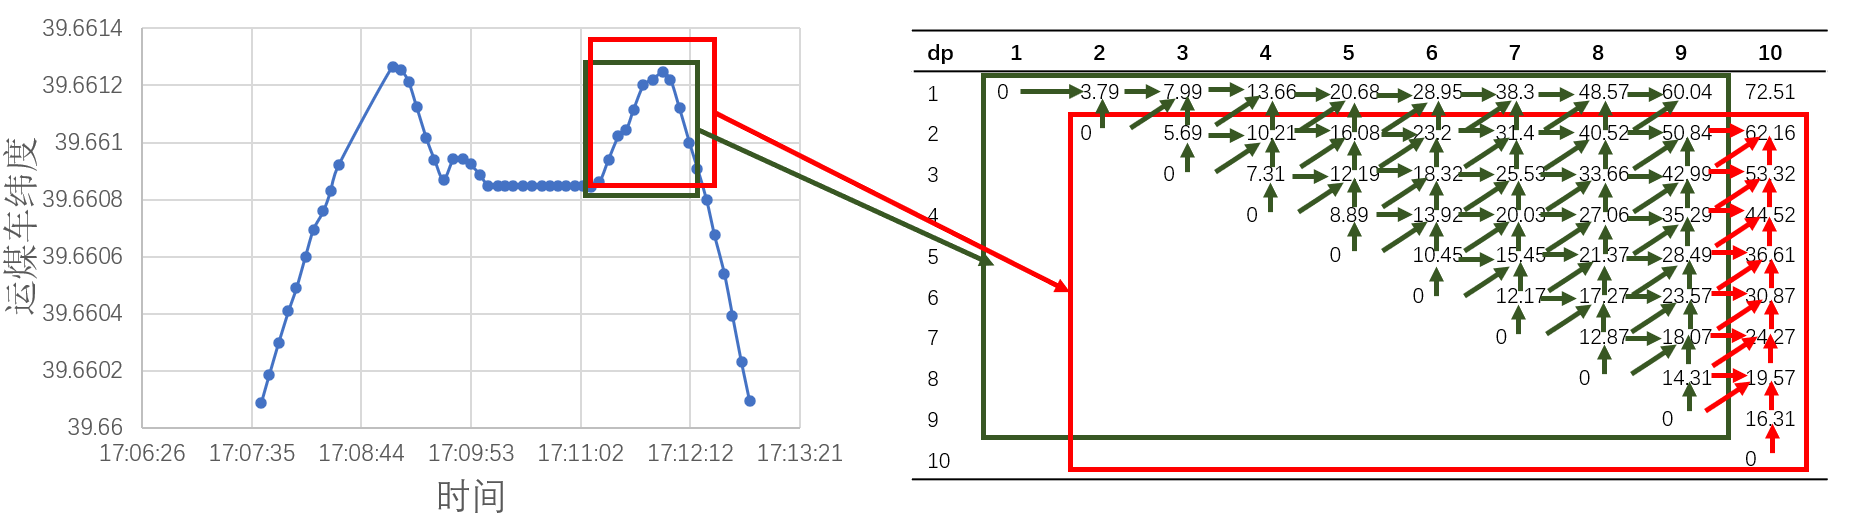
\includegraphics[width=0.86\linewidth]{latitude_stream_matrix.png}
  \caption{运煤车纬度变化与对称度状态转移过程}
  \label{fig:latitude_stream_matrix}
\end{figure}

\subsection{流式对称模式挖掘算法}
本节根据上述对称模式挖掘方法在流式数据上的分析和扩展,
提出了相应的流式挖掘算法。在流式应用场景中,
触发计算的是新数据点的到达,其他位于窗口内的数据点已经到达
并保存,无需重复输入。因此,需要自定义并维护一个双端队列,
只保存与新数据点位于同一个窗口$w$内的数据点,作为流式计算的
状态信息。并且,由图~\ref{fig:latitude_stream_matrix}的
状态转移矩阵可以发现,对称模式流式挖掘算法模型并不需要保存
完整的对称度矩阵,当新增一个数据点$p_t$时,只需要用到
对称度矩阵的最后一列状态来推导和$p_t$相关的状态,从而优化
空间复杂度。总之,对称模式流式挖掘算法只需要长度约束$w$和
新增数据点$p_t$作为输入,此外,由于流式数据是动态、源源不断
到来的,模式识别需要实时报警,且允许出现存在重叠的对称模式。
因此,之前计算对称模式第二类阈值的方法不再适用,只使用第一类
阈值过滤对称模式。算法4.1展示了时间序列对称模式流式挖掘算法
的计算流程,第1-4行对流式框架所需的时间序列$X$和对称度阈值$d$,
第5-12行进行冷启动处理,当数据点数小于$w$时更新对称度状态$dp$
并统一判断为非对称模式。第13-17行倒序计算流式时间序列的对称性,
以保证下次处理时$X$也只有$w$个数据点,
第18行将时间序列$X$中第一个数据点删除,第19-23行
对数据点数大于$w$的时间序列计算对称度状态,
并通过比较是否超过对称度阈值,判断是否为对称模式。
该算法的时间和空间复杂度
均为$O\left(w\right)$,具有较高的时间效率和较快的响应速度。

\renewcommand{\algorithmicrequire}{\textbf{输入:}\unskip}
\renewcommand{\algorithmicensure}{\textbf{输出:}\unskip}

\begin{algorithm}
  \caption{时间序列对称模式流式挖掘算法$calculate\_streaming\_symmtric\_pattern$}
  \label{alg:streaming_symmetric_pattern}
  \small
  \begin{algorithmic}
    \REQUIRE 新数据点$p_t$,长度约束$w$
    \ENSURE 布尔型变量,标志$S=\left(p_{t-w+1},p_{t-w+2},…,p_t \right)$是否为对称子序列

    \STATE 将$p_t$置于时间序列$X$中
    \IF{$t > 1$}
      \STATE $d=d+D\left(p_{t}, p_{t-1}\right)$
    \ENDIF

    \IF{$t < w$}
      \STATE $i \leftarrow t-1$
      \WHILE{$i > 1$}
        \STATE $dp_{i,t} \leftarrow D\left(p_{i}, p_{t} \right) + \min \left(dp_{i,t-1},dp_{i+1,t},dp_{i+1,t-1}\right)$
        \STATE $i \leftarrow i-1$
      \ENDWHILE
      \RETURN false
    \ENDIF

    \STATE $i \leftarrow t-1$
    \WHILE{$i > t-w+1$}
      \STATE $dp_{i,t} \leftarrow D\left(p_{i}, p_{t} \right) + \min \left(dp_{i,t-1},dp_{i+1,t},dp_{i+1,t-1}\right)$
      \STATE $i \leftarrow i-1$
    \ENDWHILE

    \STATE 将$p_(t-w+1)$时间序列X中删除;
    \IF{$dp_{t-w+1,t}/t > d/(n-1)$}
      \RETURN false
    \ELSE
      \RETURN true
    \ENDIF
  \end{algorithmic}
\end{algorithm}

\section{自适应窗口的设计与实现}
时间序列的数据和模式均具有很强的随机性,同一个时间序列中的
对称模式其数据点个数可能不严格相等,而是处于某个合理范围之内。
以挖掘机为例,挖掘不同的坑道时,斗杆移动的轨迹就不同。
当对称模式长度约束设置得较大时,长度较小的模式则挖掘不出。
而当人为设置长度约束为所有对称模式的最小长度时,
尽管可以保证挖掘出长度较小的对称模式,
但是较长模式的信息却经常存在缺失,影响算法挖掘结果的完整性。
图~\ref{fig:excavator_diff_route}展示了挖掘机在不同坑道
挖掘作业斗杆外摆工况变化时间序列。若设定对称子序列的数据点个数
即窗口长度为坑道a的序列长度,则坑道b的对称子序列不能完全挖掘。
因此,当需要挖掘的
对称模式长度不一时,窗口需要在原始长度约束大小上进行自适应的变化
以挖掘出完整的对称模式。本节利用数据点差分的分布特征,
设计了一种自动调节大小的窗口算法。

根据时间序列对称性的定义,在设定对称子序列的长度$w$之后,
挖掘出的对称时间子序列$X=\left(p_{i},p_{i+2},…,p_{i+w-1} \right)$
的首尾点$p_{i}$和$p_{i+w-1}$必定匹配。
换言之,首尾点的距离若接近0,
则证明该窗口大小合适;若远大于0,则证明需调大窗口,
以完整获取对称子序列的全部信息。
因此,可以使用时间子序列首尾点的距离来衡量窗口大小设置得
是否合适。
\begin{figure}
  \centering
  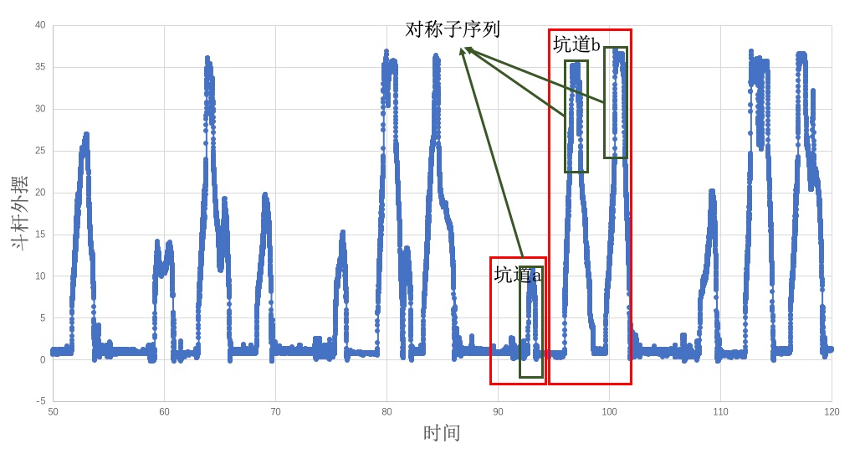
\includegraphics[width=0.86\linewidth]{excavator_diff_route.png}
  \caption{挖掘机在不同坑道挖掘作业斗杆外摆工况时间序列}
  \label{fig:excavator_diff_route}
\end{figure}

然而,真实工业场景中的匹配数据点往往具有误差,
并不一定满足首尾点距离为0。因此,本文考虑利用相邻点距离
所组成数据集的分布特点,判断窗口是否应当扩张。
根据工业大数据时间序列点的随机性,首尾数据点的距离所组成的
数据集应满足正态分布的特点[13],且其均值为0。也就是说,
若一个窗口内的相邻点距离集合为
$s=\left\{D\left(p_{1}, p_{2}\right), D\left(p_{2}, p_{3}\right), \ldots, D\left(p_{n-1}, p_{n}\right)\right\}$,
则首尾数据点距离的应满足均值为$\mu=0$且标准差$\sigma=\sigma_s$
的正态分布。按照3$\sigma$原则,首尾数据点的距离应在
$\left[0,3\sigma\right]$范围之内。

此外,考虑到相邻点的距离属于差分计算。
因此,相比标准差,绝对中位差更加适合度量
相邻点距离集合的分布差异。
绝对中位差指的是所有元素与其中位数的偏差的绝对值,
相比标准差具有更强的鲁棒性,
且已有较为成熟的近似算法加快计算[14]。因此,本节使用窗口内
相邻数据点的距离绝对中位差作为$\sigma$,
首尾点的距离应在$\left[0,3\sigma\right]$之间。
指定窗口的基础长度约束$w_{base}$和最长长度约束$w_{max}$,
若窗口的终点和起点的距离
在$\left[0,3\sigma\right]$范围之内,则窗口闭合。
否则,则继续调大窗口,直到窗口大小为$w_{max}$为止。
具体的计算流程如算法~\ref{alg:adaptive_window}所示。

\renewcommand{\algorithmicrequire}{\textbf{输入:}\unskip}
\renewcommand{\algorithmicensure}{\textbf{输出:}\unskip}

\begin{algorithm}[h]
  \caption{自适应窗口算法$adaptive\_window$}
  \label{alg:adaptive_window}
  \small
  \begin{algorithmic}
    \REQUIRE 时间序列$X=\left(p_1,p_2,…,p_n\right)$,基础模式长度$w_{base}$,最长模式长度$w_{max}$
    \ENSURE 调整后的窗口大小$t$

    \STATE $\sigma=\operatorname{mad}(X, w_{max})$
    \STATE $t \leftarrow w_{base}$
    \STATE $i \leftarrow 1$
    \WHILE{$i+t<|X| \& \& t<w_{max} \& \& D\left(p_{i}, p_{i+1}\right)>3 \sigma$}
      \STATE $t \leftarrow t+1$
    \ENDWHILE
    \RETURN $t$
  \end{algorithmic}
\end{algorithm}

\section{本章小结}
本章主要介绍了时间序列对称模式挖掘在更多应用场景下的扩展。
首先,流式时间序列数据作为一种在工业和金融领域经常出现的数据
类型,对其进行对称模式挖掘具有重要的研究价值。但是,
度量所有时间子序列的对称性会产生大量重复计算,时间效率低,
且对称度阈值也不好判定。本章根据全局时间序列对称模式挖掘算法
的状态推导方式,在对称度矩阵上创造性地引入了滑动窗口,
在不违反对称度状态连续性和单调性的前提下,采用以空间换时间的
策略将流式对称模式的计算时间复杂度由$O\left(w^2\right)$
提升至了$O\left(w\right)$。
此外,为了在时间序列中挖掘完整的对称模式,本章还在对称模式的
挖掘过程中引入了自适应窗口,通过时间序列的数据特征自动地调节
窗口大小,以保证挖掘对称模式的完整性。对称模式挖掘在不同的
应用中具有很好的可扩展性,通过设置不同的约束可以灵活地调整
对称模式挖掘算法,从而满足不同场景的需要。

% 模板支持 BibTeX 和 BibLaTeX 两种方式处理参考文献。
% 下文主要介绍 BibTeX 配合 \pkg{natbib} 宏包的主要使用方法。


% \section{顺序编码制}

% 在顺序编码制下,默认的 \cs{cite} 命令同 \cs{citep} 一样,序号置于方括号中,
% 引文页码会放在括号外。
% 统一处引用的连续序号会自动用短横线连接。

% \thusetup{
%   cite-style = super,
% }
% \begin{tabular}{l@{\quad$\Rightarrow$\quad}l}
%   \verb|\cite{zhangkun1994}|               & \cite{zhangkun1994}               \\
%   \verb|\citet{zhangkun1994}|              & \citet{zhangkun1994}              \\
%   \verb|\citep{zhangkun1994}|              & \citep{zhangkun1994}              \\
%   \verb|\cite[42]{zhangkun1994}|           & \cite[42]{zhangkun1994}           \\
%   \verb|\cite{zhangkun1994,zhukezhen1973}| & \cite{zhangkun1994,zhukezhen1973} \\
% \end{tabular}


% 也可以取消上标格式,将数字序号作为文字的一部分。
% 建议全文统一使用相同的格式。

% \thusetup{
%   cite-style = inline,
% }
% \begin{tabular}{l@{\quad$\Rightarrow$\quad}l}
%   \verb|\cite{zhangkun1994}|               & \cite{zhangkun1994}               \\
%   \verb|\citet{zhangkun1994}|              & \citet{zhangkun1994}              \\
%   \verb|\citep{zhangkun1994}|              & \citep{zhangkun1994}              \\
%   \verb|\cite[42]{zhangkun1994}|           & \cite[42]{zhangkun1994}           \\
%   \verb|\cite{zhangkun1994,zhukezhen1973}| & \cite{zhangkun1994,zhukezhen1973} \\
% \end{tabular}



% \section{著者-出版年制}

% 著者-出版年制下的 \cs{cite} 跟 \cs{citet} 一样。

% \thusetup{
%   cite-style = author-year,
% }
% \begin{tabular}{l@{\space$\Rightarrow$\space}l}
%   \verb|\cite{zhangkun1994}|                & \cite{zhangkun1994}                \\
%   \verb|\citet{zhangkun1994}|               & \citet{zhangkun1994}               \\
%   \verb|\citep{zhangkun1994}|               & \citep{zhangkun1994}               \\
%   \verb|\cite[42]{zhangkun1994}|            & \cite[42]{zhangkun1994}            \\
%   \verb|\citep{zhangkun1994,zhukezhen1973}| & \citep{zhangkun1994,zhukezhen1973} \\
% \end{tabular}

% \vskip 2ex
% \thusetup{
%   cite-style = super,
% }
% 注意,引文参考文献的每条都要在正文中标注
% \cite{zhangkun1994,zhukezhen1973,dupont1974bone,zhengkaiqing1987,%
%   jiangxizhou1980,jianduju1994,merkt1995rotational,mellinger1996laser,%
%   bixon1996dynamics,mahui1995,carlson1981two,taylor1983scanning,%
%   taylor1981study,shimizu1983laser,atkinson1982experimental,%
%   kusch1975perturbations,guangxi1993,huosini1989guwu,wangfuzhi1865songlun,%
%   zhaoyaodong1998xinshidai,biaozhunhua2002tushu,chubanzhuanye2004,%
%   who1970factors,peebles2001probability,baishunong1998zhiwu,%
%   weinstein1974pathogenic,hanjiren1985lun,dizhi1936dizhi,%
%   tushuguan1957tushuguanxue,aaas1883science,fugang2000fengsha,%
%   xiaoyu2001chubanye,oclc2000about,scitor2000project%
% }。

% !TeX root = ../thuthesis-example.tex

\chapter{实验与结果分析}
本节将会对第3章和第4章提出的时间序列对称模式挖掘算法进行
实验验证和结果分析工作。
具体而言,主要包括对第3章节提出的全局对称模式挖掘算法
进行结果对比和验证,对分段对称模式挖掘算法进行效果和性能评估。
并且,通过调节对称模式长度约束验证自适应窗口对模式挖掘完整性的提升。

\section{实验环境}
本文试验所使用的环境如表~\ref{tab:experiment_enviroment}所示。
实验所使用的数据集,一方面来自UCR提供的时间序列数据集,
另一方面来自真实应用场景的时间序列数据。
UCR中每类数据集重的时间序列长度都相同。
真实的数据集来自传感器采集的工业大数据,
其中每条时间序列都包含多个工况信息,且都未进行标准化,
对称模式挖掘有一定难度。
为了方便在同一量纲下使用对称模式挖掘算法进行计算,
实验所用所有数据集均经过了标准化操作。
针对不同实验对于数据的要求,
本文选择合适的数据集进行实验,具体的数据集信息将在实验过程中
进行详述。

\begin{table}
  \centering
  \caption{实验环境介绍}
  \begin{tabular}{ll}
    \toprule
    实验环境     & 具体参数                          \\
    \midrule
    操作系统     & macOS 版本 10.15.5                \\
    处理器       & 2.4 GHz 四核Intel Core i5         \\
    内存         & 16 GB 2133 MHz LPDDR3             \\
    固态硬盘     & 256GB                             \\
    代码语言     & Python                            \\
    集成开发环境 & PyCharm 2020.1(Community Edition) \\
    \bottomrule
  \end{tabular}
  \label{tab:experiment_enviroment}
\end{table}

\section{全局对称模式挖掘效果评估实验}
由于时间序列的数据值是连续数据,
具有一定的随机性和波动性,不同于对称字符串,
现有研究中并不存在一个明确统一的对称性度量算法。
因此,本文基于全局时间序列的数据特征,提出了一种
基于区间动态规划和全局匹配的对称性度量算法。
为了检测对称性度量算法的效果,
本文在UCR数据集中选择了两个具有明显全局对称性的时间序列数据集
和两个不具有全局对称性的时间序列数据集,
这4个数据集的详细介绍如表~\ref{tab:experiment_dataset}所示。

在这4个数据集中,GunPointAgeSpan的时序数据表示
一套完整的持枪动作,而UMD的时间序列表示的是实验室信号合成数据,
两者都具有对称的物理意义。而GestureMidAirD1和MixedShapes
分别是手势轨迹和由普通二维形状转换而来的时间序列数据,
不具有对称性。分别对这两组包含正负样本的数据集进行实验,
可以验证本文全局对称性度量算法的有效性。为保证正负样本的数据
条数大致相同,不会出现数据倾斜问题,本文通过采样保证了
对称数据集和非对称数据集的时间序列条数均为147。

\begin{table}
  \centering
  \caption{实验数据集介绍}
  \begin{tabular}{ccccc}
    \toprule
    数据集名称      & 来源         & 类型 & 数据条数 & 长度 \\
    \midrule
    GestureMidAirD1 & 3D手势轨迹   & 运动 & 47       & 361  \\
    GunPointAgeSpan & 完整举枪动作 & 运动 & 135      & 150  \\
    MixedShapes     & 二维形状转换 & 图像 & 100      & 1024 \\
    UMD             & 信号合成     & 模拟 & 12       & 150  \\
    \bottomrule
  \end{tabular}
  \label{tab:experiment_dataset}
\end{table}

本文为全局时间序列对称性度量算法设置了两个算法作为对照组实验,
其一为利用原始和反转时间序列相似性度量对称性的方法,
另一个是通过对称中心两侧子序列的相似性度量对称性的方法。
由于时间序列数据的连续性和不稳定性,不同类型时间序列数据的对称中心
不确定,因此,本文选用时间序列的几何中心作为其对称中心。
此外,正如2.4节所述,时间序列相似性度量算法种类多样,
仅基于形状的相似性度量方法就远不止一种。本文选择了包括基于
曼哈顿距离、欧式距离、DTW距离和FastDTW距离在内的4种相似性
度量方法,其中每种方法都可以用来为对照组的两个算法提供相似性度量
计算。表~\ref{tab:experiment_algorithm}对本实验涉及到的9种时间序列
对称性度量算法进行了介绍。
由于不同度量方法的计算方式不同,不同数据集的时间序列长度
也不同,为了在同一量纲上进行比较,在通过全局对称性度量算法和
其他相似性度量算法得到时间序列的全局对称度之后,需要再计算其
与时间序列长度的比值得到单点对称度,作为最终统一衡量时间序列
对称性的值。
\begin{table}
  \centering
  \caption{实验算法介绍}
  \begin{tabular}{ll}
    \toprule
    算法名称          & 计算方式                            \\
    \midrule
    symmetry          & 基于全局时间序列对称性度量算法      \\
    manhattan         & 基于原始和反转时间序列的曼哈顿距离  \\
    euclidean         & 基于原始和反转时间序列的欧式距离    \\
    dtw               & 基于原始和反转时间序列的DTW距离     \\
    fastdtw           & 基于原始和反转时间序列的FastDTW距离 \\
    center\_manhattan & 基于中心点两侧时间序列的曼哈顿距离  \\
    center\_euclidean & 基于中心点两侧时间序列的欧式距离    \\
    center\_dtw       & 基于中心点两侧时间序列的DTW距离     \\
    center\_fastdtw   & 基于中心点两侧时间序列的FastDTW距离 \\
    \bottomrule
  \end{tabular}
  \label{tab:experiment_algorithm}
\end{table}

首先在对称数据集上进行对称模式挖掘实验,分析不同数据集
时间序列的对称度结果,以及对称度阈值对对称模式挖掘的影响。
图~\ref{fig:symmetry_compare}展示了在两个对称数据集上,
不同对称性度量算法计算得到的对称度结果。经过对比可以发现,
本文所提出的全局时间序列对称性度量算法(symmetry算法)
计算得到的对称度总是最小的,
不仅小于基于原始和反转时间序列的相似性度量对称性的算法,
也小于基于中心点两侧时间序列相似性度量对称性的算法。
对于相同的对称度阈值,本算法可以挖掘出数量尽可能多的
对称时间序列和对称模式。除此之外,从本结果中还可以看出,
尽管GunPointAgeSpan和UMD数据集的时间序列具有物理意义上
的对称性,而且时间序列的长度相同,甚至都经过了标准化处理,
但其对称度的分布范围仍然相差甚大。以symmetry算法为例,在
GunPointAgeSpan数据集上度量135条时间序列得到的平均对称度
是0.026,而在UMD数据集上度量12条时间序列得到的平均对称度
仅为0.013,不同来源的数据集因为数据特征的差别其对称度阈值
差距较大,这为对称模式的挖掘也带来了困难,
从侧面证明了本文提出的对称度阈值算法的重要性。
\begin{figure}
  \centering
  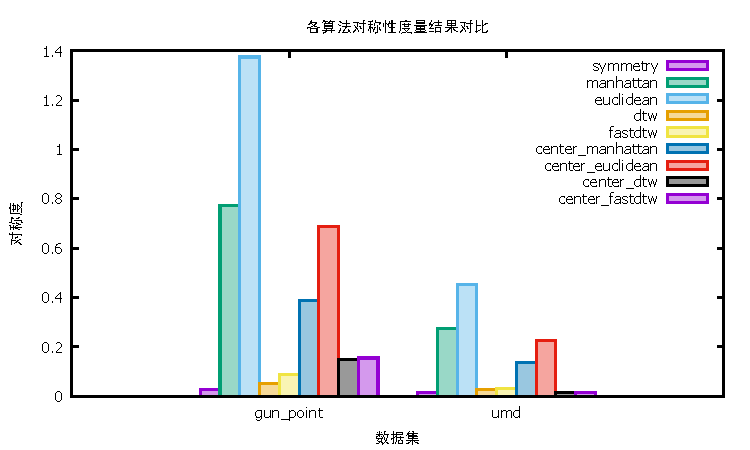
\includegraphics[width=0.86\linewidth]{symmetry.pdf}
  \caption{对称数据集不同算法的对称性度量结果}
  \label{fig:symmetry_compare}
\end{figure}

在真实的工业领域,往往采用领域专家指定对称度阈值的方式过滤对称模式。
因此,本文在GunPointAgeSpan和UMD这两个具有全局对称性的数据集上进行实验,
在计算得到数据集中时间序列的对称度之后,通过调整对称度阈值,
分析对称模式的挖掘效果。为保证在GunPointAgeSpan和UMD数据集
分别选择合适的对称度阈值变化范围
,本文通过统计每个数据集上所有时间序列
相邻点距离的最小值和最大值作为对称度阈值的变化范围。
图~\ref{fig:symmetry_heatmap}展示了当对称度阈值
发生变化时,对称模式挖掘效果随之发生的变化。其中,
使用对称中心度量对称性的算法用前缀c加以区分。
从图中可以看出两点:
\begin{enumerate}
  \item 尽管同为对称数据集,不同来源的时间序列变化
        剧烈程度不同,数据的差异程度也不同。
        即使经过标准化也不能完全消弭这种差异。
        经过标准化的Gun数据集相邻点之间的距离最大可达1.76,
        而UMD数据集相邻点之间的距离最大仅为0.7,
        不利于领域专家人为确定对称度阈值。结合图~\ref{fig:symmetry_compare}
        关于Gun和UMD数据集对称度度量结果的比较,发现时间序列相邻点变化剧烈的
        数据集,其对称度也偏大,对称度和时间序列相邻点距离呈正相关。
        因此,基于时间序列
        数据特征确定对称度阈值的算法是可行的。
  \item 随着对称度阈值的增大,全局对称模式挖掘算法很快收敛,能挖掘出
        对称数据集Gun和UMD中所有的对称模式。
        同样,基于DTW距离和FastDTW距离的
        对称性度量方法也很快收敛。
        但是,基于欧氏距离和曼哈顿距离的算法却需要较高
        的对称度阈值才能挖掘出数据集中所有的对称模式。
        甚至在Gun数据集中,eculidean算法在
        对称度阈值达到上限1.8时仍然只能挖掘出低于60\%的对称模式。
        证明了相比一一对应,基于全局匹配
        的对称性度量算法在对称模式挖掘具有更好的稳定性。

\end{enumerate}
\begin{figure}
  \centering
  \subcaptionbox{GunPointAgeSpan\label{fig:gun_heatmap}}
  {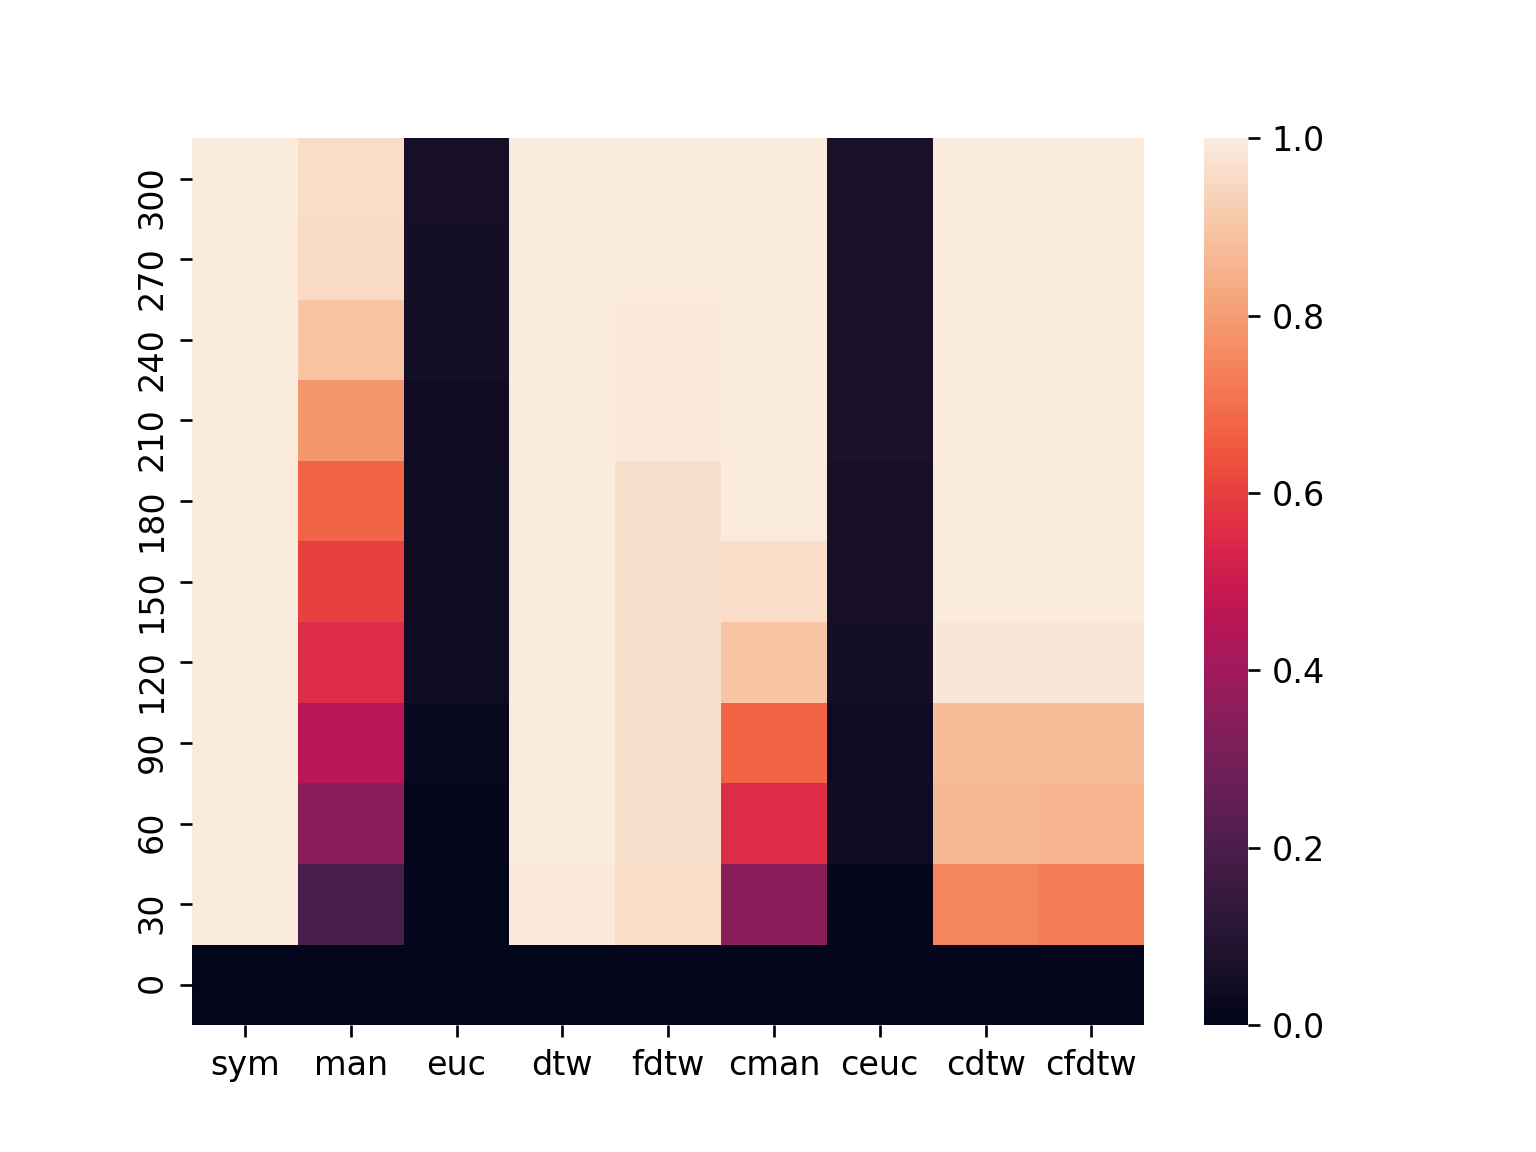
\includegraphics[width=0.43\linewidth]{gun_heatmap.png}}
  \subcaptionbox{UMD\label{fig:umd_heatmap}}
  {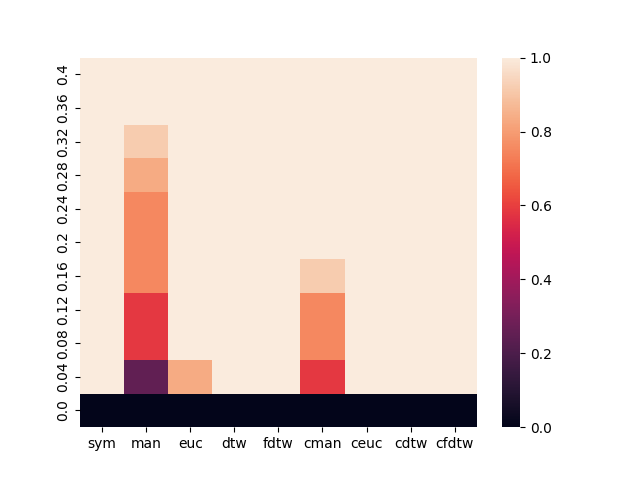
\includegraphics[width=0.43\linewidth]{umd_heatmap.png}}
  \caption{对称模式挖掘效果随对称度阈值变化}
  \label{fig:symmetry_heatmap}
\end{figure}

由于不同来源的时间序列数据特征差别很大,
采用领域专家直接指定对称度阈值的方式在处理多源数据集时并不现实。
本文使用相邻点之间的距离作为匹配点之间
的距离阈值参考,进而得到全局时间序列的对称度阈值,以进行全局对称模式的
挖掘。接下来本文将对表~\ref{tab:experiment_dataset}中所示
的4个数据集进行全局对称模式挖掘算法的效果实验,并以准确率,精确率,
召回率和F值作为效果的评价指标。在这4个数据集中,GunPointAgeSpan和UMD数据集
具有对称性,而MixedShapes和GestureMidAirD1数据集没有对称性。
在实验过程中,本文把对称模式标记为正类(positive),把非对称模式标为负类(negative)。
当算法在对称数据集中发现对称模式时,这类时间序列用TP表示。当算法
在对称数据集中发现非对称模式时,这类时间序列用FN表示。当算法
在非对称数据集中发现对称模式时,这类时间序列用FP表示。当算法
在非对称数据集中发现非对称模式时,这类时间序列用TN表示。
基于以上四类情况,可以定义时间序列对称模式挖掘算法的
准确率(Accuracy),精确率(Precision)和召回率(Recall)和F值。
其中,准确率表示挖掘正确的样本数和总样本数的比值。
准确率是最为常见的一类效果统计指标。
式~\ref{eq:precision}表示了精确率的计算方式。
精确率又叫查准率,定义为在所有被预测为正的样本中,
实际为正样本的概率,在本实验中的含义是预测为对称模式的时间序列中有多少是真正的对称时间序列,
式~\ref{eq:precision}表示了精确率的计算方式。召回率又叫查全率,定义为在所有真实为正
的样本中,预测为正样本的概率,在本实验中的含义是
真实为对称模式的时间序列中有多少被预测为了对称时间序列。
式~\ref{eq:recall}表示了召回率的计算方式。F值的定义是准确率和召回率的加权平均数,
为平衡准确率和召回率,本文选择F1值作为F值度量结果,式~\ref{eq:f1}表示了
F1值的计算方式。
\begin{equation}
  Accuracy=\frac{TP+TN}{TP+FP+TP+TN}
  \label{eq:Accuracy}
\end{equation}
\begin{equation}
  Precision=\frac{TP}{TP+FP}
  \label{eq:precision}
\end{equation}
\begin{equation}
  Recall=\frac{TP}{TP+FN}
  \label{eq:recall}
\end{equation}
\begin{equation}
  F1=\frac{2 \times Precision \times Recall}{Precision+Recall}
  \label{eq:f1}
\end{equation}

准确率十分直观地展示了不同算法模式挖掘的效果。
图~\ref{fig:accuracy_compare}即为不同算法挖掘对称模式
准确率的对比结果。从图中可以很明显的看出,
symmetry算法挖掘对称模式的准确率远高于其他算法。
即便是同样采用全局匹配的基于DTW和FastDTW距离的对称模式挖掘算法,
其准确率也低于symmetry算法。
除此之外,从图中还可以对比得到,算法的对称模式挖掘效果与
对称中心的明确与否关系不大,而与对称模式的具体匹配方式关系很大。
同为基于DTW距离的挖掘算法,采用对称中心两侧子序列与采用
原始和反转时间序列的相似性度量对称性的方式,其效果十分相近。
而基于DTW距离和基于曼哈顿距离的算法挖掘效果却相差很大。
基于曼哈顿距离和欧氏距离的对称模式挖掘算法几乎只能识别对一半
的模式,在实验数据集样本均衡的前提下,其准确率与随机猜测已差别不大,
几乎不具有实用价值。这证明基于时间扭曲的全局匹配方式要远优于一一对应
的匹配方式。
\begin{figure}
  \centering
  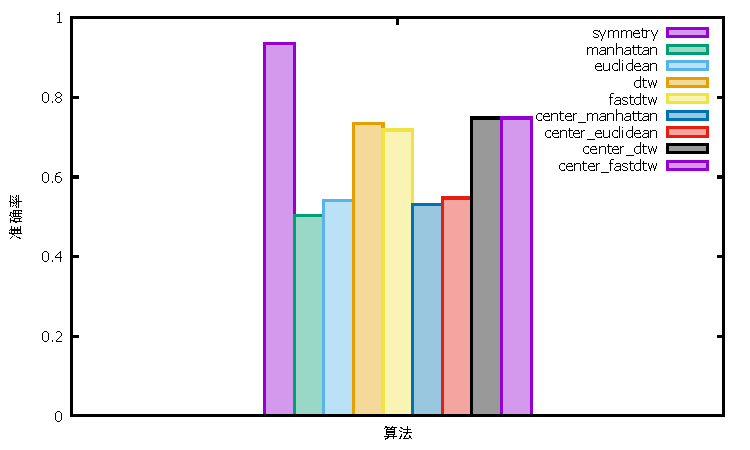
\includegraphics[width=0.86\linewidth]{accuracy.pdf}
  \caption{不同对称模式挖掘算法的准确率度量结果}
  \label{fig:accuracy_compare}
\end{figure}

尽管准确率十分直观地度量了时间序列对称模式挖掘的效果,
但由于其过于简单,易受到实验数据集的影响。
为了综合评价算法的挖掘效果,本文选用F值表示算法的对称模式挖掘效果。
因为精确率是挖掘出的对称模式中真正对称模式所占的比例,表示了
算法挖掘对称模式的准确程度。而召回率是对称数据集中挖掘出对称模式
所占的比例,衡量了算法对于对称模式的识别能力,召回率越高,表明算法
能挖掘出更全面的对称模式。很明显,精确率和召回率是两个
冲突的指标。精确率是关于算法挖掘准确的度量,召回率是关于算法挖掘覆盖面的
度量。一个优秀的算法应该同时具有较高的精确率和召回率。
F值就是用来综合评估算法的精确率和召回率。在实验中,本文采用F1值度量
模型效果的优劣。图~\ref{fig:fscore_compare}展示了在表~\ref{tab:experiment_dataset}
所示的数据集下进行对称模式挖掘,不同F值的结果。从图中可以发现,symmetry
算法的F值要远高于其他算法,证明了全局对称模式挖掘算法的有效性。
\begin{figure}
  \centering
  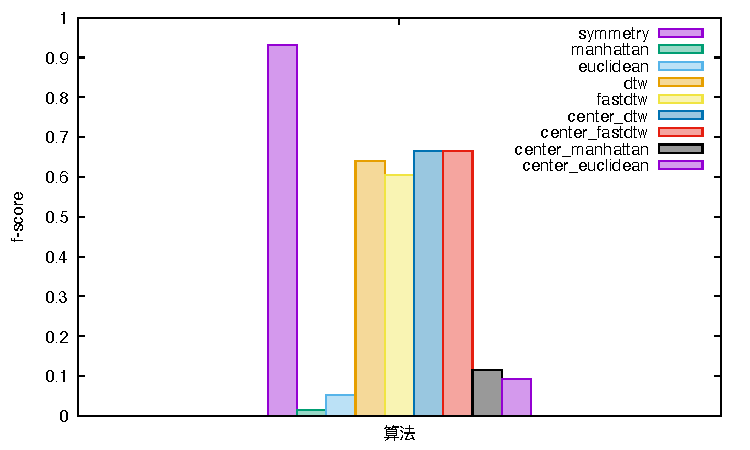
\includegraphics[width=0.86\linewidth]{f-score.pdf}
  \caption{不同对称模式挖掘算法的F-Score度量结果}
  \label{fig:fscore_compare}
\end{figure}

为了更细致的分析不同算法F值差别的原因,表~\ref{tab:experiment_global_algo}
列出了实验对比所有算法的精确率,召回率和F值。观察表格发现,
symmetry算法的召回率非常高,几乎是基于DTW距离的对称性度量算法
的两倍,证明了symmetry算法在不同数据集上挖掘对称模式的全面性,
能挖掘出尽可能多的对称模式。
而基于欧氏距离和曼哈顿距离的对称性度量算法,由于采取一一对应
的匹配方式,忽略了时间序列在不同阶段的采样率和持续时间不同,
其召回率非常低。
除此之外,全局对称模式挖掘算法采用基于时间序列数据特征的相邻点距离均指
作为对称度阈值。由于算法能为不同来源的数据集确定合适的对称度阈值,
因此所有对称模式挖掘算法的精确率都非常高,
在实验提供的数据集上没有出现挖掘出错误对称模式的情况。


\begin{table}
  \centering
  \caption{不同算法对称模式挖掘效果评估}
  \begin{tabular}{llll}
    \toprule
    算法              & Precision & Recall & F-score \\
    \midrule
    symmetry          & 1.0       & 0.871  & 0.931   \\
    manhattan         & 1.0       & 0.007  & 0.014   \\
    euclidean         & 1.0       & 0.027  & 0.053   \\
    dtw               & 1.0       & 0.469  & 0.639   \\
    fastdtw           & 1.0       & 0.435  & 0.606   \\
    center\_manhattan & 1.0       & 0.061  & 0.115   \\
    center\_euclidean & 1.0       & 0.048  & 0.092   \\
    center\_dtw       & 1.0       & 0.497  & 0.664   \\
    center\_fastdtw   & 1.0       & 0.497  & 0.664   \\
    \bottomrule
  \end{tabular}
  \label{tab:experiment_global_algo}
\end{table}

\section{分段对称模式效果评估实验}
3.3.2节对全局对称模式挖掘算法进行了效果评估实验。除了具有
全局对称性的时间序列,更多的对称模式以子模式的方式嵌入在
长时间序列之中。需要采用分段对称模式挖掘算法对其进行挖掘。
本文采用1个人工数据集和3个真实数据集进行实验。具体的数据信息
如表~\ref{tab:segment_dataset}中所示。
其中,人工数据集包含30000个数据点,
除部分噪声影响之外,原始数据为以360个点为一个完整周期的
正弦函数采样数据。真实数据集1为GPS轨迹数据,共33500个数据点,
主要采集了运输车运输货物5天内的行驶轨迹结合实际情况以及
数据采集信息。其运输过程为在固定起点和终点之间运送煤炭,每一趟
GPS轨迹信息具有物理上的对称性。但是,
由于车速和运输路线的不同,运输车运输一趟的
平均时间为30分钟,最长为48分钟,时间序列的长度并不固定。
真实数据集2为等时间间隔采样的挖掘机挖斗数据,
共35189个数据点,主要采集了挖掘机在挖掘过程中各个工况的变化。
挖掘机每次作业形成的工况时间序列具有对称性。
然而,由于挖掘机每次挖掘的坑道不一致,且两次作业间存在等待期,
导致挖掘机工况对称模式持续的时间长度变化较大。
真实数据集3为上证指数2016年至2019年以天为单位变化
的时间序列,共有3186个数据点。
由于股票数据具有长期增长的趋势性特征,其对称模式出现较少,
可通过人工标注对称模式作为正确结果。
实验采用的4个数据集各有特点:
人工数据集具有明显的周期性;运输车轨迹数据集运行时间较长,
对称性较为明显;挖掘机工况数据集停机时间较长,噪声较多,
对称性不易挖掘;上证指数数据集对称子模式非常少,持续时间同样很长。
若算法在这4类数据集上的表现均比较良好,
则证明了分段对称模式挖掘算法的有效性。

\begin{table}
  \centering
  \caption{分段对称模式时间序列数据集}
  \begin{tabular}{llll}
    \toprule
    数据集名称       & 来源                   & 时间序列长度  \\
    \midrule
    合成数据集       & 正弦函数曲线           & 30000               \\
    GPS轨迹数据集 & 运输车轨迹信息       & 33500              \\
    工况数据集 & 挖掘机作业工况信息 & 35189              \\
    金融数据集       & 上证指数历年变化       & 3186               \\
    \bottomrule
  \end{tabular}
  \label{tab:segment_dataset}
\end{table}

对于总点数和对称模式长度约束不同的时间序列,
需要设定一个评价标准验证分段对称模式挖掘算法的效果。
虽然时间序列模式包含的数据点个数或多或少,
但是给定时间序列中模式的个数通常是固定的。
因此,本文采用对称模式的数量偏差评价真实结果和挖掘结果的相近程度。
式~\ref{eq:variation}展示了偏差率$\delta$的计算方式。
令$r_{truth}$作为时间序列对称模式的真实数量,
$r_{cal}$作为挖掘出的时间序列对称模式的数量。
则用$\delta$评估挖掘结果和真实结果的相似程度,表示挖掘效果
的的误差率。$\delta$越小, 说明挖掘结果越精确。偏差率$\delta$
作为算法的评价指标同样具有应用价值,实际工业场景中常有
统计对称模式数量的需求,例如挖掘机通过一天内的运输趟数记工打卡,
偏差率表示挖掘的运输趟数和真实运输趟数之间的差距,是算法优劣的重要指标。

\begin{equation}
  \delta \left( r_{truth}, r_{cal} \right) = \frac{\left| r_{cal} - r_{truth} \right|}{r_{truth}}
  \label{eq:variation}
\end{equation}

合成数据集,GPS轨迹数据集和工况数据集以秒或者毫秒为单位采集数据,
时间序列长,具有物理意义的对称模式较多,因此,本文在
长度由3000到30000不等的数据量上进行分段对称模式挖掘实验。
而金融数据集以天为单位采集数据,
时间序列长度和对称模式数量均较小,因而
本文在长度由600到3000不等的数据量上对金融数据进行
分段对称模式挖掘实验。
图~\ref{fig:segement_symmetry}展示了在这4个数据集上进行分段对称模式挖掘的效果。
首先是具有严格对称性的合成数据集,由图~\ref{fig:sin_1}和~\ref{fig:sin_2}
可知,除了manhattan算法效果较差之外,其他算法的效果均十分稳定。
分析算法可以得知,当对称模式长度约束设为360时,manhattan算法
以一一对应的方式计算对称度。尽管对称模式只有360个点,但在全部时间序列中
与模式第1个点对应的是下一个模式的第1个点,即第361个点。因此,
manhattan算法会在匹配点计算时产生偏差。
而由于正弦时间序列整体平稳,分段算法确定的对称度阈值也较小,因此其对称模式挖掘效果出现抖动,
当对称度阈值过小时,对称模式无法挖掘。
GPS轨迹没有明确的对称中心,其数据点也由于车辆行驶过程的随机性和采样
传感器的不精确而具有随机误差,同时,对称子模式的长度也不固定。
为保证挖掘效果,本文采用车辆单趟运输轨迹的数据点采样平均值300作为长度约束挖掘对称模式。
由图~\ref{fig:truck_1}和~\ref{fig:truck_2}可知,symmetry算法的偏差率在所有算法中
处于最低水平,表明其挖掘出的对称模式数量和
真实结果最为接近,不仅远超过基于欧氏距离和曼哈顿距离的对称模式挖掘算法,也优于
DTW和FastDTW方法。
在所有方法中,仅有center\_DTW和center\_FastDTW算法和symmetry算法效果较为接近,但也略有不如
。证明分段对称模式挖掘算法具有很高的鲁棒性,在存在误差的数据集中
也能挖掘出正确的对称模式。

图~\ref{fig:excavator_1}和图~\ref{fig:excavator_2}是在挖掘机工况数据集
上进行实验得到的结果。挖掘机一次作业过程的时间序列
具有对称性,但是挖掘机作业过程中间歇阶段较多,作业类型不一致导致对称模式长度不固定,
且伴生着随机的噪音和误差,使得对称模式挖掘任务更为复杂。
尽管如此,symmetry算法仍然将偏差率控制在了0.2以下,且随着
时间序列长度的增加,对称模式挖掘效果逐渐收敛,并无明显下降。
相比之下,基于欧氏距离和曼哈顿距离的对称模式挖掘算法不仅偏差率
较高,而且随时间序列的长度增加,起伏变化不定,稳定性很差。而基于DTW
距离和FastDTW距离的算法其效果也要差于symmetry算法。
金融数据集来源于上证指数10年内的数值变化,金融领域的数据具有很强
的实时性,短期内变化大,对称性不明显。在全局时间序列中,只存在两个局部的
对称子模式。图~\ref{fig:stock_1}和图~\ref{fig:stock_2}展示了
在金融数据集上不同算法挖掘对称模式的偏差率,
从图中可知,基于DTW和FastDTW距离的算法在金融数据集上出现了性能的严重下降,
DTW和FastDTW方法甚至没有挖掘出一个对称模式。相比之下,Symmetry算法的
效果保持稳定,在不同规模的时间序列中均挖掘出了正确数量的对称模式。
此外,center\_euclidean算法挖掘对称模式的效果和Symmetry算法平齐,
分析算法发现,金融数据集单日变化过于剧烈,导致对称度阈值计算结果偏大。
而标准化后的上证指数时间序列欧氏距离相比标准化之前降低明显,
因而center\_euclidean算法的挖掘效果较好。

总之,通过在多源数据集上对不同算法进行对比实验综合发现:
\begin{enumerate}
  \item 从合成数据集、运输车GPS数据集到
  挖掘机工况数据集和金融数据集,对称模式的数量逐渐减少,数据偏差、失配、
  不对齐和噪声干扰逐渐增多,对称模式挖掘的难度不断增大。但是在所有数据集上,
  分段对称模式挖掘算法均有最优的表现。
  \item 同全局对称模式挖掘算法一样,基于一一对应的匹配方式
  在分段对称模式挖掘任务上同样表现较差,远低于基于时间扭曲和全局匹配
  的方法,从而导致对称模式的挖掘效果较差。
\end{enumerate}


\begin{figure}
  \centering
  \subcaptionbox{合成数据集\label{fig:sin_1}}
  {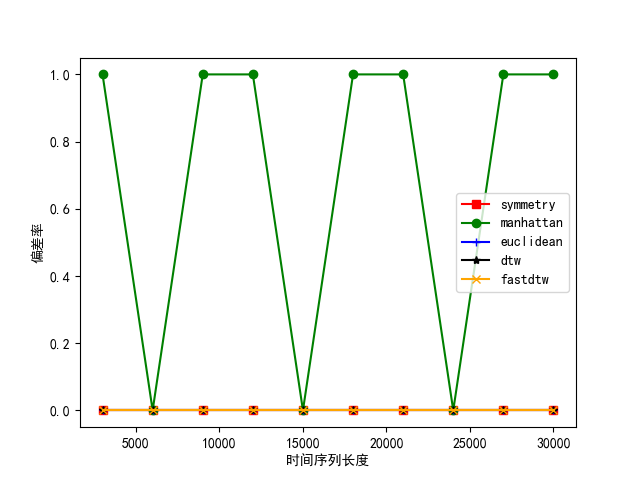
\includegraphics[width=0.43\linewidth]{sin_1.png}}
  \subcaptionbox{合成数据集\label{fig:sin_2}}
  {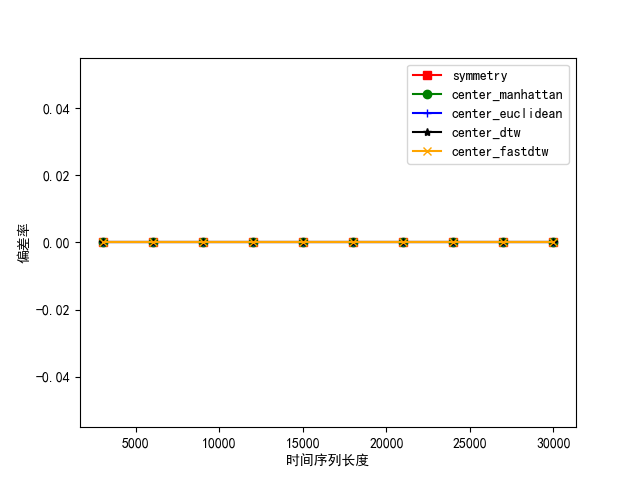
\includegraphics[width=0.43\linewidth]{sin_2.png}}
  \subcaptionbox{GPS轨迹数据集\label{fig:truck_1}}
  {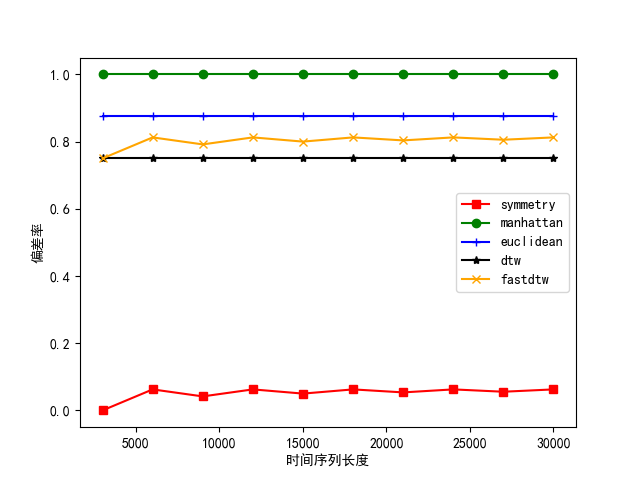
\includegraphics[width=0.43\linewidth]{truck_1.png}}
  \subcaptionbox{GPS轨迹数据集\label{fig:truck_2}}
  {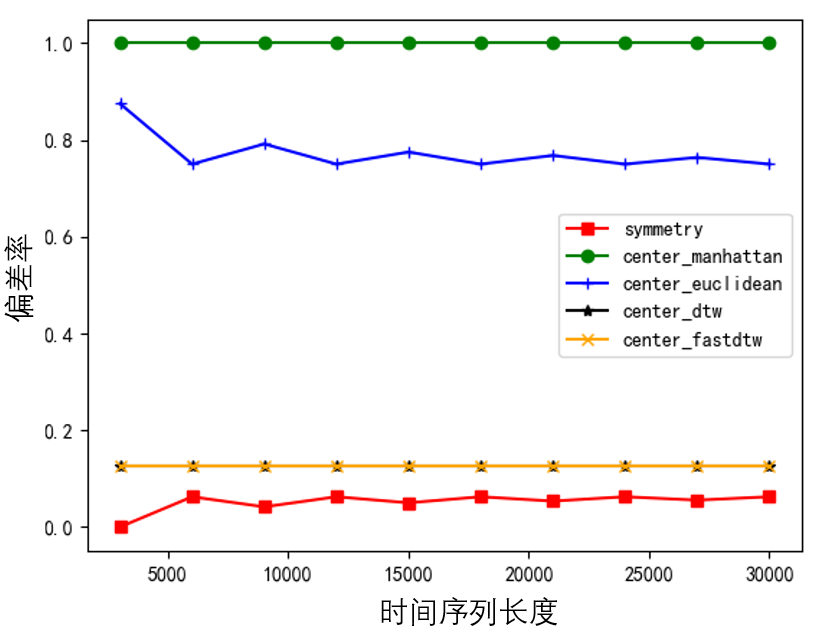
\includegraphics[width=0.43\linewidth]{truck_2.png}}
  \subcaptionbox{工况数据集\label{fig:excavator_1}}
  {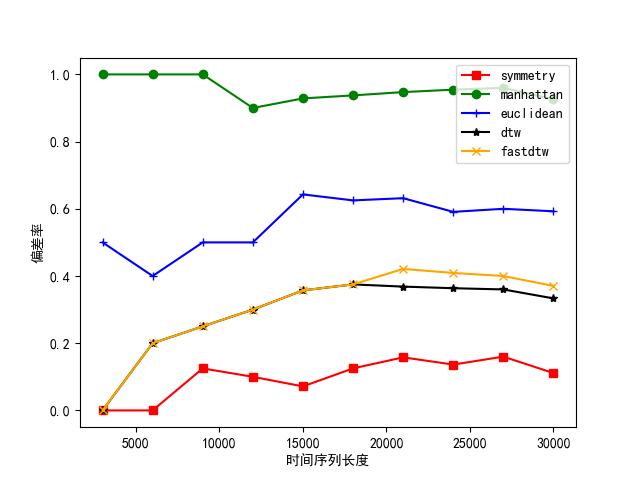
\includegraphics[width=0.43\linewidth]{excavator_1.png}}
  \subcaptionbox{工况数据集\label{fig:excavator_2}}
  {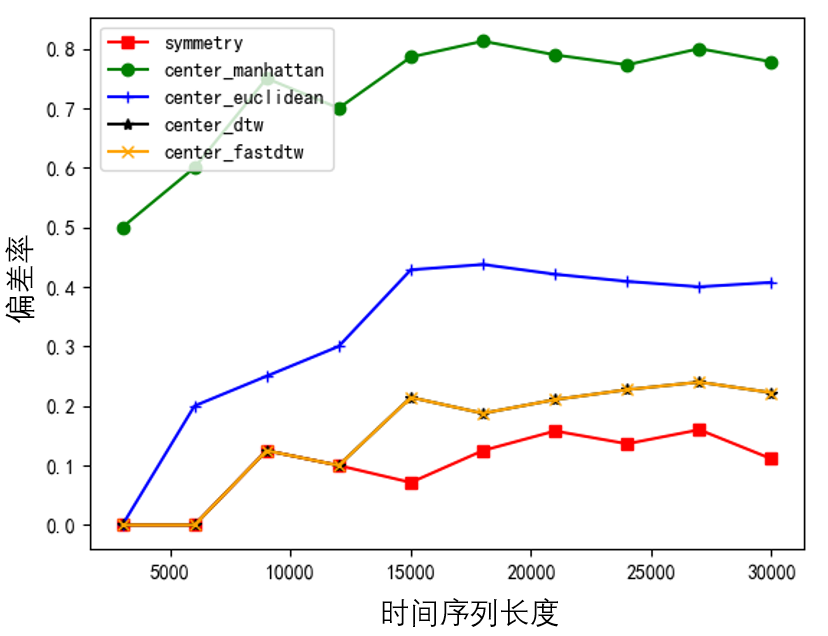
\includegraphics[width=0.43\linewidth]{excavator_2.png}}
  \subcaptionbox{金融数据集\label{fig:stock_1}}
  {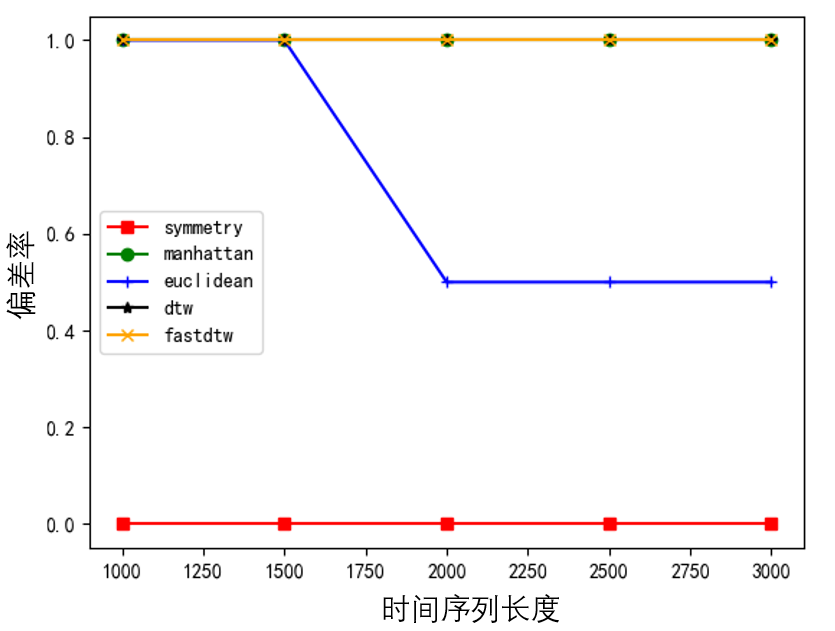
\includegraphics[width=0.43\linewidth]{stock_1.png}}
  \subcaptionbox{金融数据集\label{fig:stock_2}}
  {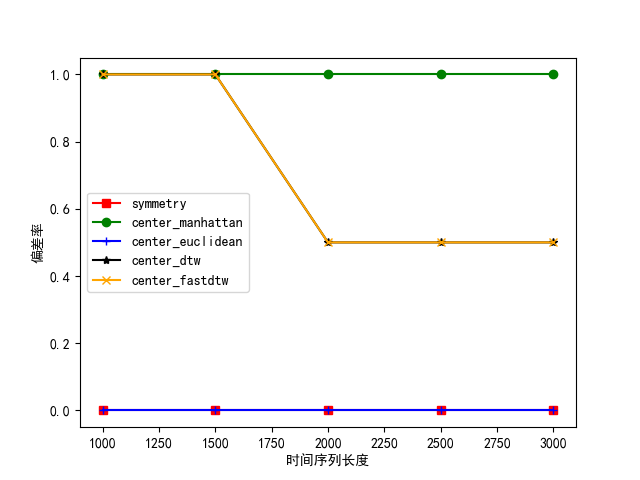
\includegraphics[width=0.43\linewidth]{stock_2.png}}
  \caption{多源时间序列分段对称模式挖掘偏差率结果}
  \label{fig:segement_symmetry}
\end{figure}

\begin{figure}
  \centering
  \subcaptionbox{合成数据集\label{fig:sin_time_1}}
  {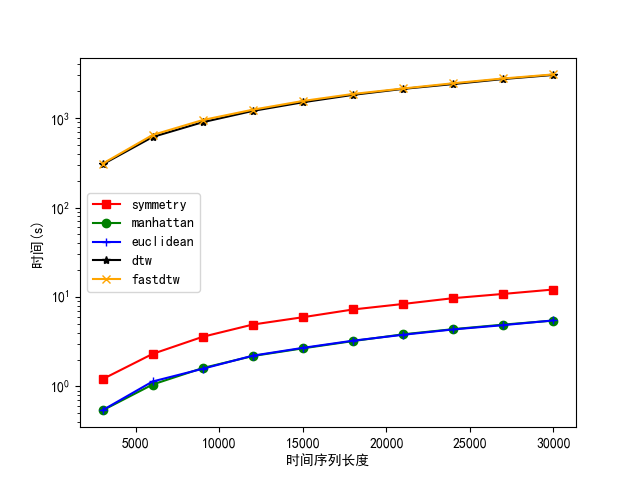
\includegraphics[width=0.43\linewidth]{sin_time_1.png}}
  \subcaptionbox{合成数据集\label{fig:sin_time_2}}
  {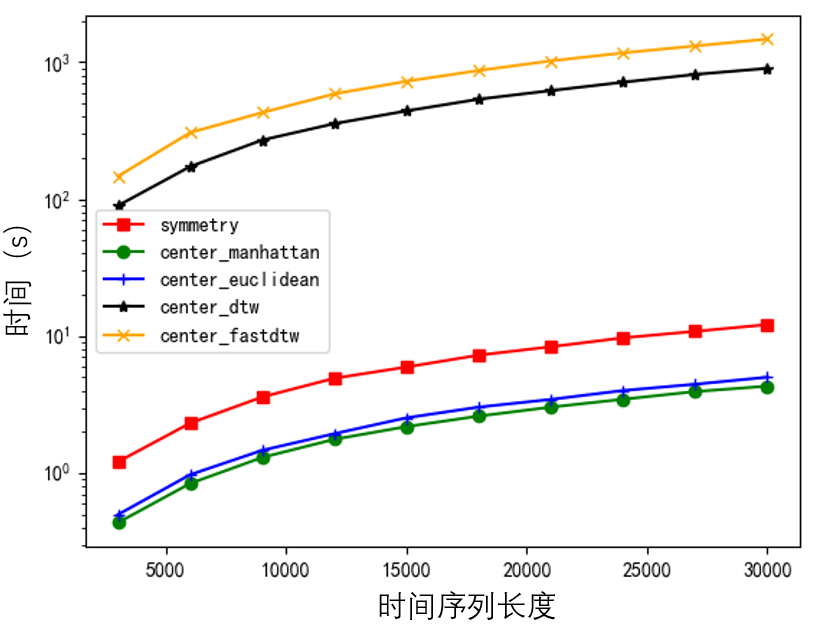
\includegraphics[width=0.43\linewidth]{sin_time_2.png}}
  \subcaptionbox{GPS轨迹数据集\label{fig:truck_time_1}}
  {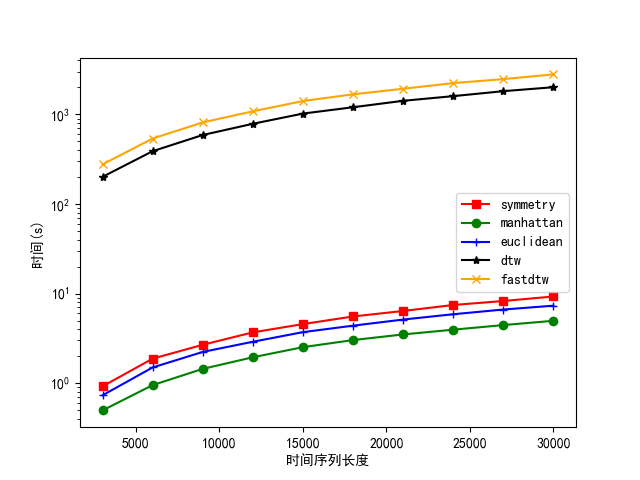
\includegraphics[width=0.43\linewidth]{truck_time_1.png}}
  \subcaptionbox{GPS轨迹数据集\label{fig:truck_time_2}}
  {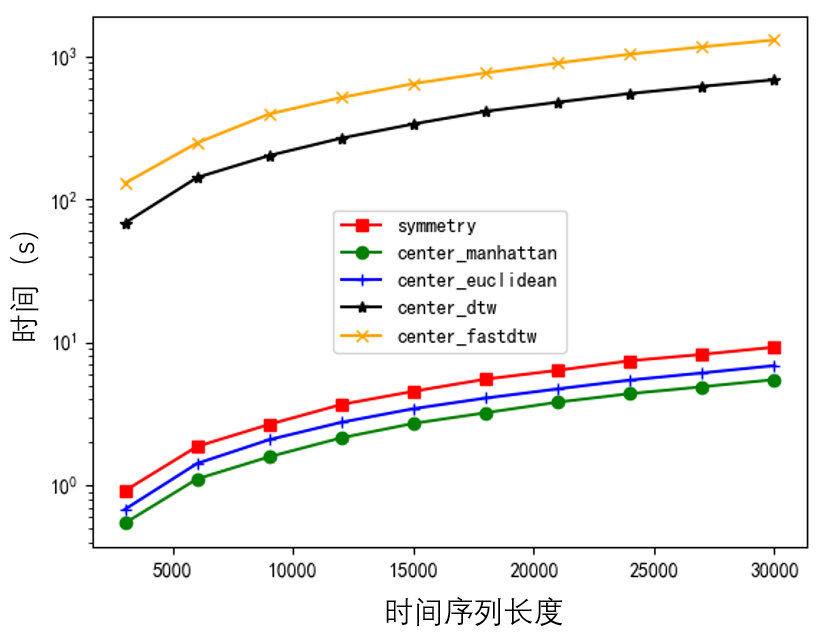
\includegraphics[width=0.43\linewidth]{truck_time_2.png}}
  \subcaptionbox{工况数据集\label{fig:excavator_time_1}}
  {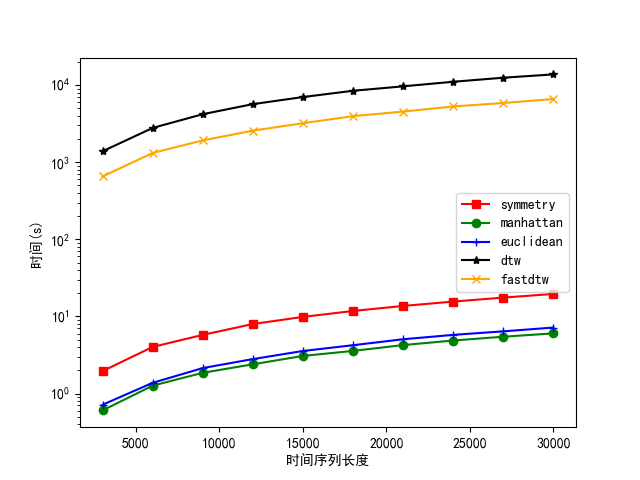
\includegraphics[width=0.43\linewidth]{excavator_time_1.png}}
  \subcaptionbox{工况数据集\label{fig:excavator_time_2}}
  {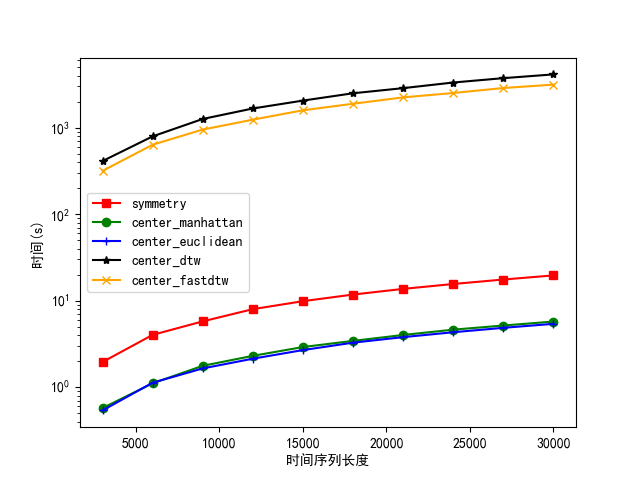
\includegraphics[width=0.43\linewidth]{excavator_time_2.png}}
  \subcaptionbox{金融数据集\label{fig:stock_time_1}}
  {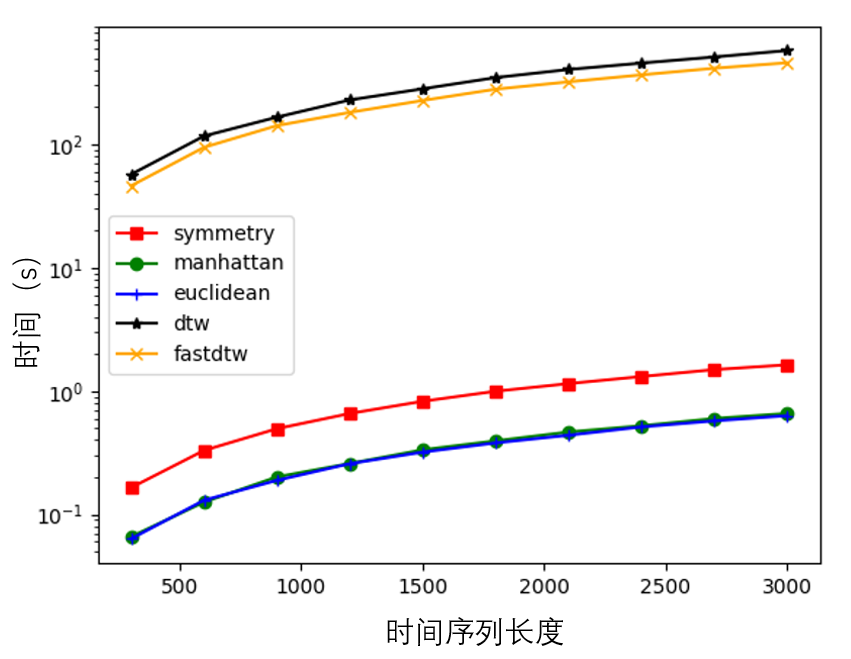
\includegraphics[width=0.43\linewidth]{stock_time_1.png}}
  \subcaptionbox{金融数据集\label{fig:stock_time_2}}
  {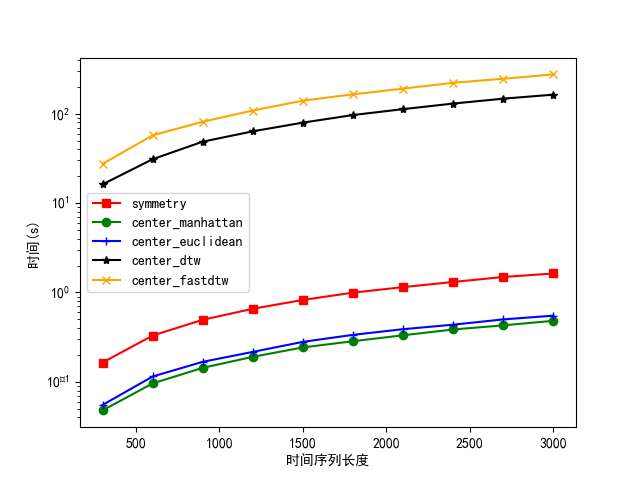
\includegraphics[width=0.43\linewidth]{stock_time_2.png}}
  \caption{多源时间序列分段对称模式挖掘时间效率对比}
  \label{fig:segement_algorithm_time}
\end{figure}

除了比较不同算法挖掘对称模式的效果,本文还对算法的时间性能进行了实验对比。
图~\ref{fig:segement_algorithm_time}展示了所有算法在不同数据集上
随时间序列长度增加而产生的时间开销变化。从图中可以很明显的看出,
分段对称模式挖掘算法的时间效率非常高,十分接近基于曼哈顿距离
和欧氏距离的挖掘方法,而远高于基于DTW距离的方法。
经过对算法复杂度的推导证明,分段对称模式挖掘算法的渐进时间复杂度
为$O\left(n \times w\right)$,而基于DTW距离的挖掘方法
其时间复杂度为$O\left(n \times w^2\right)$。算法时间性能的实验结果证明
了复杂度推导得到的结论。此外,对比图~\ref{fig:excavator_time_1}
和图~\ref{fig:truck_time_1}可知,时间序列的长度变化并不会影响算法
的相对性能,影响算法性能的因素主要是子模式长度约束的大小。
基于DTW距离的算法在运输车GPS数据集上效率高于基于FastDTW距离的算法,
而在挖掘机工况数据集上效率低于基于FastDTW距离的算法,其原因在于
前者对称子模式的平均点数少,实验设定长度约束参数为300。而后者对称子模式
的平均点数多,实验设定长度约束参数为800。FastDTW对DTW进行了剪枝和
抽象优化,其理论渐进时间复杂度为$O\left(w\right)$但实际却无法达到。
因而,在挖掘的对称子模式较长时,使用分段对称模式挖掘算法在效率上会优于
基于FastDTW距离的算法。

\section{本章小结}
本文通过
% !TeX root = ../thuthesis-example.tex

\chapter{系统实现}
在第3章和第4章中,本文设计了全局对称模式挖掘算法和
分段对称模式挖掘算法两种不同的算法,并根据不同应用场景
的特殊约束将其扩展到了流式数据中。
通过第5章中的实验发现,两种对称模式挖掘算法不仅具有最好的
挖掘效果,而且在时间效率上也远远超过基于动态时间扭曲的算法。
接下来,本章基于Apache IoTDB提供的查询分析扩展功能,
将这两种算法集成到数据质量工具库IoTDB-Quality中,
帮助用户挖掘时间序列中蕴含的对称模式信息,
并方便在此基础上执行更复杂的数据分析工作。

\section{总体介绍}
IoTDB-Quality基于IoTDB用户自定义函数(UDF),
实现了一系列关于数据质量和分析的函数,
包括数据画像、数据质量评估与修复、数据匹配和模式发现等,
有效满足了工业领域对数据挖掘的需求。
当对一个时间序列进行数据分析时,
如果能提前识别其中蕴含的模式,用户就能够对
时间序列未来的发展变化具有一个清晰明确的预期,
从而更好地进行预测和分类的工作。

\begin{figure}
    \centering
    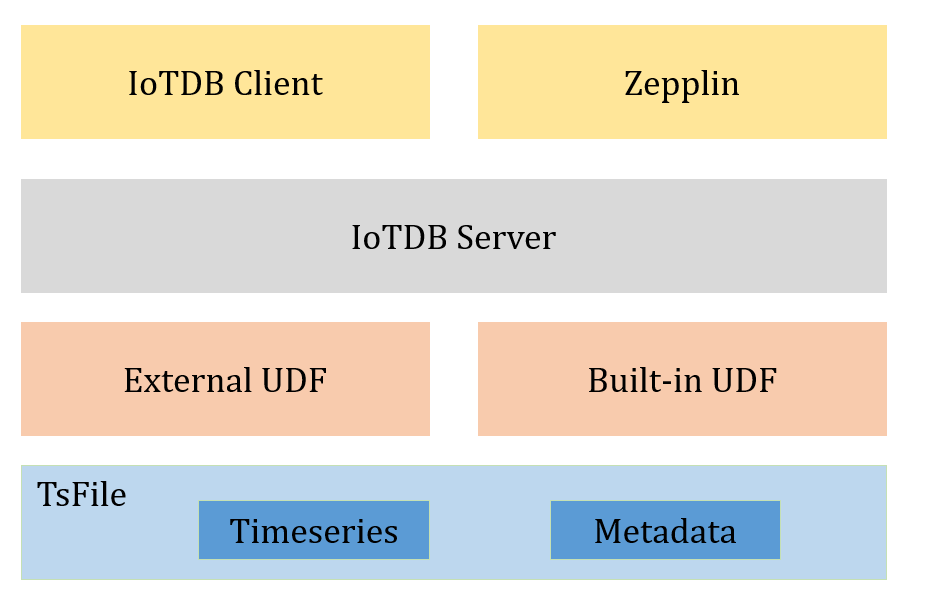
\includegraphics[width=0.66\linewidth]{udf-structure.PNG}
    \caption{基于IoTDB实现的对称模式挖掘算法架构图}
    \label{fig:symmetry_structure}
\end{figure}

% IoTDB为用户提供了一套成熟的函数管理和执行框架,本文的算法实现即基于此框架。
Apache IoTDB为用户提供了一套成熟的函数管理和执行框架,
其底层存储方式也非常方便用户对查询计算功能进行扩展。
如图~\ref{fig:symmetry_structure}所示,IoTDB的数据存储
文件TsFile中不仅存储了时间序列,还存储了与计算查询相关的元数据信息。
根据算法流程对这些数据进行有选择地应用,即可实现原生UDF和
外部UDF两种不同的计算函数。最终这两类UDF都会整合到
IoTDB Server中为用户提供相关的数据分析功能,并将结果
由命令行客户端或Apache UI工具Zepplin进行展示。
根据全局和分段对称模式挖掘算法的计算方式和数据依赖,
本章对全局算法实现了只基于原始时序数据的外部UDF,
而对分段算法则实现了外部UDF和基于元数据的原生UDF两类函数,
尽可能满足不同场景用户的计算需求。


\section{全局对称模式挖掘算法实现}
IoTDB为用户提供了一个用于时间序列数据分析的自定义模板函数接口UDTF
(User Defined Timeseries Generating Function),
该模板支持多条时间序列和多个参数的输入,最终会输出一条时间序列数据
表示函数计算的结果。对于全局对称模式算法而言,根据
图~\ref{fig:global_algorithm_process}所示的计算流程,
只需要输入一条完整的时间序列数据用于挖掘对称模式,具体的
全局对称性度量和对称度阈值确定都可以在函数处理中由算法确定。
在具体实现中,为方便用户使用,本算法提供了阈值(threshold)参数,
可以由领域专家自行指定对称度阈值,若不指定,则采用对称度阈值确定算法进行计算。
\begin{figure}
    \centering
    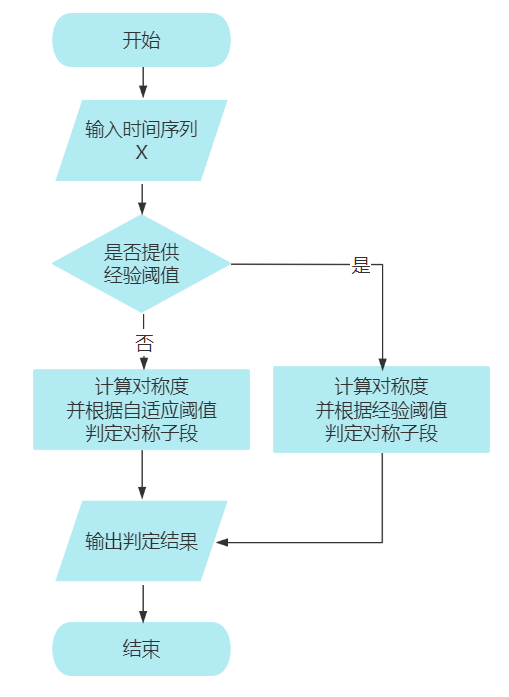
\includegraphics[width=0.55\linewidth]{global_symmetry_algorithm.PNG}
    \caption{全局对称模式挖掘算法流程图}
    \label{fig:global_algorithm_process}
\end{figure}

本算法用到了UDTF中定义的四个接口,具体实现方式如下所示:
\begin{itemize}
\item validate:验证算法的参数是否输入正确,threshold代表时间序列的
      对称度,一定是正数。如果不输入,则代表使用自定义的对称度阈值确定算法。
\item beforeStart:指定滑动窗口的数据访问策略并执行算法的初始化。由于
      全局对称模式挖掘算法是对时间序列整体计算对称性,因此,设定时间序列的
      窗口大小为无穷大以将全部数据加载到算法中。
\item transform:执行全局算法以挖掘对称模式,具体步骤如下所示:
    \begin{enumerate}
        \item 对长度小于2的时间子序列的对称度进行初始化计算。
        \item 按照长度由小到大的顺序推导并计算每一段时间子序列的对称度,并将结果
              保存在预定义的数据结构中。
        \item 根据时间序列的数据特征进行差分计算,得到对称度阈值。
        \item 由计算得到的全局对称度和对称度阈值判定输入时间序列是否属于对称模式。
    \end{enumerate}
\item terminate:将全局时间序列是否具有对称性的判定结果输出到collector中。
\end{itemize}

\section{分段对称模式挖掘算法实现}

分段对称模式挖掘算法的处理过程和全局对称模式挖掘算法有所不同,
分段算法是通过将时间序列划分为不同的子段分别挖掘对称模式的。
结合IoTDB将整条时间序列数据划分为不同的Chunk和Page进行存储,
并在计算时分段计算再合并结果的处理方式,分段算法和IoTDB的存储
计算框架高度契合。正因如此,分段算法既可以像全局算法一样
以外部UDF的方式完成计算,也可以利用每个Page的元数据加速计算。
分段对称模式挖掘算法的外部UDF实现方式非常简单,
直接利用算法~\ref{alg:symmetric_pattern}计算即可。
但分段算法的原生UDF实现方式却需要在计算时考虑元数据,
计算流程较为复杂。

\begin{figure}
    \centering
    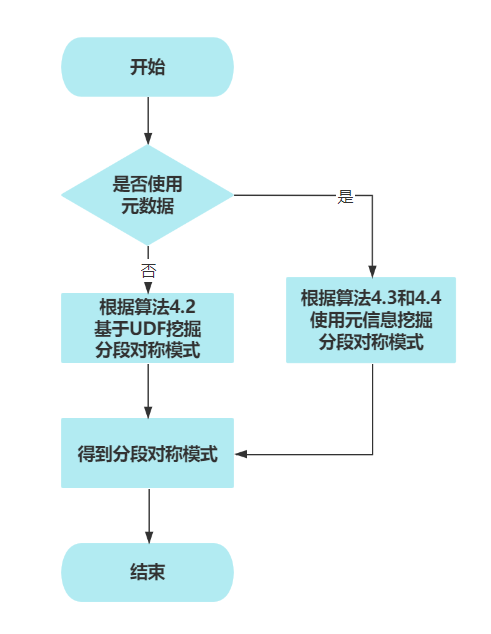
\includegraphics[width=0.55\linewidth]{iotdb_segement_symmetry.PNG}
    \caption{基于IoTDB的分段对称模式挖掘流程}
    \label{fig:iotdb_segement}
  \end{figure}

图~\ref{fig:iotdb_segement}展示了基于IoTDB的分段对称模式
挖掘算法流程。算法在读入时间序列$X$和子序列长度约束$w$之后,
首先需要判断是否存在可以利用的元数据。
元数据的可用性必须满足三个条件,一是
在写入时已完成元数据计算并持久化到TsFile中,
二是写入时从系统配置中读取的子序列长度约束必须和输入的约束$w$
相同,三是查询的范围必须包含完整Page。
经过可用性检验,如果有对应的元数据,则直接合并元数据
就可以得到分段模式的数量。
反之,则还需要重新根据算法4.2加载原始时间序列并挖掘
分段对称模式。最终,算法输出分段对称模式挖掘得到的数量结果。

% 元数据的可用性必须满足三个条件,一是
% 在写入过程中完成计算并持久化到TsFile中,另一个是
% 查询的范围必须包含完整Page。尽管Page中存在元数据但查询时
% 若并未包含Page中所有的时间序列,则仍然需要加载原始数据挖掘对称模式。

% 此外,若要使用


% 因此,在本算法的实现中,对于每一个分段对称模式,算法只输出
% 对称模式的起始时间点和其对称度信息,具体的计算流程如下所示:
% \begin{enumerate}
%     \item 首先,IoTDB通过序列读取器读取时间序列数据,
%     由于需要根据全部子序列的对称度特征进行阈值划分,
%     所以要把所有的数据全部加载到内存中,保存在算法的
%     自定义数据结构中。
%     \item 然后,在transformer函数中定义动态规划
%     状态信息,按照区间由小到大的顺序计算所有长度小于w的
%     子序列的对称度。需要注意的是,由于输出时需要明确分段模式
%     的起始时间,所以需要将RowWindow中每个时间子序列的
%     起始点时间信息保存下来。
%     \item 对transformer函数中保存的数据值进行差分计算,求得
%     相邻点距离的平均值。再采用流式算法计算子序列对称度的方差,
%     根据方差之和最大原则寻找自然断点。利用上述两个阈值候选的最小值
%     求得分段对称模式的真实阈值。
%     \item 根据贪心策略计算出数量最多的对称模式,并将结果循环输出到
%     collector中。
% \end{enumerate}

\section{算法查询展示}

在实现了对称模式挖掘的算法逻辑之后,用户可以使用两种方式
执行算法并对结果进行查询。一种是利用IoTDB-Client命令行,
另一种是在Apache Zepplin上通过前端UI进行查询。
以全局对称模式挖掘数据集和算法为例,
在命令行上,用户登录客户端之后,直接输入调用UDF函数的SQL语句
进行查询,查询结果如图~\ref{fig:iotdb_client_symptn}所示。
直接使用select语句就可以查询全局和分段对称模式的挖掘结果。
使用IoTDB Client命令行进行查询的好处是查询便捷,
直接登陆客户端即可查询,不需要重新部署其他工具。
但是,在命令行查询的结果只能通过表格的方式
进行展示,不方便直观的观察查询结果。仅通过在命令行中观察,
用户无法区分~\ref{fig:gsymptn_input}所示的查询数据是否
具有对称性,因而更无法对查询结果的正确性进行判断。
基于此,在IoTDB-Client上进行查询只适用于开发中的结果验证,
不适合商业化用户使用。因此,需要配置部署一个直观的前端查询方式。
\begin{figure}
    \centering
    \subcaptionbox{GunPoint数据集\label{fig:gsymptn_input}}
    {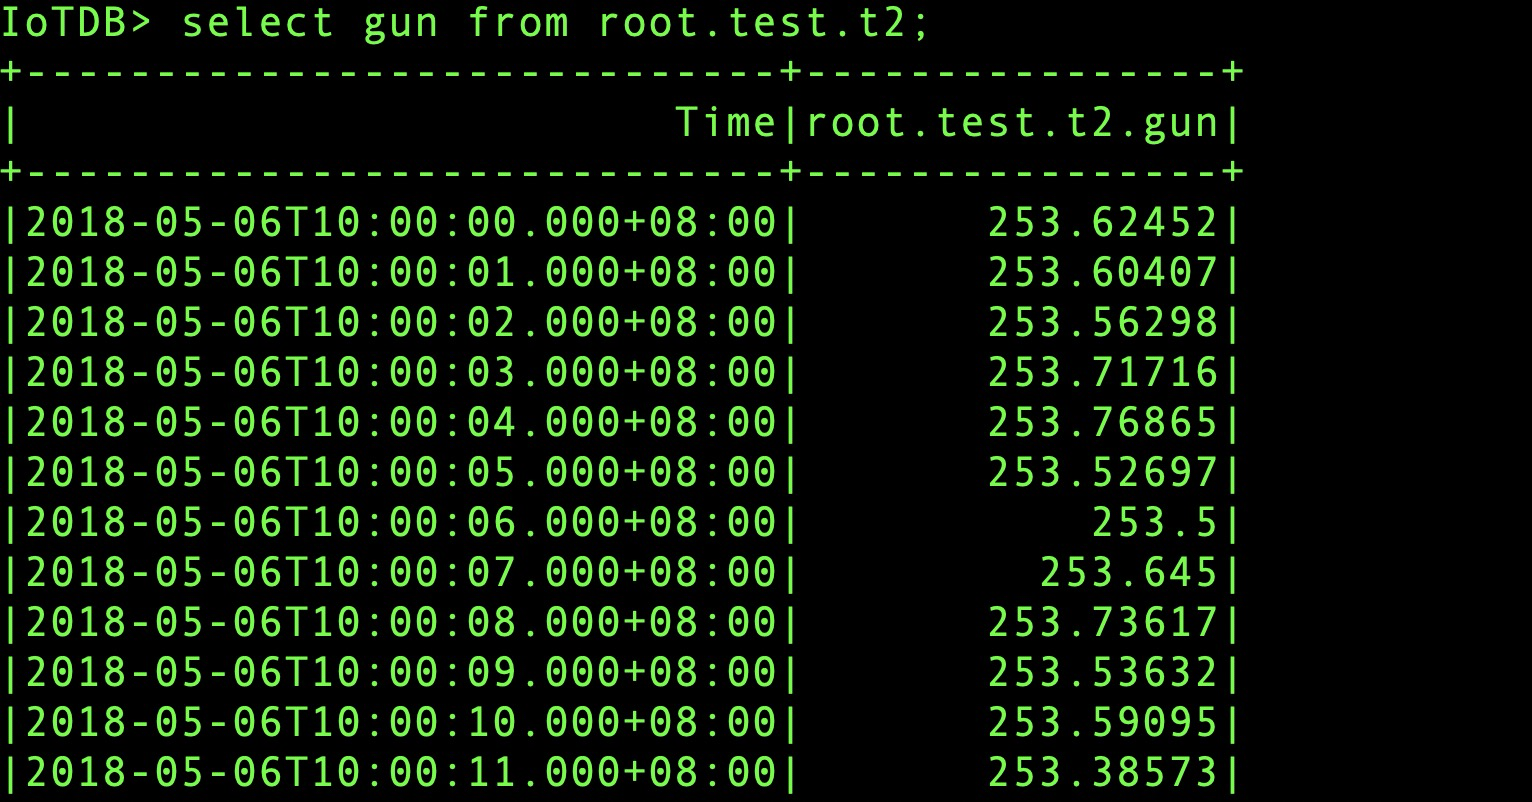
\includegraphics[width=0.86\linewidth]{gun_point_system.png}}
    \subcaptionbox{全局对称模式查询结果\label{fig:gsymptn_output}}
    {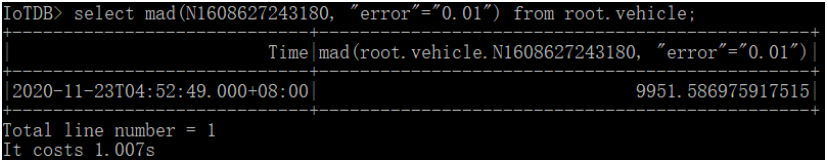
\includegraphics[width=0.86\linewidth]{gsymptn_output.PNG}}
    \caption{在IoTDB-Client运行全局对称模式挖掘算法的结果查询展示}
    \label{fig:iotdb_client_symptn}
\end{figure}

Apache Zepplin是一个是一个基于网页的交互式数据分析系统。
用户可以通过Zeppelin连接IoTDB数据源并使用SQL进行交互式查询操作。
图~\ref{fig:iotdb_zepplin_symptn}中展示了在Zepplin上进行
对称模式挖掘结果计算并查询的方式,图中上半部分是在运输车轨迹GPS经度
数据集中挖掘判定分段对称模式。利用Zepplin自带的散点图和折线图
用户可以方便的观察出运输车轨迹数据集中的时间序列具有16个分段对称模式。
图中下半部分是在运输车轨迹数据集上挖掘分段对称模式,在Zepplin的输入框中直接输入select语句
就可以像IoTDB-Client命令行一样执行查询,
\begin{figure}
    \centering
    \includegraphics[width=0.86\linewidth]{zepplin_truck_data.PNG}
    \caption{运输车轨迹数据集}
    \includegraphics[width=0.86\linewidth]{gsymptn_zepplin.png}
    \caption{在Apache zepplin运行分段对称模式挖掘算法的结果查询展示}
    \label{fig:iotdb_zepplin_symptn}
\end{figure}


\section{本章小结}
本章主要介绍了根据IoTDB提供的用户自定义函数模板接口,
全局对称模式挖掘算法和分段对称模式挖掘算法的实现方式,
并通过在IoTDB Server上进行部署,使用IoTDB Client和
Apache Zepplin两种方式进行函数调用计算和结果查询。
通过基于IoTDB实现这两种算法,弥补了IoTDB Quality挖掘对称模式
的功能缺失,在帮助用户得到蕴含在时间序列中对称特征的同时,
便于发现违反模式规律的异常点并进行检测和修复。
% !TeX root = ../thuthesis-example.tex

\chapter{总结与展望}
\section{论文工作总结}
随着信息技术和工业物联网的发展,数据规模变得越来越大,数据来源
也越来越丰富。在日益多样化的大数据中,时间序列数据是一种应用范围广,
研究价值高的数据类型。针对时间序列的数据分析和模式挖掘,
可以解析构成时间序列的不同成分,提取蕴含在数据内部的高价值知识。
对称模式是一种在时间序列中广泛存在的模式类型,
数据分析从业人员通过挖掘时间序列中的对称模式可以发现
时序数据内部的自相关信息,统计镜像变换的数量指标,得到长期的变化规律。
本文主要研究在多源时间序列数据上进行对称模式挖掘。时间序列对称模式分为两种类型,
全局对称模式和分段对称模式,本文分别针对这两种模式设计了不同的挖掘算法,
并在多源数据集上验证了算法的效果和性能。

对于全局时间序列进行对称模式挖掘,首先需要计算的就是全局时间序列的对称度。
时间序列不同于字符串序列,没有严格的对称中心,由于不同阶段持续时间不同,
前后序列也不一定一一对应进行匹配。然而,本文研究发现无论全局时间序列
如何对应达到最优的匹配效果,第一个点和最后一个点是必然匹配的。
在此基础之上,序列前置点可以倒序和序列后置点进行匹配。
而决定前置点在后置匹配候选点中进行选择的最优化目标不是两点之间的
距离,而是前置点和后置点之间时间子序列的对称性,这形成了一个
具有嵌套结构的子问题。因此,本文基于区间动态规划思想设计了
一个全局时间序列对称性度量算法。在得到时间序列的全局对称度之后,
还需要通过阈值才能将真正的对称模式分类出来。
工业场景中的对称度阈值往往由领域专家设定,但作为一个统一的应用于多源
时间序列对称模式挖掘的算法,阈值需要由算法计算生成。本文研究发现,
相对变化剧烈的时间序列,对称度阈值较大;而相对变化缓和的时间序列,
对称度阈值较小。因此,本文根据时间序列的数据变化特征确定了对称度阈值,
以用于挖掘对称模式。本文在第5章对全局对称模式的挖掘效果进行了评估,
通过在来自UCR的两个具有全局对称性的数据集和两个不具有全局对称性的数据集上
进行实验发现,相比于通过原始和反转时间序列相似性或通过对称中心
两侧子序列相似性度量对称性的方法,本方法不仅能保证挖掘出来的对称模式准确率
很高,在所有挖掘出来的对称模式中的真实对称模式样本比例最高,而且能保证
尽量挖掘出所有的对称模式,在挖掘准确性和完备性之间做了很好的均衡,算法的
综合评价相比其他算法最高。

对于分段时间序列进行对称模式挖掘,首先需要进行时间序列的分段处理,
基于关键点检测的分段方法不仅效率低,而且有可能错误将
对称模式分到不同的子序列中。为保证挖掘出所有的
对称模式,本文设计的分段挖掘算法利用滑动窗口度量了
所有子序列的对称性。为了减少重复计算并尽可能的利用上一个滑动窗口
的状态信息,将全局对称性度量算法进行扩展,引入子序列长度约束参数$w$,
在长度为$n$的时间序列$X$中按照长度由小到大的计算所有不超过$w$的
子序列对称度,然后再根据对称度阈值过滤对称子序列。
对于分段时间序列对称模式而言,除了时序数据变化特征可以用为对称度的约束,
通过对子序列对称度聚类得到的分界点同样可以作为对称度的约束。基于此,本文根据
时序数据特征和对称度分布重新定义了时间子序列的对称度阈值。在过滤得到
所有的对称子序列之后,通过贪心策略选择数量最多且不重叠的对称子序列作为分段对称模式。
本文在第5章中对分段对称模式的挖掘效果和时间效率进行了评估,
通过一个合成数据集和三个来自真实工业与金融业场景的数据集上进行实验,
发现本算法挖掘出来的分段对称模式数量和真实数量偏差最小,远超过
基于一一对应匹配的算法,即使基于动态时间扭曲的算法在挖掘效果上
也并未超过本算法。并且,由于本算法利用滑动窗口对动态规划状态设计进行了
优化,本算法的时间效率和一一对应匹配算法处于同一级别,比基于动态时间扭曲的算法
性能高上了100多倍。

在设计了全局和分段对称模式挖掘算法之后,本文将算法在更多的应用场景上进行了扩展。
首先在研究了在流式数据上挖掘对称模式的方法。本文优化了
全局时间序列对称模式挖掘算法状态推导过程,
在对称度矩阵上创造性地引入了滑动窗口,
在不违反对称度状态连续性和单调性的前提下,采用以空间换时间的
策略将流式对称模式的计算时间复杂度由$O\left(w^2\right)$
提升至了$O\left(w\right)$。此外,本文还在对称模式的
挖掘过程中引入了自适应窗口,通过时间序列的数据特征自动地调节
窗口大小,以保证挖掘对称模式的完整性。在第5章的实验中,
本文在真实工业场景中的数据集上对自适应窗口进行了实验,
发现在变长对称模式存在的场景中,自适应窗口能显著提高对称模式挖掘的完整性。

综上所述,本文设计了在全局和分段时间序列中进行对称模式挖掘的算法,
并通过实验验证,发现本算法不仅具有最好的对称模式挖掘效果,而且在时间效率
上也远高于动态时间扭曲方法,并且通过调整约束可以将本算法推广到流式数据和
变长模式的复杂场景中。同时,本文还将对称模式挖掘算法进行了系统实现,
把这些算法作为自定义函数整合到了IoTDB中,在补全了IoTDB关于对称模式
挖掘的功能缺失之外,还提高了IoTDB对时间序列的分析和预测能力。

\section{未来工作展望}
对称模式挖掘算法挖掘出了时间序列中变换后互为镜像的模式信息,
在轨迹跟踪,行为分析,异常检测等应用场景中均具有重要价值。
基于本文的研究内容,未来还可以开展以下的工作:

一是本文设计的对称性度量算法虽然解决了一一对应的带来的本地
时间偏移和不对齐的问题,但本质上还属于顺序匹配,时间序列前驱点和
后置点之间并不能交叉匹配,如果时间序列带有乱序时间戳的话,则无法识别。
并且,本文的对称性度量算法立足于全局最优匹配,为每个点都计算了最佳匹配点,
虽然利用了时间序列中蕴含的所有信息,但对于个别异常点也进行了匹配。
在异常较多的时间序列中,最好先进行异常检测和修复再利用本算法挖掘对称模式。

二是本文设计的对称度阈值算法对数据集具有一定的局限性。对称度阈值算法
通过时间序列数据特征和对称度分布特征确定了模式对称度的上限,
即对称度小于阈值的即可识别为对称模式。本文设计的
对称性度量算法尽可能的对时间序列进行最优匹配而导致对称度结果较小,
因此,本算法在对称模式较多或者数据变化剧烈的时间序列中具有较好的效果。
而在时间序列变化较平缓且对称模式较少的序列中,可能无法通过算法挖掘出
正确的对称模式。因此,需要根据数据特征再设计确定对称度阈值下限的算法。

最后,本算法挖掘出来的对称模式还可以进行进一步的研究。长度相同的
对称模式不一定具有相同的形状,还可以通过聚类算法挖掘出多类对称模式。
此外,时间序列中蕴含的对称模式数量和类别还可以作为后续分析的特征输入,
可以用来执行分类等任务。






% 其他部分
\backmatter

% 参考文献
\bibliography{ref/refs}  % 参考文献使用 BibTeX 编译
% \printbibliography       % 参考文献使用 BibLaTeX 编译

% 附录
% 本科生需要将附录放到声明之后,个人简历之前
\appendix
% \input{data/appendix-survey}       % 本科生:外文资料的调研阅读报告
% \input{data/appendix-translation}  % 本科生:外文资料的书面翻译
% % !TeX root = ../thuthesis-example.tex

\chapter{补充内容}

附录是与论文内容密切相关、但编入正文又影响整篇论文编排的条理和逻辑性的资料,例如某些重要的数据表格、计算程序、统计表等,是论文主体的补充内容,可根据需要设置。


\section{图表示例}

\subsection{图}

附录中的图片示例(图~\ref{fig:appendix-figure})。

\begin{figure}
  \centering
  \includegraphics[width=0.6\linewidth]{example-image-a.pdf}
  \caption{附录中的图片示例}
  \label{fig:appendix-figure}
\end{figure}


\subsection{表格}

附录中的表格示例(表~\ref{tab:appendix-table})。

\begin{table}
  \centering
  \caption{附录中的表格示例}
  \begin{tabular}{ll}
    \toprule
    文件名          & 描述                         \\
    \midrule
    thuthesis.dtx   & 模板的源文件,包括文档和注释 \\
    thuthesis.cls   & 模板文件                     \\
    thuthesis-*.bst & BibTeX 参考文献表样式文件    \\
    thuthesis-*.bbx & BibLaTeX 参考文献表样式文件  \\
    thuthesis-*.cbx & BibLaTeX 引用样式文件        \\
    \bottomrule
  \end{tabular}
  \label{tab:appendix-table}
\end{table}


\section{数学公式}

附录中的数学公式示例(公式\eqref{eq:appendix-equation})。
\begin{equation}
  \frac{1}{2 \uppi \symup{i}} \int_\gamma f = \sum_{k=1}^m n(\gamma; a_k) \mathscr{R}(f; a_k)
  \label{eq:appendix-equation}
\end{equation}


% 致谢
% !TeX root = ../thuthesis-example.tex

\begin{acknowledgements}
  衷心感谢宋韶旭老师在研究生阶段对我的指导。
  我并不是一个很有学术天赋的人,在一些课题上的研究经常遇到困难。
  每当这个时候,宋老师总能以严谨的学术思维和深厚的学术功底
  为我指明前进的方向。没有宋老师的帮助,我不可能在研究生阶段
  发表一篇论文和申请通过一个专利。在以后的人生道路上,
  宋老师勤奋积极的态度仍然是我指路的明灯。

  感谢实验室的所有同学们,不管是学习还是生活,项目还是科研,
  当我遇到困难的时候,他们总是会尽力地帮助我。感谢东明和浩宇
  学弟在实现系统时对我给予的帮助,使我能较快地优化并完成系统。

  感谢在我成长道路上对我给予帮助的每一个人,感谢父母
  在二十年求学阶段对我的无私关怀和帮助,在我迷茫和
  彷徨的时候,他们总是在我身边。

  本课题承蒙国家自然科学基金资助,特此致谢。
\end{acknowledgements}


% 声明
\statement
% 将签字扫描后的声明文件 scan-statement.pdf 替换原始页面
% \statement[file=scan-statement.pdf]
% 本科生编译生成的声明页默认不加页脚,插入扫描版时再补上;
% 研究生编译生成时有页眉页脚,插入扫描版时不再重复。
% 也可以手动控制是否加页眉页脚
% \statement[page-style=empty]
% \statement[file=scan-statement.pdf, page-style=plain]

% 个人简历、在学期间完成的相关学术成果
% 本科生可以附个人简历,也可以不附个人简历
% !TeX root = ../thuthesis-example.tex

\begin{resume}

  \section*{个人简历}

  1996 年 4 月 1 日出生于河北省保定市。

  2015 年 9 月考入中南大学计算机学院软件工程专业,2019 年 7 月本科毕业并获得工学学士学位。

  2019 年 9 月免试进入清华大学软件学院攻读软件工程硕士至今。


  \section*{在学期间完成的相关学术成果}

  \subsection*{学术论文}

  \begin{achievements}
    \item 李盼盼,宋韶旭,王建民.时间序列对称模式挖掘.软件学报,2022,33(3):968-984.
  \end{achievements}


  \subsection*{专利}

  \begin{achievements}
    \item 宋韶旭, 李盼盼, 王建民. 一种时间序列频繁对称模式挖掘方法及装置: 中国, CN 110990463 B. 2021-01-15.
  \end{achievements}

\end{resume}


% 指导教师/指导小组学术评语
% 本科生不需要
% !TeX root = ../thuthesis-example.tex

\begin{comments}
% \begin{comments}[name = {指导小组学术评语}]
% \begin{comments}[name = {Comments from Thesis Supervisor}]
% \begin{comments}[name = {Comments from Thesis Supervision Committee}]

论文研究时间序列对称模式挖掘,用于轨迹分析、异常识别和序列预测等。选题具有实际应用价值。 
  
论文主要工作包括:  
 
1. 针对单一对称模式,提出了一种对称性度量,以及自适应的对称度阈值确定方法,并设计了最优对称模式求解算法; 
 
2. 针对分段对称模式,提出了基于滑动窗口的时间序列分段处理方法,解决对称子模式重叠问题; 
 
3. 对上述方法进行了实验评估,并在工业物联网时序数据库Apache IoTDB中进行了系统实现。 
 
论文结构清晰,目标明确,通过以上工作表明,李盼盼同学掌握了软件工程的基础理论和对应的专业知识,具备了解决工程问题的方法与手段,具备了独立展开工程技术工作的能力,达到了工程硕士的学术水平,同意组织论文答辩。

\end{comments}


% 答辩委员会决议书
% 本科生不需要
\input{data/resolution}

% 本科生的综合论文训练记录表(扫描版)
% \record{file=scan-record.pdf}

\end{document}
